\documentclass[11pt, a4paper]{scrreprt}

%\usepackage{settings}
\usepackage{amsmath,amstext,amsfonts,amssymb} %Mathe-Formeln

\usepackage{graphicx} %Einbinden von extern erzeugten Grafiken
\graphicspath{{images/}} %Pfad zu den Bildern (einfache Referenzierung)
\usepackage{makeidx}

\usepackage{pdflscape} %Change orientation of specific part
\usepackage{afterpage}
\usepackage{rotating}

\usepackage{xcolor}
\usepackage{fancybox}
\usepackage{ulem} %für Text linien
\usepackage[utf8]{inputenc}
\usepackage[ngerman]{babel}
\usepackage[OT1]{fontenc} % Ligaturen, richtige Umlaute im PDF
%Umschalten der Sprache
\selectlanguage{ngerman}
\usepackage{marvosym}
\DeclareInputText{128}{\EUR}
%Anzeige mathematischer Symbole
\usepackage{amssymb}
%Anzeige von mathematischer Umgebung
\usepackage{amsthm}
\usepackage{stmaryrd}
\usepackage{verbatim}

%f?r integralzeichen Hoch- und Tiefstellung
\usepackage[intlimits]{empheq}
%PDF-Dokumente einbinden
%\usepackage{pdfpages}
%Tabellen einbinden
%\usepackage{booktabs}
\usepackage{tabularx}
%\usepackage{tabular}
\usepackage{hhline}
\usepackage{enumerate}
\usepackage[format = hang, font = {footnotesize, sf}, labelfont = {bf}, margin = 1cm, aboveskip = 5pt, position = bottom]{caption}

%Seitenlayout
\usepackage[left = 2.5cm, right = 2.5cm, top = 1.5cm, bottom = 1.5cm, headheight = 7mm, headsep = 1.2 cm, footskip= 1.5cm, includeheadfoot]{geometry}

%Seitenstil = inhaltliche Gestaltung der Kopf- und Fu?zeile
%\pagestyle{headings}



\usepackage{fancyhdr}
\pagestyle{fancy}
	\fancyhf{}

	\fancyhead[L]{Entwicklung einer Dopplerinstrumentierung zur Detektion von Luftembolin in\\ einen künstlichen Blutkreislauf}
	\fancyhead[R]{
\includegraphics[width=2cm]{images/HS_logo_sw.jpg}}
	\fancyfoot[R]{\thepage}
	\fancyfoot[L]{\nouppercase{\leftmark}}
\fancypagestyle{plain}
{
	\fancyhf{}
		
		\fancyhead[L]{Entwicklung einer Dopplerinstrumentierung zur Detektion von Luftembolin in\\ einen künstlichen Blutkreislauf}
		\fancyhead[R]{
\includegraphics[width=2cm]{images/HS_logo_sw.jpg}}
			\fancyfoot[R]{\thepage}
	\fancyfoot[L]{\nouppercase{\leftmark}}
}
\fancypagestyle{number}
{
	\fancyhf{}
		\fancyfoot[R]{\thepage}		
}

%Zeilenabstand festlegen
\linespread{1.3}


%\newcommand{\HRule}{\rule{\linewidth}{0.5mm}}
%Nullen der Seitenzahl
%\setcounter{page}{0}

%Formelnummerierung anhand der Kapitel
\def\theequation{\thesection.\arabic{equation}}

%Paket zum zitieren
\usepackage{cite}

\usepackage{colortbl} % Um die Zellen innerhalb von \multicolumn farbig darzustellen, muss das Paket colortbl eingebunden werden

%Paket um sprachbezogene Anf?hrungszeichen zu setzen
%\usepackage{csquotes}

%EInbinden des Bibstyles
%\usepackage[backend = biber, style= numeric-comp, sorting = nyt, maxnames = 4, minnames = 1, abbreviate = false]{biblatex}

\newenvironment{myitemize}{\begin{itemize}\itemsep -4pt}{\end{itemize}}

\usepackage{longtable}
%Packet zum Einbinden von Graphiken mit umflie?endem Text
\usepackage{wrapfig}
%Packet zum Benutzen von mehrzeiligen Spalten
\usepackage{multirow}

%Striche raus aus Literaturverzeichnis ????? JM
%\makeatletter
%\def\bstctlcite{\@ifnextchar[{\@bstctlcite}{\@bstctlcite[@auxout]}}
%\def\@bstctlcite[#1]#2{\@bsphack
%  \@for\@citeb:=#2\do{%
%    \edef\@citeb{\expandafter\@firstofone\@citeb}%
%    \if@filesw\immediate\write\csname #1\endcsname{\string\citation{\@citeb}}\fi}%
%  \@esphack}
%\makeatother

%Kapitel etwas weiter nach oben setzen
\renewcommand*\chapterheadstartvskip{\vspace*{-0.2cm}}

\usepackage{indentfirst}

\usepackage{url}

%%
%% Trennungsregeln
%%
\hyphenation{Sil-ben-trenn-ung}

%%
%% Schönere Bullets bei Aufzählungen
%%
\renewcommand{\labelitemi}{$\bullet$}
%\renewcommand{\labelitemii}{$\cdot$}
\renewcommand{\labelitemiii}{$\cdot$}
\renewcommand{\labelitemiv}{$\ast$}
\usepackage{acronym}
%Bilder und Tabellen nebeneinander
\usepackage{caption}
\usepackage{subcaption}

\usepackage{tikz}
\usetikzlibrary{shapes,arrows,automata,matrix,trees}
\usetikzlibrary{decorations.pathreplacing,calc,positioning}
\usetikzlibrary{fit}					% fitting shapes to coordinates
\usepackage{footnote}
\usepackage{tikz-timing}[2009/12/09]
% Use tikz-timing library 'counters' to define a counter character.
% This character draws a 'D{<counter value>}' and increases the counter
% value by one. A reset character which resets the counter value 
% (by default to 1) is also defined.
\usetikztiminglibrary[new={char=Q,reset char=R}]{counters}
%\usepackage[active,tightpage]{preview}
%\PreviewEnvironment{tikzpicture}
\usetikzlibrary{dsp,chains}

\DeclareMathAlphabet{\mathpzc}{OT1}{pzc}{m}{it}
\usepackage{amssymb}
\usepackage{eurosym} %für euronen..
\usepackage{paralist} %lässt sich die Art der Aufzählung ändern
\usetikzlibrary{plotmarks}
\usepackage[active,tightpage]{preview}
\newcommand{\dotprod}{{\scriptscriptstyle \stackrel{\bullet}{{}}}}

% \wraptextureframe{Höhe_in_Zeilen}{Breite}{Text}
% #1 Breite (Anzahl der Zeilen) und variable Höhe
% #2 Text
\newcommand{\wraptextureframe}[2][]{%
  \begin{wrapfigure}{r}{#1}
    \begin{Sbox}
      \begin{minipage}{#1-1em}
        \small\slshape#2%
      \end{minipage}
    \end{Sbox}
    \vskip-2ex%
    \fcolorbox{blue}{gray!0}{\TheSbox}
  \end{wrapfigure}%
}

\newcommand*{\myMarvosymbol}[1]{{\fontfamily{mvs}\fontencoding{U}\fontseries{m}\fontshape{n}\selectfont\char#1}}
\newcommand*{\emailsymbol}{\myMarvosymbol{66}~}
%\usepackage[dvipsnames]{xcolor}
%\usepackage{etoolbox}
%\usepackage{bookmark}
%\usepackage{marvosym}	% Tel. Symbole

\newcommand{\arbeit}{Master Thesis}
\newcommand{\ThesisStart}{15.03.2015}
\newcommand{\ThesisEnd}{15.10.2015}

\newcommand{\fullname}{Andreas Rehn}
\newcommand{\email}{rehn.andreas86@gmail.com}
\newcommand{\mailto}[2]{\href{mailto:#2}{#1}}

\newcommand{\gutachterA}{\href{mailto:brucher@hs-ulm.de}{Prof. Dr.-Ing. Rainer Brucher}}
\newcommand{\gutachterB}{\href{mailto:muenzner@hs-ulm.de}{Prof. Dr.rer.nat., Magister Artium Roland Münzner}}
\newcommand{\street}{König-Wilhelm-Straße 23}
\newcommand{\city}{89073 Ulm}
\newcommand{\university}{Hochschule Ulm}

\newcommand{\titel}{Entwicklung einer Dopplerinstrumentierung zur Detektion von Luftembolin in einen künstlichen Blutkreislauf}
\newcommand{\jahr}{Ulm, den \today}
\newcommand{\fakultaet}{Hochschule Ulm - Fakultät Mechatronik und Medizintechnik}
\newcommand{\institut}{Hochschule Ulm - Institut für Medizintechnik und Mechatronik}
\newcommand{\degree}{Studiengang Systems Engineering und Management - Electrical Engineering}


\usepackage{xspace}
\def\SymbReg{\textsuperscript{\textregistered}\xspace}
\def\SymbC{\textsuperscript{\textcopyright}\xspace}
\def\SymbTM{\textsuperscript{\texttrademark}\xspace}

\setlength{\columnsep}{20pt}
\usepackage{listings}
\usepackage{color}
\renewcommand{\lstlistlistingname}{Quellcodeverzeichnis}
\renewcommand{\lstlistingname}{Quellcode}

\definecolor{mygreen}{rgb}{0,0.6,0}
\definecolor{mygray}{rgb}{0.5,0.5,0.5}
\definecolor{mylilas}{RGB}{170,55,241}

\lstdefinestyle{customc}{
  belowcaptionskip=1\baselineskip,
  breaklines=true,
  frame=L,
  xleftmargin=\parindent,
  language=C,
  showstringspaces=false,
  basicstyle=\footnotesize\ttfamily,
  keywordstyle=\bfseries\color{blue!40!black},
  commentstyle=\itshape\color{green!40!black},
  identifierstyle=\color{black},
  stringstyle=\color{orange},
}

\lstdefinestyle{customverilog}{
belowcaptionskip=1\baselineskip,
breaklines=true,
frame=L,
xleftmargin=\parindent,
language=Verilog,
showstringspaces=false,
basicstyle=\footnotesize\ttfamily,
keywordstyle=\bfseries\color{black},
commentstyle=\itshape\color{mygreen},
identifierstyle=\color{blue},
stringstyle=\color{orange},
}

\lstdefinestyle{Matlab}{
    frame=single,
    breaklines=true,%
    morekeywords={matlab2tikz},
    keywordstyle=\color{blue},%
    morekeywords=[2]{1}, keywordstyle=[2]{\color{black}},
    identifierstyle=\color{black},%
    stringstyle=\color{mylilas},
    commentstyle=\color{mygreen},%
    showstringspaces=false,%without this there will be a symbol in the places where there is a space
    numbers=left,%
    numberstyle={\tiny \color{black}},% size of the numbers
    numbersep=9pt, % this defines how far the numbers are from the text
    emph=[1]{for,end,break},emphstyle=[1]\color{red}, %some words to emphasise
    %emph=[2]{word1,word2}, emphstyle=[2]{style},    
}


\newcommand{\includecode}[4][c]{\lstinputlisting[caption=#3, escapechar=, label=lst:#4, style=custom#1]{#2}}

\newcommand{\includeAttachcode}[3][c]{\lstinputlisting[caption=#3, escapechar=, style=custom#1]{#2}}

\usepackage[hidelinks,unicode]{hyperref}
\usepackage{attachfile} %attach files to pdf :)
\hypersetup{%
	hidelinks,
    %bookmarks=true,         % show bookmarks bar?
	pdfdisplaydoctitle=true,
	bookmarksopen=true,
	pdfpagelayout=OneColumn,% SinglePage / OneColumn 
	% pdfpagetransition={Dissolve},
	% Blinds 	/Dm | Box 	/M | Dissolve | Glitter 	/Di | Split 	/Dm /M | Wipe 	/Di 
	% /Di= direction  in degrees, generally in 90 steps | /Dm horizontal (/H) or vertical (/V) | 
	% /M is motion, in (/I) or out (/O).
    unicode=true,          % non-Latin characters in Acrobat’s bookmarks
    %pdftoolbar=true,        % show Acrobat’s toolbar?
    %pdfmenubar=true,        % show Acrobat’s menu?
    pdffitwindow=true,     % window fit to page when opened
    pdfstartview={FitH},    % fits the FitV/FitH of the page to the window
    pdftitle={\arbeit} { - \titel},    % title
    pdfauthor= {\fullname},     % author
    pdfsubject={\arbeit - \titel},   % subject of the document
    pdfcreator={LaTeX},   % creator of the document
    pdfproducer={PDFLaTeX}, % producer of the document
    pdfkeywords={Signalverarbeitung} {\arbeit} {Hämatokrit} {Cortex-M3} {\titel}, % list of keywords
    pdfnewwindow=true,      % links in new window
    colorlinks=false,       % false: boxed links; true: colored links
    linkcolor=blue,          % color of internal links (change box color with linkbordercolor)
    citecolor=blue,        % color of links to bibliography
    filecolor=blue,      % color of file links
    urlcolor=blue           % color of external links
}
\begin{document}
\pagenumbering{Roman}

\begin{titlepage}
\flushright
\includegraphics[width=5cm]{HS_logo}

\vspace{1 cm}
\begin{center}
\linespread{1}
\LARGE\textbf{\arbeit} \\
\Large{\fakultaet} \\
\large{\degree}
\end{center}

\vspace{2 cm}

\begin{center}
\linespread{1}
\huge{\textbf{\titel}} \\
\vspace{1 cm}
\end{center}

\begin{center}
vom \ThesisStart \ bis \ThesisEnd
\end{center}


\vfill
\begin{tabbing}
1. Gutachter: \= \gutachterA  \kill 
Verfasser: \> \fullname \\
 \> \street \\
 \> \city \\
 \> \email \\
1. Gutachter: \> \gutachterA \\
2. Gutachter: \> \gutachterB \\
\end{tabbing}



\end{titlepage}
\chapter*{Eidesstattliche Erklärung}
\addcontentsline{toc}{chapter}{Eidesstattliche Erklärung}
Hiermit versichere ich, Andreas Rehn, dass ich die vorliegende Arbeit selbstständig und ohne fremde Hilfe verfasst und keine anderen als die angegebenen Quellen oder Hilfsmittel verwendet habe. Alle Ausführungen, die fremden Quellen wörtlich oder sinngemäß entnommen wurden, sind als solche kenntlich gemacht.\\
Ich habe die Bedeutung der eidesstattlichen Versicherung und prüfungsrechtlichen Folgen, sowie die strafrechtlichen Folgen (siehe unten) einer unrichtigen oder unvollständigen eidesstattlichen Versicherung zur Kenntnis genommen.
\\
\\
\section*{Auszug aus dem Strafgesetzbuch (StGB)}
\textbf{§156 StGB} - Falsche Versicherung an Eides Statt\\
Wer von einer zur Abnahme einer Versicherung an Eides Statt zuständigen Behörde eine solche Versicherung falsch abgibt oder unter Berufung auf eine solche Versicherung falsch aussagt, wird mit Freiheitsstrafe bis zu drei Jahren oder mit Geldstrafe bestraft.
\\
\\
\\
\\
\begin{tabbing}
\jahr \= die die Breite der einzelne \= der einzelnen Spalten deklariert \kill %endet mit \kill
\jahr \> \> \fullname \\
\\
\\
\noindent\rule{\textwidth}{1pt}\\
Ort, Datum \> \> Unterschrift \\
\end{tabbing}
\phantomsection
\pdfbookmark{\contentsname}{toc}
\tableofcontents 										%Inhaltsverzeichnis hier anlegen
\phantomsection
\listoffigures 											%Abbildungsverzeichnis
\addcontentsline{toc}{chapter}{Abbildungsverzeichnis}
\phantomsection
\listoftables 											%Tabellenverzeichnis
\addcontentsline{toc}{chapter}{Tabellenverzeichnis}
%\lstlistoflistings
%\addcontentsline{toc}{chapter}{Quellcodeverzeichnis}
\newpage 												%neue Seite
\pagenumbering{arabic}

\chapter{Abkürzungen und Begriffsdefinition}

\section{Abkürzungen} 
\begin{acronym}[mosfetmosfet]\itemsep0pt
\acro{adc}[ADC]{Analog-Digital Converter}
%\acro{alu}[ALU]{Arithmetic logic unit}
\acro{api}[API]{Application programming interface}
\acro{bom}[BOM]{Bill of Materials}
\acro{bzw}[bzw.]{beziehungsweise}
\acro{ca}[ca.]{circa}
%\acro{cad}[CAD]{Computer Aided Design}
\acro{cmsis}[CMSIS]{Cortex Microcontroller Software Interface Standard}
\acro{cw}[CW]{Continuous Wave}
\acro{cpld}[CPLD]{Complex Programmable Logic Device}
\acro{db}[dB]{Dezibel}
\acro{dac}[DAC]{Digital-Analog Converter}
\acro{dc}[DC]{Direct Current}
\acro{dft}[DFT]{Diskrete Fourier Transformation}
\acro{esb}[ESB]{Ersatzschaltbild}
%\acro{eeprom}[EEPROM]{Electrically Erasable Programmable Read Only Memory}
\acro{dh}[d.h.]{das heißt}
\acro{dma}[DMA]{direct memory access}
%\acro{dnf}[DNF]{disjunktive Normalform}
\acro{emi}[EMI]{Electromagnetic interference}
\acro{fft}[FFT]{Fast Fourier Transformation}
\acro{fifo}[FIFO]{First In, First Out}
\acro{fir}[FIR]{finite impulse response}
\acro{fpga}[FPGA]{Field Programmable Gate Array}
%\acro{fps}[FPS]{frames per second}
\acro{fpu}[FPU]{floating-point unit}
\acro{ghz}[GHz]{Giga Herz}
\acro{gui}[GUI]{Graphical User Interface}
\acro{hal}[HAL]{Hardware Abstraction Layer}
\acro{hf}[HF]{Hochfrequenz}
%\acro{hdk}[HDK]{Hardware Development Kit}
\acro{hdl}[HDL]{Hardware Description Language}
%\acro{hkt}[Hkt]{Hämatokrit}
\acro{ic}[IC]{Integrated Circuit}
\acro{ide}[IDE]{integrated development environment}
\acro{iir}[IIR]{infinite impulse response}
%\acro{isbn}[ISBN]{Internationale StandardBuchNummer}
%\acro{ito}[ITO]{Indium-Tin-Oxide}
\acro{khz}[kHz]{Kilohertz}
%\acro{knf}[KNF]{konjunktive Normalform}
\acro{ldo}[LDO]{Low-dropout regulator}
\acro{lna}[LNA]{Low Noise Amplifier}
\acro{lut}[LUT]{Look-up Table}
\acro{ma}[mA]{Milliampere}
\acro{mcu}[MCU]{Microcontroller Unit}
\acro{mhz}[MHz]{Megahertz}
%\acro{mcv}[MCV]{mittleres corpusculäres Volumen der Erythrozyten}
\acro{mosfet}[MOSFET]{metal oxide semiconductor field-effect transistor}
\acro{msps}[MSps]{Megasamples per second}
\acro{nf}[NF]{Niederfrequenz}
\acro{oop}[OOP]{Objektorientierte Programmierung}
\acro{pc}[PC]{Personal Computer}
\acro{pcb}[PCB]{Printed Circuit Board}
%\acro{pla}[PLA]{Programmable Logic Array}
\acro{pp}[pp]{peak-peak}
\acro{prf}[PRF]{Pulse Repetition Frequency}
\acro{pw}[PW]{Pulsed Wave}
%\acro{qfn}[QFN]{Quad-Flat-No-leads (Package)}
\acro{ram}[RAM]{Random-Access Memory}
\acro{rd}[R\&D]{research and development}
\acro{rf}[RF]{Radio Frequenz}
\acro{resp}[resp.]{respektive}
\acro{roi}[ROI]{Region of Interest}
%\acro{rtc}[RTC]{Real Time Clock}
%\acro{saw}[SAW]{Surface Acoustic Wave}
\acro{smd}[SMD]{Surface-mounted device}
\acro{smt}[SMT]{Surface-mount technology}
\acro{sps}[Sps]{samples per second}
\acro{ssp}[SSP]{Streaming Serial Port}
\acro{sfdr}[SFDR]{Spurious-Free Dynamic Range}

\acro{snr}[SNR]{Signal-to-Noise-Ratio}
\acro{spi}[SPI]{Serial Peripheral Interface}
\acro{spp}[SPP]{Streaming Parallel Port}
%\acro{tqfp}[TQFP]{Thin Quad Flat Package}
\acro{ua}[u. a.]{unter anderen}
\acro{uat}[UAT]{User-Acceptance-Test}
\acro{usb}[USB]{Universal Serial Bus}
\acro{vhdl}[VHDL]{Very High Speed Integrated Circuit Hardware Description Language}
\acro{zb}[z.B.]{zum Beispiel}


\end{acronym}

%\begin{table}[!h]
%\caption{Abkürzungsverzeichnis}
%\label{Abkuerzungen}
%\begin{tabularx}{16 cm}{|l|X|}
%\hline
%\textbf{Abkürzung} & \textbf{Beschreibung}\\ \hline 
%a.h & ab hier \\\hline
%ADC & Analog-Digital Converter \\\hline
%\end{tabularx}

%\end{table}


\newpage
\section{Begriffsdefinitionen}\label{sec:begriffe}

\begin{longtable}{|p{5.5cm}|p{9.5cm}|}
KILLED & LINE!!!! \kill
\caption{Begriffsdefinitionen\label{Begriffe}}\\
\hline

\endfirsthead
\caption[]{(Fortsetzung Begriffsdefinitionen)}\\
\hline
\textbf{Begriff} & \textbf{Definition}\\ \hline \endhead
\textbf{Begriff} & \textbf{Definition} \\\hline

%\acf{alu} & Arithmetisch-logische Einheit welche ein elektronisches Rechenwerk in einen Prozessor abbildet. \\ \hline
\acf{api} & engl. Programmierschnittstelle, welche die wichtigsten Funktionen und Eigenschaften eines programmierten Moduls zu Verfügung stellt \\ \hline
\acf{db} & Das Dezibel ist eine nach Alexander Graham Bell benannte Hilfsmaßeinheit zur Kennzeichnung von Pegeln und Maßen (Logarithmische Größe). Diese Größen finden ihre Anwendung \ac{ua} in der Elektrotechnik sowie in der Akustik. \\ \hline
\ac{bom} & engl. Stückliste \\ \hline
%\ac{cad} & rechnerunterstütztes Designen \\ \hline
\acf{cw} Dopplerverfahren  & kontinuierliches Dopplerverfahren \\ \hline
\acf{fir} & Filter mit endlicher Impulsantwort oder Transversalfilter welcher ein diskreter, meist digitaler Filter darstellt\\ \hline
\ac{hal} & engl. Hardwareabstraktionsschicht \\ \hline
\ac{hf} & Frequenzen oberhalb hörbarer Schallwellen \\ \hline
\ac{ide} & engl. integrierte Entwicklungsumgebung \\ \hline
Interface & engl. Schnittstelle zwischen Funktionen oder Geräten \\ \hline
%\ac{ito} & Molekülverbindung aus Indium-Zinn-Oxid \\ \hline
\acf{ldo} & engl. linear Regler mit geringen Verlusten welcher auch mit geringfügig höheren Eingangsspannungen betrieben werden kann.\\ \hline
\ac{lna} & engl. rauscharmer Verstärker, welcher sich durch besondere Rauscharmut auszeichnet \\ \hline
\ac{pcb} & engl. Leiterplatte \\ \hline
\acf{pw} Dopplerverfahren & Gepulstes Dopplerverfahren \\ \hline
Ringing-Effekt	& Einschwingverhalten, welches durch die Steilheit der Flanken unstetiger Signale negativ beeinflusst wird. Dieser Effekt beruht auf dem Gibbssches Phänomen.  \\ \hline
\acf{roi} & engl. Bereich von Interesse \\ \hline
Schallimpedanz & Verhältnis von Schalldruck zu Schallschnelle \\ \hline
%\acf{sfdr} & Störungsfreier dynamischer Bereich - Abstand der größten Störung zur Grundschwingung in einem Spektrum anzugeben.\\ \hline
\acf{snr} & engl. Signal-Rausch-Verhältnis, beschreibt das Verhältnis zwischen Nutzsignal und des Rauschens in der Einheit \ac{db}\\ \hline
\acf{smd} & oberflächenmontiertes Bauelement auf Basis der \acf{smt} \\ \hline
%\acf{saw} & Akustische Oberflächenwelle \\ \hline
Transducer & engl. Schallkopf \\ \hline
\acf{uat} & Ist ein Test, welcher durch den Auftragnehmer durchgeführt wird, um den user die funktionale Sicherheit der Anwendung / des Produktes zu gewährleisten. \\ \hline
\end{longtable}

\chapter{Einleitung und Aufgabenstellung}


\section{Einleitung}
Der Blutkreislauf ist eine der wichtigsten Regeleinrichtungen des menschlichen Organismus. Dieser Kreislauf transportiert Blut, welches sich aus festen - Erythrozyten, Leukozyten und Thrombozyten - und flüssigen - Plasma - Bestandteilen zusammensetzt. Dabei passt sich der Kreislauf an die aktuelle Belastungsart an, indem er die Durchflussgeschwindigkeit des Blutes reguliert. Jedoch ist die Durchflussgeschwindigkeit durch die Herzfrequenz und den Arterienquerschnitten begrenzt.
%Arterien können durch die erhöhte bzw. ungesunde Zufuhr von Nahrungsmitteln sowie Genussmitteln stark belastet werden, da sich Ablagerungen (Gefäßverengung) bilden können oder die Dehnbarkeit der Arterien und somit der maximale Querschnitt reduziert werden kann. 
Dabei kann der Blutfluss durch Ereignisse, sogenannte Embolien, welche in den Gefäßen auftreten gehemmt oder gar zum erliegen gebracht werden. Die Folge ist ein minderperfundiertes betroffenes Gewebe mit anschließenden Absterben von Zellen. Dabei gibt es drei Emboliearten, welche primär in der ambulanten und stationären Behandlung vorherrschen und ein Zellsterben mit sich bringen.
\begin{description}
\item[Luft- / Gasembolie] welche durch Injektion von Gas oder bei schnellen auftauchen aus großen Tiefen\footnote{Taucher- bzw. Dekompressionskrankheit} entstehen können. Injektionen treten meist bei Operationen am offenen Herzen und bei Operationen an Arterien auf.
\item[Tromboembolie] umgangssprachlich auch \glqq Blutgerinnsel\grqq{} genannt, entsteht durch eine Ansammlung von Blutblättchen an der Gefäßwand, welche durch Arterienverkalkungen begünstigt werden kann. Diese Ansammlung kann sich von der Gefäßwand lösen und anschließend die Arterie verschließen.
\item[Fettembolie] ist eine Ansammlung von Fetttröpfchen bzw. Fettzellen, welche nach offenen Knochenbrüchen in den Blutkreislauf eingeschwemmt werden können.
\end{description}
Da diese Ereignisse vermehrt zufällig auftreten und das Risiko mitunter von dem Patienten abhängig ist, wurde für Lungenembolien der Wells-Score nach dem Wissenschaftler P.S. Wells eingeführt. Dieser Score beschreibt die Dringlichkeit und den zu betreibenden Aufwand für eine Diagnose. Des weiteren ist bekannt, dass bei Operationen vermehrt Ereignisse auftreten können, welche jedoch durch die relaxierte Muskulatur des Patienten nur bedingt wahrgenommen werden kann. Ein Monitoring zentraler Arterien während der Patient narkotisiert ist, könnte Embolien aufdecken und somit ein schnelle Entscheidungsfindung bei Schlaganfällen oder Lungenembolien begünstigen.\\
Die zeitnahe Erkennung von Ereignissen ist somit von zentraler Bedeutung für jeden behandelnden Arzt, da in der operativen Medizin jeder Zeit -  \glqq Time is Brain\grqq{}, \glqq Time is Muscle\grqq{} und \glqq Golden hour\footnote{Zeit zum verhindern schlimmerer Sachen}\grqq{} - Komplikationen auftreten können. Die Erkennung eines Ereignisses erlaubt es dem Arzt zu entscheiden, ob die Operation weitergeführt werden kann oder abgebrochen werden muss. Dabei hat ein Abbruch der Operation eine Lysetherapie mit einer erhöhten Dosis Heparin gegen die erkannte Embolie zur Folge.\\
Ein Monitoring von Ereignissen sollte an den Hauptarterien durchgeführt werden, da diese einen erhöhten Volumenstrom und somit eine erhöhte Chance auf die Erkennung von Ereignissen bieten. Dabei sind invasive\footnote{latein invadere \textit{einfallen, eindringen}} Methoden nicht zu empfehlen, da diese Gewebeschäden zur Folge haben. Eine Alternative bieten nicht invasive Methoden, da diese den Patienten nicht verletzen und das Gewebe zerstören wodurch eine Beobachtung von Gehirnarterien ermöglicht werden kann.\\
Die vorliegende Arbeit befasst sich aus diesem Grund mit der Umsetzung einer nicht invasiven Methode zur schnellen und eindeutigen Emboliedetektion.

\section{Aufgabenstellung}
\subsection{Aufgabenstellung der Masterarbeit}
Ziel dieser Arbeit ist die Realisierung eines Systems für die eindeutige Detektion von Embolien auf Basis der nichtinvasiven gepulsten Ultraschall-Dopplertechnologie. Eine Visualisierung in Spektrogramm und M-Mode sowie die akustische Wiedergabe der Signale sind dabei unverzichtbar, um möglichst viele Informationen aus der zeitnahen Messung zu generieren und somit eine eindeutige Detektion zu gewährleisten. \autoref{fig:usdschema} visualisiert dabei das grundlegende Vorhaben.\\
Diese Thesis soll \ac{ua} eine Optimierung einer vorhandenen Hardware darstellen, da eine Detektion von Ereignissen durch die Messgenauigkeit des Messsystems bedingt ist. Beim Designen der Elektronik ist darauf zu achten, dass verschiedene Ultraschallsonden verwendet werden können. Des Weiteren soll eine Optimierung der bereits entwickelten Schnittstelle zum \ac{pc} erfolgen, da die aktuelle Datentransferrate für eine eindeutige Detektion von Embolien nicht ideal erscheint. Zudem muss ein Algorithmus implementiert werden, um Embolien eindeutig zu detektieren und dem Nutzer zu visualisieren. Die Visualisierung der Messung soll dabei auf einen \ac{pc} unter Nutzung diverser Betriebssysteme erfolgen indem eine benutzerfreundliche \ac{gui} bereitgestellt wird. Alle weiteren Details werden in \autoref{sec:sysreq} spezifiziert.
\begin{figure}[ht]
	\centering
	\begin{subfigure}[b]{0.49\textwidth}
		\centering
  		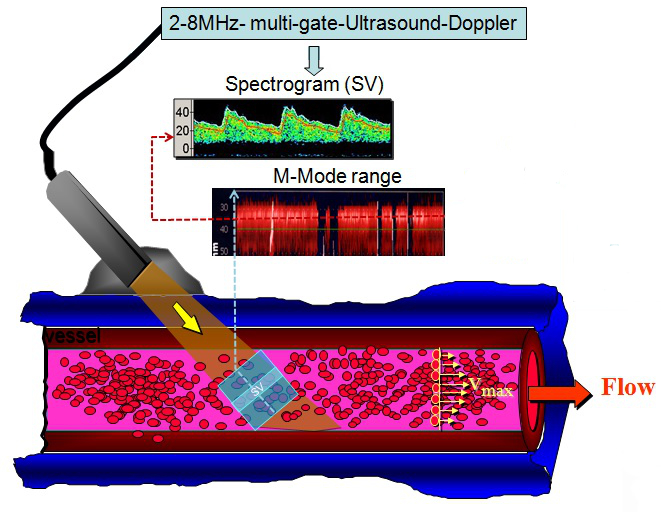
\includegraphics[trim = 0mm 0cm 0cm 0cm, clip=true, width=0.9\textwidth]{pw/USDSchema}  
		\caption{Methodik mit M-Mode und Spektrogramm}
  	\end{subfigure}
  	\hfill
  	\begin{subfigure}[b]{0.49\textwidth}
	  	\centering
  		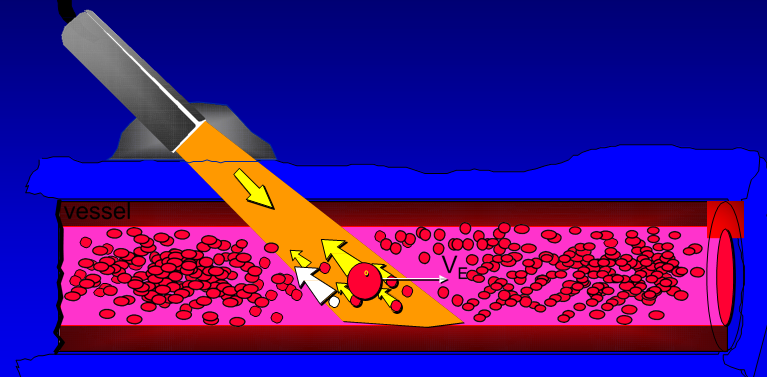
\includegraphics[trim = 0mm 0cm 0cm 0cm, clip=true, width=0.9\textwidth]{emboMeasure}
	  	\caption{Emboliedetektion mittels Ultraschall Doppler}
  	\end{subfigure}
	\caption{Vereinfachte Darstellung des Vorhabens}
  	\label{fig:usdschema}
\end{figure}
%
%
%

\subsection{Vorstellung des vorhandenen Systems}
\subsubsection*{Das digitale Ultraschall-Multigate-Doppler System - Version 2012}\label{cp:usdV1}

Herr Sebastian Stemplewitz entwickelte in seiner Bachelorarbeit an der Hochschule Ulm einen Prototypen für die \ac{pc} gestützte Hämatokritwertmessung. Dieser sollte eine kostengünstige und intravasale Alternative zur aktuellen Hämatokritwertbestimmung werden.\\
Das System ist soweit minimalisiert sowie miniaturisiert(\autoref{fig:system_stemp}), dass eine Weiterentwicklung des Systems die logische Schlussfolge war. Messdaten können erfolgreich mit 8 MHz Sonden aufgenommen und darstellen werden. Dabei dient ein PIC18F4550 \ac{mcu} der Firma Microchip als Schnittstelle zwischen der Messsteuerung und dem \ac{pc} durch die Implementierung eines \ac{usb} Audio-Profils, welches mit der selbst entwickelten Software\footnote{auf Basis von C++ und QT} kommuniziert. Jedoch wurde in der Testphase festgestellt, dass eine Optimierung der Transmitter- und Receiverschaltung notwendig ist um Artefakte zu reduzieren und die Messgenauigkeit zu erhöhen. Aus dem Wunsch, die Kompatibilität mit 2 und 4 MHz Ultraschallsonden zu gewährleisten, entstand die Idee dieses System mit einen ARM-Cortex \ac{mcu} zu betreiben und die Datenverarbeitung und Darstellung über diesen bereitzustellen.\cite{stemp2012}
\newpage
\begin{figure}[h]
\centering
  	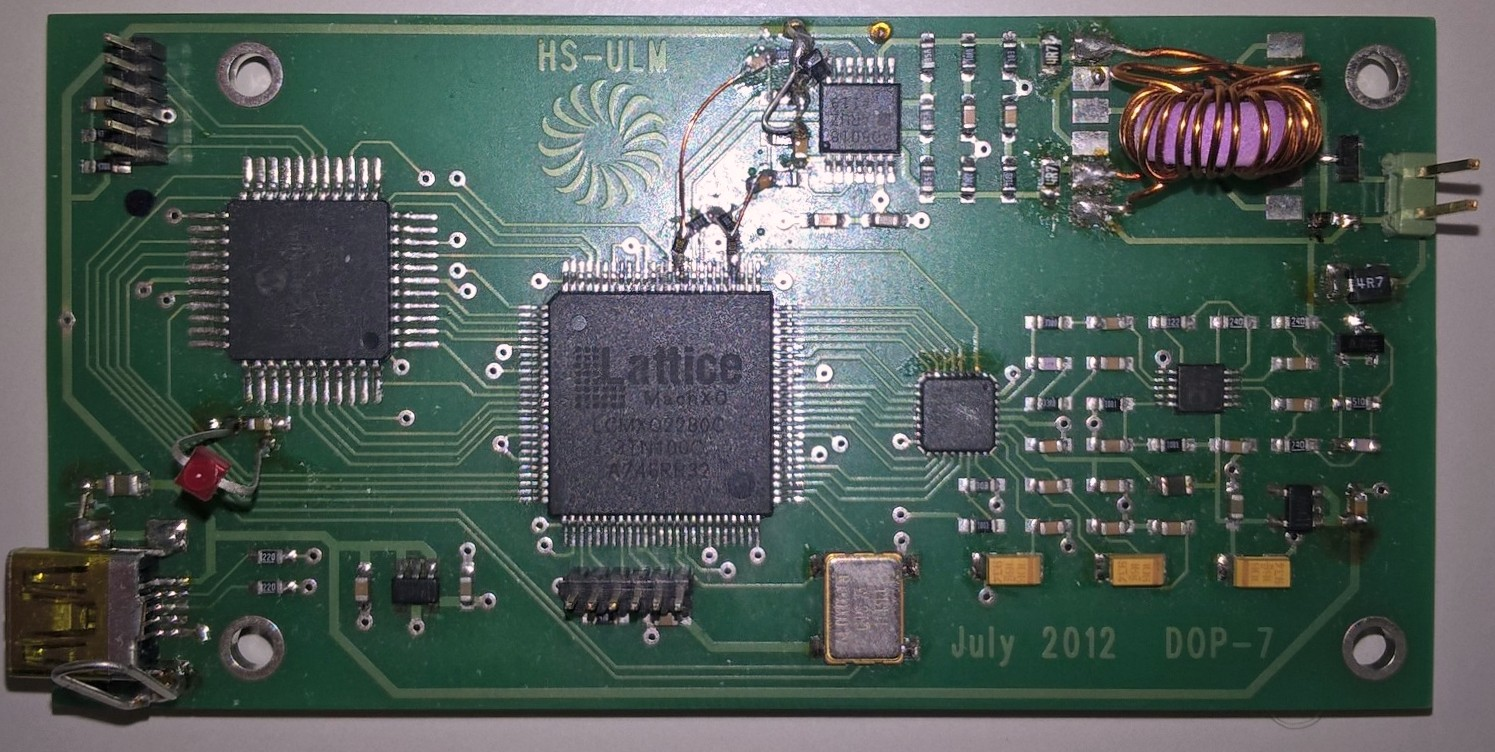
\includegraphics[width=\textwidth]{systemV1}  
	\caption{Systemaufbau Thesis Stemplewitz}
  	\label{fig:system_stemp}
\end{figure}
\begin{table}[h]
\centering
\caption{Bestandteile der Platine}
\label{tab:system_stemp_tab}
\begin{tabular}{c|l}
\textbf{Nr.} & \textbf{Beschreibung} \\
\cline{1-2}
1 & \ac{mcu} und \ac{usb}-Kommunikation\\ 
2 & Signalerzeugung und Dempdulation \ac{cpld}\\ 
3 & Transmitter mit Differenzverstärker und Übertrager\\ 
4 & Receiver mit Vorverstärker und \ac{adc}\\ 
\end{tabular}
\end{table}

\subsubsection*{Das digitale Ultraschall-Multigate-Doppler System - Version 2014}\label{cp:usdV2}
Herr Andreas Rehn, Autor dieser Arbeit, optimierte in seiner Bachelorarbeit an der Hochschule Ulm die Version 2012 (\autoref{cp:usdV1}) für die Hämatokritwertmessung. Dabei wurde das Messsystem modularisiert und ein ARM-Cortex M3 \ac{mcu} für den Datentransfer sowie für die Ansteuerung eines LCD-Displays integriert. Dabei stellte sich heraus, dass das vorhandene \ac{cpld} für die mathematische Vorverarbeitung der Signale keine Reserven bietet. Außerdem konnte eine Steigerung der Flexibilität durch die Umstrukturierung des Zustandsautomaten erreicht werden. Die Datentransferrate zwischen \ac{cpld} und \ac{mcu} wurde auf 15,7 Mbit/s gesteigert, welche durch das \ac{usb} Full-Speed Interface auf 12 Mbit/s (brutto) begrenzt ist. Messungen ergaben weiterhin, dass das 2-Layer Layout und die Schaltung nicht ideal sind, da ein Spannungsoffset von durchschnittlich 11 mV und ein \ac{snr} von 59 \ac{db} nach der Digitalisierung ermittelt wurden. Daher ergab sich der Wunsch, die Datentransferrate durch eine alternative Schnittstelle sowie die Messgenauigkeit des Systems zu erhöhen und die Signalverarbeitung zu optimieren.\cite{rehn2014}

\begin{figure}[h]
\centering
  	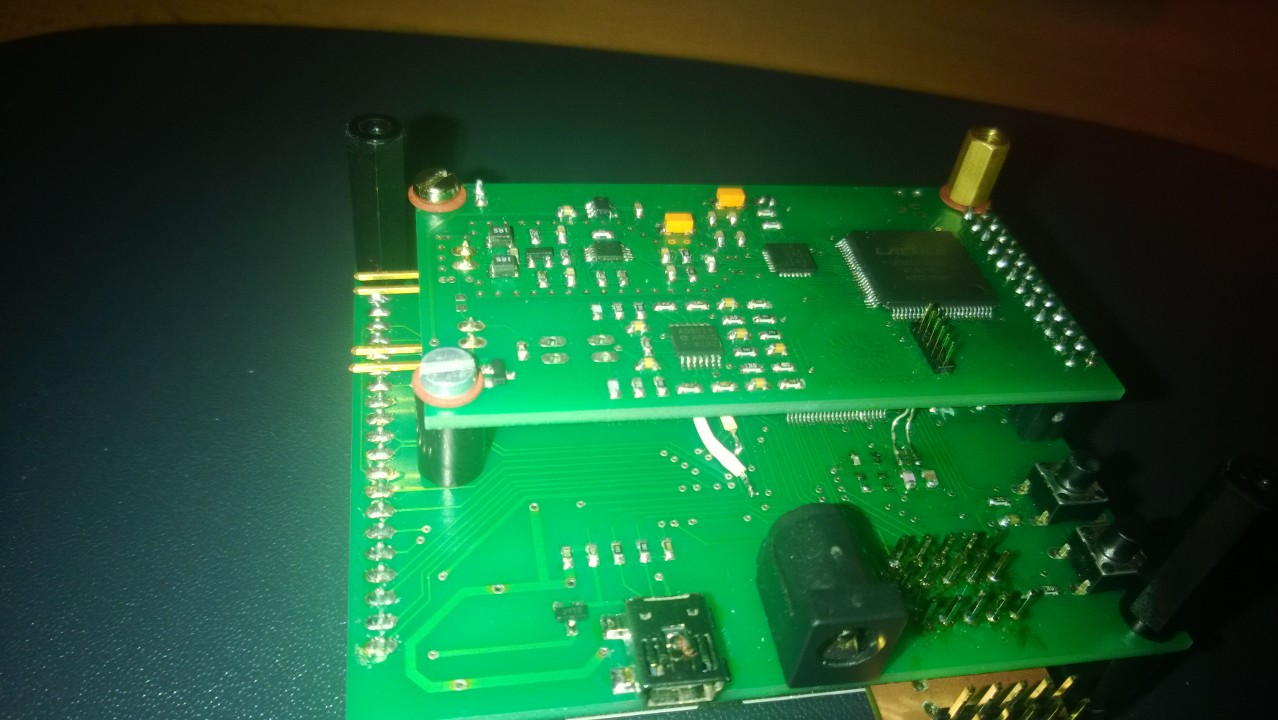
\includegraphics[trim = 10cm 0cm 2cm 5cm, clip=true, width=\textwidth]{systemV2}  
	\caption{Systemaufbau Thesis Rehn}
  	\label{fig:system_stemp}
\end{figure}
\begin{table}[h]
\centering
\caption{Bestandteile der Platine}
\label{tab:system_stemp_tab}
\begin{tabular}{c|l}
\textbf{Nr.} & \textbf{Beschreibung} \\
\cline{1-2}
1 & \ac{cpld} mit Signalerzeugung und Demodulation\\ 
2 & Receiver mit Vorverstärker und \ac{adc}\\
3 & Transmitter mit Differenzverstärker und Übertrager\\
4 & Interface TFT LCD-Display\\
5 & \ac{mcu} mit \ac{usb}-Kommunikation\\
\end{tabular}
\end{table}
%
%
%
\newpage
\subsection{Anforderungen an das Messsystem}\label{sec:anforderungen}
Es werden drei Ebenen von Anforderungen unterschieden: die Benutzeranforderungen, die Systemanforderungen und die Software- und Hardwareanforderungen.\newline
Benutzer und deren Anforderungen werden dabei als höchste Ebene angesehen, da sie die Bedürfnisse des Kunden an das System darstellen. Darunter werden sowohl grundlegende Anforderung, Basisanforderungen sowie Begeisterungsfaktoren beschrieben, welche entschlüsselt, gegliedert und anschließend strukturiert werden müssen.\\
Die grundlegenden Anforderungen, welche Richtlinien und Normen beinhalteten, müssen erfüllt sein. Basisanforderungen beschreiben die Funktionalität des Systems. Nur wenn grundlegende, sowie Basisanforderungen erfüllt sind, kann das System zertifiziert, auf den Markt gebracht und dem Kunden die Möglichkeit gewährt werden, das Produkt zu kaufen. Begeisterungsfaktoren sind Anforderungen, die aus Sicht des Kunden nicht unbedingt erfüllt sein müssen um das Produkt zu kaufen. Jedoch bewegen genau diese Faktoren den Kunden, das Produkt zu kaufen, da es sich durch diese von Konkurrenzprodukten abheben kann. Benutzeranforderungen enthalten derweil keinerlei technische Vorgaben.\newline
Systemanforderungen bilden die mittlere Anforderungsebene, welche die allgemeinen Leistungen des Produktes spezifiziert. Diese Leistungen dienen als Grundlage des Systemdesigns.\newline
Die Software- und Hardwareanforderungen werden aus dem Systemdesign abgeleitet und detaillierter beschrieben.\newline % wodurch die Software- und Hardwaredesign abgeleitet werden.\newline
Bindende und optionale Anforderungen können anhand der Kundenformulierung unterschieden werden. Dabei werden bindende Anforderungen durch "'soll"' oder "'darf nicht"' hervorgehoben. Normativ bindende Anforderungen werden durch "'muss"' Formulierungen dargestellt. Eine optionale Anforderung wird dabei durch "'sollte"' und eine Zusatzfunktion mit "'kann"' formuliert.\newline
Die in dieser Arbeit durchgeführte Optimierung wurde durch die folgenden Anforderungen detailliert definiert.
\subsection*{Benutzeranforderungen}
\begin{itemize}\itemsep0pt
\item Das bestehende USD-System soll aus einer Messplatine bestehen.
\item Das System soll mit Ultraschallsonden im Frequenzbereich von 2, 4 und 8 \ac{mhz} arbeiten.
\item Für eine \ac{prf} sollen mindestens 40 Werte (20 Real-, 20 Imaginärteil) zu Verfügung gestellt werden, um weitere Analysen zu ermöglichen.
\item Das System soll über eine \ac{pc} Software betrieben werden können.
\item Die \ac{pc} Software soll auf den Betriebssystemen Linux und Windows funktionieren.
\end{itemize}
\subsection*{Systemanforderungen}\label{sec:sysreq}
\begin{itemize}\itemsep0pt
\item Das System soll über eine externe Spannungsversorgung betrieben werden, welche den Normen entspricht.
\item Das System soll als Steuereinheit einen ARM-Cortex M4 besitzen.
%\item Das System soll einen funktionsfähigen Audioausgang besitzen.
%\item Das System sollte einen Composite-Out Ausgang besitzen.
\item Das System soll einen USB-micro Anschluss besitzen.
%\item Die Messplatine soll einen Triggerausgang für die Zertifizierung von Ultraschallsonden bereitstellen.
%\item Das System soll einen separaten Ausgang sowie Eingang für Messungen bereitstellen, welche leicht miteinander verbunden werden können.
\end{itemize}
\subsection*{Software- und Hardwareanforderungen}
\begin{itemize}\itemsep0pt
	\item \textbf{Energieversorgung}
	\begin{itemize}\itemsep0pt
		\item Das System soll die Hardware des Energieversorgers vor Fehlfunktionen des Systems schützen.%vor was? Je nach detaillierter Anforderung kann das ziemlich aufwändig werden. Wie würdest Du die Hardware z.B. vor einem Flugzeugabsturz schützen?
		%\item Das System sollte eine maximale Leistungsaufnahme von 2.5W bei 5V DC besitzen.
		\item Das System soll mit einer maximalen Eingangspannung von 20V betrieben werden können.
		\item Das System soll aus der angelegten Spannung die für das System benötigten Spannungen erzeugen.
	\end{itemize}
\end{itemize}
\begin{itemize}\itemsep0pt
	\item \textbf{Messelektronik}
	\begin{itemize}\itemsep0pt
		\item Die Messelektronik soll eine Spannungsversorgung von 3,3 V besitzen.
%		\item Die Messelektronik soll separat aus einer Platine bestehen.
%		\item Ein Trigger Signal sollte vorhanden sein, um das Zertifizierungsverfahren der Sonden und des Systems zu ermöglichen.
		\item Die Messelektronik sollte den \ac{emi} Richtlinien entsprechen.
		\item Die Messelektronik sollte einen Schutz vor zu großen Signalamplituden besitzen.
		\item Die Messelektronik soll eine \ac{prf} von 2 kHz bis zu 12 kHz und eine Abtastrate von 64 MHz besitzen.
		\item Die Platine soll eine steckbare Verbindung für die Sonde aufweisen.
		\item Die Messelektronik sollte über eine Codierung die Frequenz der angeschlossenen Sonde erkennen können.
	\end{itemize}
\end{itemize}
\begin{itemize}\itemsep0pt
	\item \textbf{Auswerteelektronik}
	\begin{itemize}\itemsep0pt
		\item Die Auswerteelektronik soll eine Schnittstelle zu einen \ac{pc} besitzen, welche mindestens eine Datentransferrate von 100 Mbit/s unterstützt.
		\item Eine Visualisierung der aktuell angeschlossenen Sonde mit deren Frequenz sollte vorhanden sein, um den Nutzer eine schnelle Identifizierung der Sonde zu ermöglichen.
	\end{itemize}
\end{itemize}
\begin{itemize}\itemsep0pt
	\item \textbf{\ac{gui}}
	\begin{itemize}\itemsep0pt
		\item Das \ac{gui} soll ein Menu bereitstellen, um die Parameter der Messung einzustellen.
		\item Das \ac{gui} soll ein linearen, für die Messwerte und ein \ac{fft}-Graphen, für das Zeit-Schallsignal bereitstellen.
	\end{itemize}
\end{itemize}
%
%
%
\section{Beschreibung der Methodik}
Die Ausgangssituation wurde analysiert und mit dem aktuellen Stand der Forschung verglichen, indem die zur Verfügung stehenden Unterlagen studiert und mit aktueller Fachliteratur abgeglichen wurden. Durch die Recherchen des aktuellen Stands der Technik zeigte sich entsprechendes Optimierungspotenzial im Vergleich zu den vorhandenen Messsystemen. Insbesondere zeigte sich, dass eine deutliche Verbesserung der Nutzbarkeit erreicht werden kann, wenn eine Datentransfersteigerung des Systems erreicht werden kann. Desweiteren ergab sich Optimierungspotential in der Messgenauigkeit. Durch die Anpassung der Hard- und Software und der Anpassung des Layouts unter Beirücksichtung gängiger \ac{emi} Aspekte, wurden im Rahmen der hier beschriebenen Studienarbeit grundlegend Verbesserungen im Hinblick auf die Genauigkeit der Messung und des Nutzungskomforts des Messystems erreicht. %done

\chapter{Grundlagen}
\section{Ultraschall}
\subsection{Definition}
Schallwellen sind mechanische Wellen. Dabei unterscheidet man Infraschall\footnote{Frequenzen $< 20$ Hz}, Ultraschall\footnote{Frequenzen $>20.000$ Hz \ac{bzw} 20 kHz} und Schallwellen, welche das menschliche Gehör wahrnehmen kann\footnote{Frequenzen von 20 bis 20.000 Hz}.
\begin{figure}[h]
		\centering
  		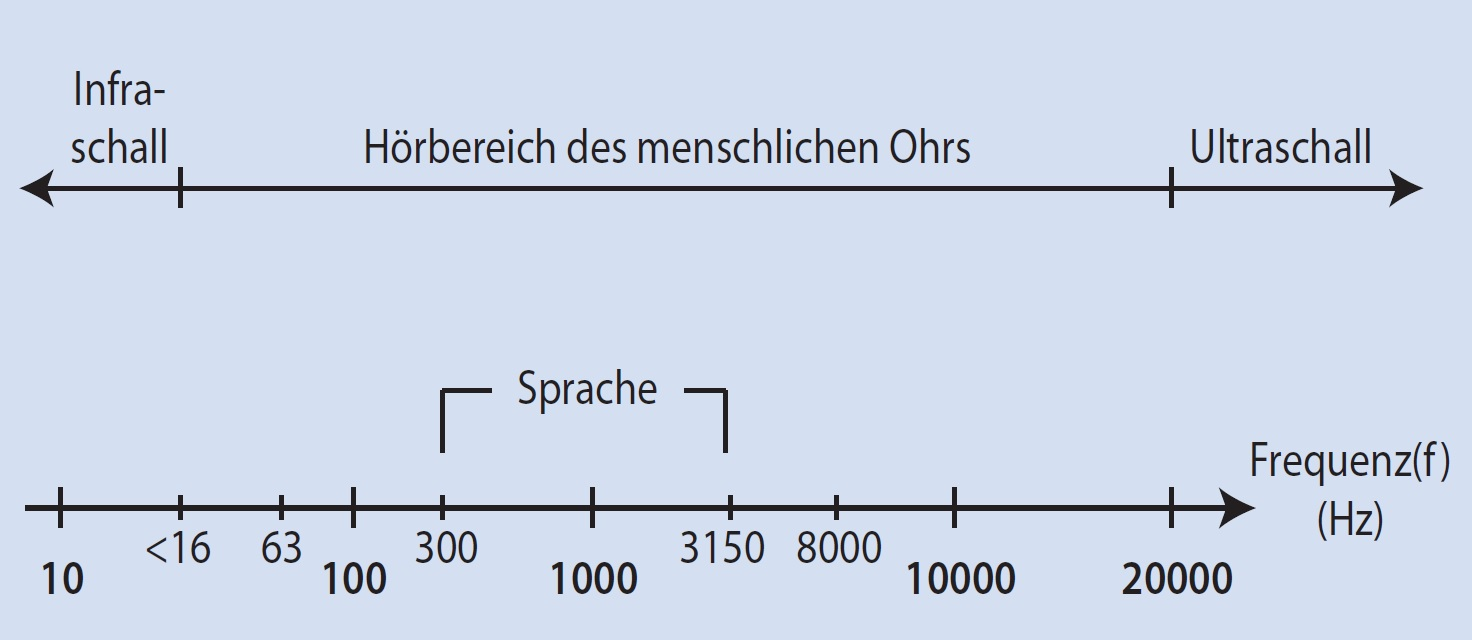
\includegraphics[trim = 0cm 0.5cm 0cm 1.5cm, clip=true, width=\textwidth]{Schall}  
  		\caption{Frequenzbereiche Schall}
  		\label{fig:Schall}
  	\end{figure}
Die höchsten, technisch realisierbaren Schallfrequenzen liegen bei \ac{ca} 1 \ac{ghz}. Für die medizinische Diagnostik sind dabei Frequenzen im Bereich von 2 bis 10 \ac{mhz} interessant. Unterhalb von 2 \ac{mhz} ist die Auflösung zu gering und oberhalb von \ac{ca} 10 \ac{mhz} ist die Absorption im Gewebe zu stark.\newline
In menschlichem Gewebe beträgt die Schallgeschwindigkeit $c$ etwa 1500 $m/s$. Bei Frequenzen im Bereich von 2 bis 10 \ac{mhz} ist deshalb die Wellenlänge $\lambda$ im Bereich von $<$ 10 mm. Somit kann man erreichen, dass sich Ultraschall im Gewebe wie ein optischer Strahl ausbreitet. Er kann fokussiert, reflektiert, gestreut und absorbiert werden. Durch diese Effekte kann somit eine Abbildung von Organen erzielt werden, welche die Basis der Sonographie oder Ultraschalldiagnostik bildet.%
\cite{suter2006}\cite{suter2009}\cite{suter2010}
%
\subsection{Erzeugung und Empfang}
Im Jahr 1880 wurde der \textit{Piezoelektrische Effekt} von Pierre Curie entdeckt. Der Effekt bezieht sich auf Materialien, welche einen permanenten elektrischen Dipolmoment\footnote{Materialien, bei denen die Schwerpunkte der positiven und negativen Ladungen nicht zusammenfallen} aufweisen. Diese erzeugen eine Spannung, wenn eine Kraft (\ac{resp} ein Druck) angelegt wird.\\
Mit diesem Effekt ist es möglich Kräfte, jedoch aber auch Torsion oder wie in dieser Arbeit Ultraschall zu messen. 
\begin{figure}[hb]
	\centering
	\begin{subfigure}[b]{0.49\textwidth}
		\centering
  		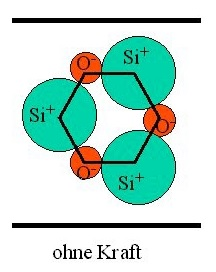
\includegraphics[trim = 0mm 10mm 0mm 0mm, clip, scale=0.5]{Piezo_without}  
  		\caption{ohne Kraft}
  		\label{fig:piezo_without}
  	\end{subfigure}
  	\hfill
  	\begin{subfigure}[b]{0.49\textwidth}
	  	\centering
  		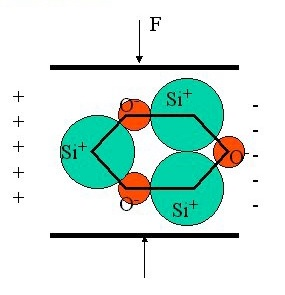
\includegraphics[trim = 0mm 10mm 0mm 0mm, clip, scale=0.5]{Piezo_with}  
  		\caption{Ein Druck erzeugt eine Kraft}
  		\label{fig:piezo_with}
  	\end{subfigure}
  	\caption{Piezoelektrischer Effekt}
  	\label{fig:piezo}
\end{figure}
Dieser Effekt kann aber auch zur Erzeugung von Kraft in Form von mechanischen Wellen genutzt werden. Dies bezeichnet man als den \textit{Indirekten piezoelektrischen Effekt}. Durch Anlegen einer Wechselspannung an einen elastischen Körper wird dieser mit der Frequenz der Wechselspannung verformt und erzeugt in Abhängigkeit der Körpereigenschaften, der Amplitude der angelegten Wechselspannung und deren Frequenz Schallwellen.
%
\cite{suter2006}\cite{suter2009}\cite{suter2010}
%
\subsection{Ausbreitung}\label{sec:ausbreitung}
Eine Schallwelle entspricht einer zeitlichen und räumlichen periodischen Auslenkung von Druck und Dichte des Mediums. Dabei interessieren vor allem die Änderungen des Drucks (nicht der Mittelwert). Somit sind Schallwellen an Materie gebunden und können sich im Vakuum nicht ausbreiten. In Luft, Flüssigkeiten sowie biologischen Gewebe breiten sich Schallwellen dabei in Form von Longitudinalwellen\footnote{von Zonen mit Über- und Unterdruck (Verdichtungs- und Verdünnungszonen)} aus. \\
Dabei hängt die Schallgeschwindigkeit $c$ in Festkörpern von der Dichte \(\rho\), der Poissonzahl \(\mu\) und dem Elastizitätsmodul \(E\) ab. Es ist dabei die Schallgeschwindigkeit $c$ im Festkörper:
\begin{equation}
c_{longitudinal}=\sqrt{\dfrac{E(1-\mu)}{\rho(1-\mu-2\mu^2)}}\label{eq:c_long}
\end{equation}
\begin{equation}
c_{transversal}=\sqrt{\dfrac{E}{2\rho(1+\mu)}}\label{eq:c_trans}
\end{equation}
Mit der \autoref{eq:c_long} werden für die Medizin wichtigen Schallgeschwindigkeiten für die aufgeführten Materialien bestimmt (siehe \autoref{tab:Schallgeschwindigkeiten}).
Der Schalldruck und die Schallimpedanz darf dabei nicht vernachlässigt werden, da die Ausbreitung von Druck und Dichte des Mediums abhängig ist.\\
Für die Schallimpedanz $Z$ findet man:
\begin{equation}
Z=\dfrac{\Delta\rho_0}{\upsilon_0}=\sqrt{K\cdot\rho_0}
\label{eq:z over rho}
\end{equation}
\begin{equation}
Z=c\cdot\rho
\label{eq:z over c}
\end{equation}
Aus den Gleichungen \ref{eq:z over rho} und \ref{eq:z over c} ist erkennbar, dass die Schallimpedanz $Z$ eine Materialkonstante ist.\newline
Die Intensität einer Schallschwelle\footnote{Energietransport pro Fläche und Zeiteinheit} ist
\begin{equation}
j=\dfrac{\text{Kraft $\cdot$ Weg}}{\text{Fläche $\cdot$ Zeit}}=\rho\cdot c
\label{eq:j}
\end{equation}
Mit der kinetischen Energiedichte \(\rho v^2\) kann die Schallintensität auch ausgedrückt werden durch
\begin{equation}
j=\rho c v^2
\end{equation}
In Bezug auf die Zeit ist sie damit
\begin{equation}
j=\rho_0 c A_0^2\omega^2 sin^2(\omega t)
\end{equation}
wobei die Amplitude \(A_0\) die Auslenkung \(A_0 sin(\omega t)\) darstellt.
%
\cite{suter2006}\cite{suter2009}\cite{suter2010}
%
\subsection{Reflexion und Brechung}\label{sec:schall_reflection}
Wie alle Wellen werden auch Schallwellen an Grenzflächen teilweise reflektiert. Diese Grenzflächen befinden sich zwischen Gebieten mit unterschiedlicher Schallimpedanz.
Bei senkrechtem Einfall im linearen Bereich gilt für die transmittierte Intensität $I_t$ mit der emittierten Intensität $I_e$
\begin{equation}
\frac{I_t}{I_e}=4\dfrac{Z_1Z_2}{(Z_1+Z_2)^2}
\end{equation}
und für die Intensität der reflektierten Welle $I_r$
\begin{equation}
\frac{I_r}{I_e}=\dfrac{(Z_1-Z_2)^2}{(Z_1+Z_2)^2}
\label{eq:i of reflection}
\end{equation}
Da in der Sonographie hauptsächlich mit den reflektierten Wellen gearbeitet wird, beziehen sich die nächsten Aussagen auf die \autoref{eq:i of reflection}. Unter Betrachtung der \autoref{tab:Schallgeschwindigkeiten}  und der \autoref{eq:z over c} erschließt sich, dass die Schallimpedanzen der biologischen Materialien sehr gering sind. Somit kann \autoref{eq:i of reflection} weiter vereinfacht und der Reflektionsfaktor $R$ bestimmt werden.
\begin{equation}
R\approx \dfrac{\left(\Delta Z\right)^2}{4Z^2}
\end{equation}
Hingegen ist der Reflektionsfaktor zwischen Luft und dem biologischen Gewebe extrem groß und reduziert die Intensität dementsprechend stark. Diesem Effekt muss durch ein spezielles Kontaktgel entgegengewirkt werden.
%
\cite{suter2006}\cite{suter2009}\cite{suter2010}
%
\subsection{Absorption und Streuung}
Wie in \autoref{sec:schall_reflection} dargestellt nimmt die Gesamtintensität der Ultraschallwelle bei jeder Grenzfläche ab. Zudem wird das Medium durch die einstrahlende Welle in Schwingung versetzt und strahlt somit selbst eine Welle aus. \\
Findet diese Schwingung in Phase mit der einfallenden Welle statt\footnote{homogenes Medium}, beeinflusst die Interferenz zwischen den Wellen lediglich die Phasengeschwindigkeit der Ultraschallwelle.\\
Eine Überlagerung der Wellen hingegen\footnote{in inhomogenen Medium} führt zu einer Schallabstrahlung in alle Richtungen und somit zu einer Streuung, was eine Dämpfung zu Folge hat.\newline
Da das biologische Gewebe jedoch eher einem homogenen Medium entspricht, ist die Abnahme für eine ebene Welle proportional zur Intensität und nimmt somit exponentiell ab
\begin{equation}
I(x)=I_0e^{-\mu x}
\end{equation}
Dabei besteht der Dämpfungs- oder Schwächungskoeffizient $\mu$ aus einem Absorptions- und einem Streuanteil \(\mu = \mu_{Abs}+\mu_{Streu}\). Im Gewebe beträgt die Dämpfung \ac{ca} $1\dfrac{dB}{cm\ \ac{mhz}}$ 
Die Effizienz der Streuung hängt von der Frequenz / Wellenlänge $\lambda$, der Größe der streuenden Inhomogenitäten und dem Unterschied der Schallimpedanz ab. \\
Streuung und Absorption bestimmen zusammen die Eindringtiefe der Schallwellen.
Somit ist die Dämpfung abhängig von dem \textbf{Koeffizienten \(\mu\)}, dem \textbf{Weg \(x\)} und der \textbf{Sendefrequenz \(f\)}.
%
\cite{suter2006}\cite{suter2009}\cite{suter2010}
%
\subsection{Dopplereffekt}\label{sec:dopplereffekt}
Der Effekt tritt bei allen mechanischen Wellen auf, die sich durch den Raum bewegen. Dabei erregt die Welle stationäre und sich bewegende Teilchen gleichermaßen, wodurch eine weitere Welle durch das erregte Teilchen ausgesendet wird. Bei stationären Teilchen wird die Trägerfrequenz $f_0$ reflektiert. Die bewegenden Teilchen jedoch führen je nach Bewegungsrichtung zur Welle kinetische Energie zu der Reflektion der Welle hinzu oder ab\footnote{Teilchen können beschleunigt oder abgebremst werden}. Bewegt sich ein Teilchen entgegen der Longitudinalwellenrichtung so wird die reflektierte Wellenlänge $\lambda$ größer. Umgekehrt wird $\lambda$ kleiner, wenn sich ein Teilchen mit der Longitudinalwellenrichtung bewegt.\newline
Die Differenz $\Delta f$ zwischen emittierter und empfangener Trägerfrequenz nennt man Dopplerschiebefrequenz. Die Differenz ist abhängig von der Trägerfrequenz $f$ und dem Geschwindigkeitsvektor $\overrightarrow{v}$ des bewegten Teilchens. Somit ist der Winkel $\theta$ zwischen Ausbreitungsrichtung der Welle und des Richtungsvektors des Teilchens nicht vernachlässigbar.\\
Die Dopplerschiebefrequenz berechnet sich nach folgender Gleichung
\begin{equation}
\Delta f=\dfrac{2fv\ cos(\theta)}{c}
\end{equation}
Anwendung findet dieser Effekt nicht nur in der diagnostischen Medizin zur Bestimmung von Blutströmungsgeschwindigkeiten. Der Effekt dient seit Jahren in der Industrie und in Haushalten zur Überwachung des Durchflussvolumens und der Erkennung von Fremdkörpern in Flüssigkeiten. Die Dopplerschiebefrequenzen liegen dabei in der diagnostischen Medizin im hörbaren Bereich von einigen kHz.

\section{\acl{pw} Dopplerverfahren}\label{sec:pw}
Beim gepulsten Dopperverfahren werden Bursts\footnote{kurz-gepulste Energiepakete} durch den Transduktor in Kombination mit einen Piezoelement erzeugt. Diese werden in periodischen Abständen (\acf{prf}) in das zu messende Material transmittiert. Dabei werden durch Teilchen oder Dichteänderungen Reflexionen verursacht (\autoref{sec:schall_reflection}), welche mit demselben Piezoelement erfasst und anhand der Laufzeit (\autoref{sec:ausbreitung}) bestimmten Materialtiefen zugeordnet werden kann.\\
Statische Reflexionen verursachen dabei stärkere Signale als die dynamischen Dopplersignale und müssen nachträglich aus der Messung gefiltert werden. Dies geschieht durch die sogenannte Demodulation.\\
\autoref{fig:pw_timing} visualisiert den Ereignisablauf für zwei überlagerte Messtiefen in Abhängigkeit der Peripherieansteuerung. Dabei wird die \ac{prf} durch den Impuls \textit{Retransmit} realisiert, welches die Erzeugung des Burstsignals zur Folge hat. Anschließend werden durch die Zeitdifferenzen, die zu messenden Tiefenbereiche digitalisiert sowie demoduliert. Dabei wird für jeden Tiefenbereich bzw. für jede \ac{roi} eine bestimmte Anzahl von Messwerten generiert und zusammengefasst.\\
\definecolor{fgblue}{rgb}{0,0,0.6}%
\definecolor{fgred}{rgb}{0.6,0,0}%
\begin{figure}[h!]
\centering
\begin{tikztimingtable}
[timing/d/background/.style={fill=white},
timing/c/.cd]
Clock 			& 185{0.2C} \\
\acs{prf} 			& D{}35D{}D{} \\
BURST 			& [fgblue] L 10{0.1H 0.1L} 33L 5{0.1H 0.1L} \\
ADC				& [fgblue] 5L 30H 2L \\
\ac{roi} 1 	& [fgred] 5L 10{2D{}} 12L \\
\ac{roi} 2 	& [fgred] 15L 10{2D{}} 2L \\
Retransmit		& L G 35L G L \\
\extracode
	\draw (0 ,0) circle (0.5 pt); % Origin
	\begin{pgfonlayer}{background}
		\vertlines [help lines]{1,3,5,15,25,35,36}
	\end{pgfonlayer}
%	\tablegrid
\end{tikztimingtable}
\caption{Ereignis-Zeitdiagramm}
\label{fig:pw_timing}
\end{figure}
\hfill
\begin{table}[h!t]
\centering
\caption{Schallgeschwindigkeiten in unterschiedlichen Materialien und Geweben}
\label{tab:Schallgeschwindigkeiten}
\begin{tabular}{l|r}
\textbf{Material} & \textbf{c $\left[\frac{m}{s}\right]$} \\
\cline{1-2}
Luft 				  & $340$	 \\ 
Fett 				  & $1400$	 \\ 
Wasser $(37^\circ C)$ & $1540$	 \\ 
Leber 				  & $1549$ 	 \\ 
Niere 				  & $1561$ 	 \\ 
Muskel 				  & $1568$ 	 \\ 
Blut 				  & $1570$ 	 \\ 
Knochen 			  & $3600$ 	 \\ 
\end{tabular}
\end{table}
\begin{table}[h!t]
\centering
\caption{Eindringtiefen als Funktion der Frequenz in menschlichen Geweben}
\label{tab:Eindringtiefen}
\begin{tabular}{l|l|l}
\textbf{Frequenz f in $\ac{mhz}$} & \textbf{Eindringtiefe in $cm$} & \textbf{Anwendung} \\
\cline{1-3}
1 	& 50	& 	 \\ 
3.5 & 15	& Fötus, Leber, Herz, Niere	 \\ 
5 	& 10	& Gehirn \\ 
7.5 & 7 	& Prostata \\ 
10 	& 5 	& Pankreas \\ 
20 	& 1.2 	& Auge, Haut \\ 
40 	& 0.6 	& Intravaskulär \\ 
\end{tabular}
\end{table} %done

\chapter{Stand der Technik}
\section{Ultrasound Applikation}
ddas hier ist 

\section{\acs{emi} und mixed-Signal \acs{pcb}}

Die symmetrische Signalübertragung (Störfestigkeit) Seite 140f.
ab 500 \ac{mhz} trägt das filterlayout bei (S190) -> Filterlayout vernachlässigbar
Seite 235 - Kleinrechner boards pi filter..

Gegentakt / Gleichtaktstörungen
Galvanische Kopplung und Gegenmaßnahmen
Kapazitive Kopplung und Gegenmaßnahmen
Induktive Kopplung und Gegenmaßnahmen
Filter
Filterschaltungen (Seite 127f.)
Prinzip, Tiefpass, 
\begin{comment}
\section{Transducer}
Um die elektrische Energie in mechanische Energie und umgekehrt zu wandeln wird ein Transducer benötigt, welches gleichzeitig das Kernstück der Ultraschallsonographie darstellt.\\
Dieser besteht wie in \autoref{Abkuerzungen} gezeigt aus einen oder mehreren Piezoelementen mit der dazugehörigen matching-Schicht für die verbesserte Fokussierung. Da die longitudinal Wellen auf beiden Seiten eines Piezoelementes entstehen, müssen die Wellen auf der Rückseite der Sonde absorbiert werden um Reflektionen zu vermeiden. Dies geschieht durch einen einen akustischen Absorber und einen \textbf{backing block}. Zudem muss die Sonde vor \ac{emi} Störungen geschützt werden, da das Piezoelement auf einstrahlende Frequenzen reagieren kann. Dies geschieht durch ein geschirmtes Metallgehäuse welches an der Messstation geerdet ist und somit die Störungen ableiten kann.\\
Für die Bestimmung der Arbeitsfrequenz $f_0$ kann grundlegend gesagt werden, dass die genierten Frequenzen umgekehrt proportional zur Dicke des Piezoelementes $l_{piezo}$ ist. Um möglichst viel Energie effektiv umwandeln zu können, wird das Piezoelement bei möglichst geringer Impedanz betrieben wobei die Phasenverschiebung 0$^\circ$ beträgt und somit eine reine reelle Last getrieben wird. Dabei ist zu beachten, dass das Element schnellstmöglich ein- und ausschwingen soll, wodurch es am besten in Resonanz betrieben wird. Laut \ref{Abkuerzungen} vibriert ein Piezoelement in Resonanz, wenn die Dicke $l_{piezo}$ gleich $1/2\lambda$ ist, wodurch sich folgende Formel für die Bestimmung der Arbeitsfrequenz $f_0$ eines Piezoelementes aufstellen lässt.
\begin{align}
l_{piezo}&=\frac{1}{2}\lambda =\frac{1}{2} \frac{c}{f_0}\\
f_0&=\frac{c}{2\cdot l_{piezo}}
\end{align}
\subsection*{Kristall-Impedanz-Matching}
Nachdem die zu emittierende Frequenz und somit die Kristalldicke definiert wurde, muss anhand des Impedanz-Frequenz-Diagrammes des ausgewählten Kristalls eine Impedanzanpassung durchgeführt werden. Dieser Schritt ist nötig, da das Schleifen der Kristalle Fertigungstoleranzen unterliegt, und somit nicht genau auf die zu emittierende Frequenz geschliffen werden können. Nachfolgende Gleichung  wird für die Parallelabstimmung genutzt und mit dieser die parallele Induktivität $L_{par}$ bestimmt, wodurch die Breitbandigkeit des Kristalls erhöht wird.
\[L_{par}=\dfrac{1}{\omega_s^2\cdot C_0}\ mit\ \omega_s=2\pi f_s \]
Bild-Ersatzschaltbild RCL || $C_0$ + Bild-Impedanzkurve

\newpage
\section{Auswertung der Ultraschallmessung und Bildentstehung}
\begin{description}\itemsep0pt
\item[A-Mode]\label{a-mode} auch "'Amplitudenmodus" genannt, ist die erste Darstellungsform in der Sonographie und die einfachste Umsetzung des Impuls-Echo-Prinzips. Es ist eine eindimensionale Abbildung der reflektierten Schallwellen in einem Diagramm und stellt die empfangen Echos in Abhängigkeit von der Tiefe dar, wie in Abb. \ref{fig:a_mode} zu sehen ist.
\item[B-Mode]\label{b-mode} auch "Brightness-Mode" genannt, stellt die Echos nicht als Ausschläge, sondern als Bildpunkte mit unterschiedlicher Helligkeit auf dem Bildschirm dar. Dabei entspricht jede Amplitude einem Helligkeits- \ac{bzw} Grauwertbild und ist abhängig von der Intensität der elektrischen Signale\footnote{je stärker das Echo, desto heller der Bildpunkt}. Bei modernen Ultraschallgeräten sind 256 Grauwerte zwischen schwarz und weiß möglich. Ein schwarzes Bild wird dabei durch zu geringe Schallintensität erzeugt, welches die Folge von Totalreflexion oder fehlenden Impedanzunterschied\footnote{keine Reflexion möglich} ist.
\item[M-Mode]\label{m-mode} auch "Motion-Mode" genannt, stellt Gewebestrukturen an einem bestimmten Ort als Funktion der Zeit dar. Dabei werden die Amplituden der Ultraschallechos wie im B-Mode [\ref{b-mode}] aber zu einem bestimmten Zeitpunkt dargestellt. Über ein Ort-Zeit-Diagramm werden örtliche Veränderungen echogener Strukturen über die Zeit dargestellt\footnote{Time-Motion Verfahren}, wie in Abb. \ref{fig:m_mode} zu sehen ist. Dabei wird die Amplitude auf der vertikalen Achse und die von den wiederholten Impulsen erzeugten Echos auf der horizontalen Achse (Zeitachse) abgetragen.
\item[Doppler Spektrogramm]\label{spektrogramm} ist eine Darstellung, wobei auf der X-Achse die Zeit und auf der Y-Achse die Frequenzverteilung dargestellt sind. Da die dargestellten Frequenzen abhängig der Fließgeschwindigkeit der Blutteilchen sind, können Aussagen über die Durchschnittsgeschwindigkeit des Blutes, sowie über Schlagvolumen und Herzfrequenz gemacht werden (visualisiert in Abb. \ref{fig:m_mode}). Dies ist mithilfe der Kurzzeit-Fourier-Transformation (eng: short-time Fourier transform, STFT) realisierbar, in der kurze Zeitabschnitte in den Spektralbereich überführt werden.
\end{description}
\begin{figure}[ht]
  \centering
  \begin{subfigure}[b]{0.48\textwidth}
	\centering
  	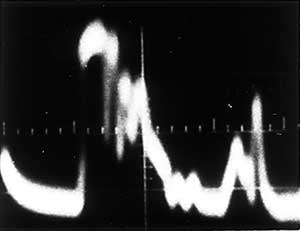
\includegraphics[height=4cm, width=\textwidth]{A-Mode}  
  	\caption{A-Mode}
  	\label{fig:a_mode}
  \end{subfigure}
  \hfill
  \begin{subfigure}[b]{0.48\textwidth}
	\centering
  	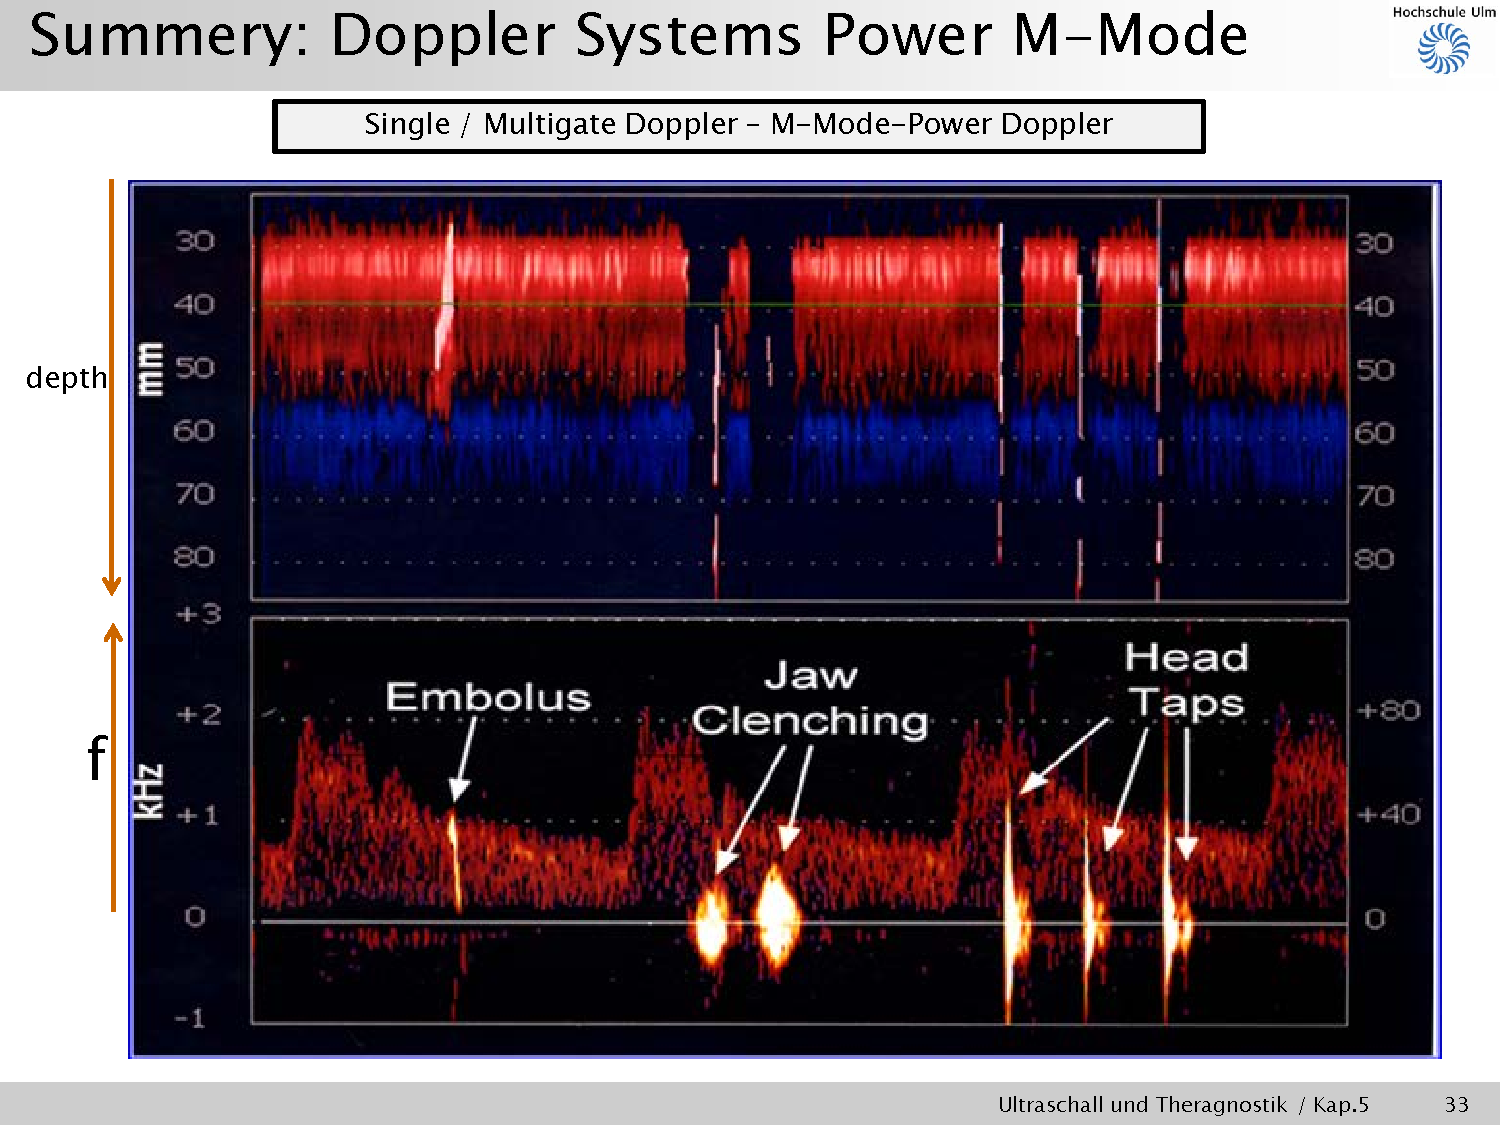
\includegraphics[trim = 2.2cm 1cm 1.3cm 3.5cm, clip=true,height=4cm, width=\textwidth]{M-Mode}  
  	\caption{M-Mode mit Doppler Spektrogram}
  	\label{fig:m_mode}
  \end{subfigure}
  \caption{Modes der Bildentstehung}
  \label{fig:modes}
\end{figure}
\newpage
\section{Methoden der Emboliedetektion}
blablabla
\end{comment}


\chapter{Material und Methode}
\section{Material}
\subsection{Verwendete Programme}
%\subsubsection*{Eagle}
%\href{http://www.cadsoft.de/?language=de}{Cadsoft Eagle} ist eine \ac{pcb} Design Software, welche für Microsoft\SymbC Windows\SymbReg, Linux Distributionen sowie für Apple OS X verfügbar ist und aktuell die Versionsnummer 6.5.0 trägt. Diese Software wurde für die Erstellung eines Schaltplans, sowie für das Erstellen eines Leiterplattenlayout genutzt, was sich durch die Ableitung des zuvor erstellten Schaltplans schnell realisieren lies. Dazu stehen der Schaltplan-Editor und der Layout-Editor zur Verfügung, welche sich gegenseitig synchronisieren und Änderungen in dem jeweils anderen Editor sichtbar machen. Die Überprüfung des Leiterplattenlayout durch "Design Rules", welche man bei den gewünschten Hersteller der Platinen beziehen kann, wird bereitgestellt, wodurch die Entwicklungszeit und Fehler reduziert werden. \cite{eagle}
\subsubsection*{Altium Designer}
\href{http://www.altium.com/de/altium-designer/overview}{Altium\SymbReg Designer\SymbReg} ist eine \ac{pcb} Design Software, welche für Microsoft\SymbC Windows\SymbReg verfügbar ist und aktuell die Versionsnummer 15.1.12 trägt. Diese Software wurde für die Erstellung eines Schaltplans, sowie für das Erstellen eines Leiterplattenlayout genutzt, was sich durch die Ableitung des zuvor erstellten Schaltplans schnell realisieren lies. Dazu stehen der Schaltplan-Editor und der Layout-Editor zur Verfügung, welche sich gegenseitig synchronisieren und Änderungen in dem jeweils anderen Editor sichtbar machen. Die Überprüfung des Leiterplattenlayout durch "Design Rules", welche man bei den gewünschten Hersteller der Platinen beziehen kann, wird bereitgestellt, wodurch die Entwicklungszeit und Fehler reduziert werden. \cite{altium}

\subsubsection*{LTspice IV}\label{sw:ltspice}
\href{LTspice IV}{LTspice IV\SymbReg} ist ein hochperformanter SPICE Simulator, welcher für Microsoft\SymbC Windows\SymbReg und Mac OS X 10.7+ verfügbar ist und aktuell die Versionsnummer 4.23e trägt. Diese Software wurde von Linear Technology Corporation für die analoge Schaltungssimulation entwickelt, wodurch Sie für die Validierung des Bandpassfilters sowie der Transmitteransteuerung genutzt werden konnte. \cite{ltspice}

\subsubsection*{Lattice Diamond}\label{subsub:diamond}
Diamond\SymbReg  ist eine Design Software der Firma Lattice\SymbC, welche für Microsoft\SymbC Windows\SymbReg und Linux Distributionen verfügbar ist. Diese wurde für die Erstellung von Logikmodulen (in der Programmiersprache Verilog 2.0) und die Verknüpfung der erstellten Module in einem System Design verwendet. Dieses Design konnte durch den integrierten Compiler für die Programmierung des Lattice MachXO2\SymbTM bereitgestellt sowie übertragen werden. Dabei wurde die Version 3.4.080 verwendet.
\subsubsection*{ALDEC Active-HDL}
Active-HDL\SymbTM ist eine Design Erstellungs- und Simulations-\ac{ide} für \ac{fpga}'s der Firma Aldec, welche für Microsoft\SymbC Windows\SymbReg verfügbar ist. Diese Software ist in Lattice Diamond\SymbReg integriert und wurde für die Simulation \ac{bzw} Synthese der Logikmodule und des System Designs des MachXO2\SymbTM genutzt. Die verwendete Version trägt die Nummer 9.3 und die Buildkennung 2744.sp1.09.4995.01.
%\subsubsection*{Visual Studio Ultimate}
%Visual Studio\SymbReg ist eine Software Entwicklungs \ac{ide} der Firma Microsoft\SymbC, welche unter Microsoft\SymbC Windows\SymbReg verfügbar ist. Diese \ac{ide} wird für die Code Dokumentation verwendet und bietet zusätzlich sehr gute Code Analyse Tools für die Programmiersprachen C, C++ und alle .NET Sprachen.
\subsubsection*{NXP Semiconductors LPCXpresso}\label{sec:xpresso}
\href{http://www.lpcware.com/lpcxpresso/home}{LPCXpresso} ist eine Software Entwicklungs \ac{ide} auf der Basis von Eclipse. Mit dieser Software wurde die Firmware des ARM-Cortex erstellt und gedebuggt. \cite{lpcxpresso}
\subsubsection*{Texmaker}
Bei \href{http://http://www.xm1math.net/texmaker/}{Texmaker} handelt es sich um ein Textsatzprogramm, welches von Pascal Brachet\SymbC unter Verwendung von Qt 5.2.1 sowie Poppler 0.26.5 compiliert wurde und für Microsoft\SymbC Windows\SymbReg, Linux Distributionen sowie für Apple OS X verfügbar ist. Die aktuelle Version, welche verwendet wurde trägt die Versionsnummer 4.4.1.
%\subsubsection*{Inventor}
%Als CAD-Programm wird Inventor\SymbReg Professional 2014 verwendet. Dieses, von Autodesk\SymbReg zur Verfügung gestellte Programm bietet Möglichkeiten zur Modellierung von 3D-Konstruktionen und Finite-Element-Berechnung (FEM). Es können Einzelteile, Baugruppen und technische Zeichnungen erstellt werden.
%\subsubsection*{GIMP}\label{material:gimp}
%Bei \href{http://http://www.gimp.org/}{GIMP (GNU Image Manipulation Program)} handelt es sich um ein kostenloses und freies Bildbearbeitungsprogramm. Es ist für Microsoft\SymbC Windows\SymbReg, Linux und Unix Distributionen sowie für Apple OS X und AmigaOS 4 verfügbar. Die aktuelle Version, welche unter Microsoft\SymbC Windows\SymbReg verwendet wurde trägt die Nummer 2.8.10. \cite{gimp}

\subsection{Verwendete Geräte und Evalkits}
\subsubsection*{LPCXpresso LPC4337 / OM13070 von NXP}
Das OM13070 von NXP ist ein Prototyping Board, das eine komplette Abstrahierung der low-level \ac{mcu} Befehle durch einen Online-Compiler mit sich bringt. Das Board besteht aus 2 Komponenten. Den eigentlichen asymmetrischen ARM-Cortex M4/M0 Chip LPC4337 der Firma NXP und einen Debugger Chip. Dazu gehören Funktionen wie \ac{spi}, I2C, UART, CAN, GPIO, PWM, \ac{adc}, \ac{dac}, sowie Ethernet und \ac{usb} OTG.\\
Durch den \ac{hal} in Kombination mit dem ARM \ac{cmsis} kann der entwickelte Programmcode nicht nur schneller, sondern auch auf alle ARM-Cortex Modelle von NXP übertragen werden\footnote{sofern diese die programmierten Funktionen unterstützen}.

\subsubsection*{Funktionsgenerator PM5139 von Philips (Flunke Corporation)}\label{sec:funktionsgen}
Für die Evaluierung der Messplatine wurde dieser Funktionsgenerator vorgesehen, welcher Testsignale erzeugt. Dieser unterstützt die Signalformen Gleichstrom, Sinus, Dreieck, Quadrat, Puls und Sägezahn und kann diese Signalformen mit einer Wiederholfrequenz von 0.1 mHz bis 20 MHz mit einer maximalen Spitzenspannung von 20 V generieren. Die Signale werden mit einer Präzision von 10-Bit generiert. \cite{flunkePM5139}

\subsubsection*{Digital Oscilloscope HMO3524 von HAMEG Instruments}\label{sec:oszi}
Mit dem Oszilloskop von HAMEG Instruments werden Signale graphisch dargestellt. Dieses Gerät bietet eine Abtastrate von 4 x 2 GigaSamples/Sekunde und visualisiert Signale bis 350 MHz. Die Vertikale Auflösung beträgt 8 Bit und im HighResolution Mode bis zu 10 Bit. Es besitzt 2 MB internen Speicher und zählt zu den Speicheroszilloskopen. Es bietet auch Funktionen im Bereich der Mathematik an, wie \ac{zb} eine \ac{fft} Analyse für die Darstellung der gemessenen Signalfrequenzen. Für die Dokumentation wird das Speichern von Bildern auf einen \ac{usb}-Stick oder über die mitgelieferte Software auf dem \ac{pc} bereitgestellt. \cite{hamegHMO}

\subsubsection*{Spectrum Analyzer FSL3 von Rohde \& Schwarz mit Schnüffelsonde}\label{sec:analyzer}
Mit dem Spektrumanalysator FSL3 von Rohde \& Schwarz werden Signale graphisch dargestellt. Dieses Gerät bietet eine Signalanalyse in Form einer Spektralverteilung für Frequenzen zwischen 9 \ac{khz} bis 3 \ac{ghz}. Somit kann das erfasste Signal in seine Einzelfrequenzen zerlegt werden. Es bietet zudem die Möglichkeit, 4 Marker für definierte Frequenzen zu setzen und somit den Leistungspegel dieser Frequenzen direkt zu visualisieren. Die minimale Frequenzauflösung beträgt dabei 1 Hz, was mehr als ausreichend für die Messung dieser Arbeit sind. Für die Dokumentation der Daten wird das Speichern von Bildern und der Rohdaten als ASCII-Werte auf einen \ac{usb}-Stick oder über die mitgelieferte Software auf dem \ac{pc} bereitgestellt. \cite{rohdeFSL3}\\
Eine Prüfsonde für elektrische und magnetische Wechselfelder, auch Schnüffelsonde genannt, wurde für die Lokalisierung von Signalstörungen auf der Platine genutzt. Dabei wurde die Schnüffelsonde mit einen \ac{lna} an den FSL angeschlossen. Diese arbeiten für elektrische Felder nach dem Prinzip der Ladungsverschiebung einer Kapazität, welche von der Feldstärke abhängt und für magnetische Felder nach dem Prinzip eines Strom-Spannungswandlers durch Induzierung einer Wechselspannung in eine Spule. Somit muss die richtige Sonde für die Messung von AC- und DC-Störungen ausgewählt werden.

\section{Methode}
Für das generieren des M-Mode (\ref{m-mode}) und des Doppler Spektrogramm (\ref{spektrogramm}) Graphen aus den digitalisierten Signalen der Ultraschallsonde muss eine Verarbeitung des Signales erfolgen. Dafür wird zunächst das Signal demoduliert und in den \ac{nf} Bereich transformiert. Anschließend findet ein Datentransfer statt, welcher durch einen parallelen Datentransfer realisiert wird. Nachdem die demodulierten Daten über den ARM-Cortex M4 an einen \ac{pc} transferiert wurden, muss eine \ac{fft} zur Darstellung des Doppler Spektrogramm als Audiosignal sowie als Graph erfolgen. In den folgenden Abschnitten werden die dafür benötigten Methoden detaillierter beschrieben, wobei für den parallelen Datentransfer eine 8-bit breite Schnittstelle als ausreichend erschien.
\subsection{Digitaler Hochpass}\label{sec_digHP}
Für die Optimierung des \ac{snr} ist ein digitaler Hochpass geplant. Grund dafür ist die Annahme, dass bei den differenziellen Eingangssignal Störungen unterhalb von 1 \ac{mhz} durch die Spannungsversorgung und kapazitiven Einkopplungen stattfinden, welche sich gleichmäßig\footnote{Common Mode} auf das Signal auswirken können. Zudem wird durch eine Vorverstärkung des Signals immer ein DC-Offset generiert, was bei den geringen Signalpegeln von mehreren $\mu$V bis wenigen mV das \ac{snr} extrem beeinflusst. Da ein passiver Hochpassfilter ein Eigenrauschen sowie ein Offset besitzt und die Steilheit der Amplitudenänderungen verringert, ist ein digitaler Hochpass nicht nur günstiger, sondern auch effektiver.\\
Grundlegend muss sich für eine Art der digitalen Filterung entschieden werden, wobei die \ac{fir} und \ac{iir} Filtertechnik zu Verfügung stehen. Da die Digitalisierung (Abtastrate $f_A$) mit 64 \ac{mhz} durchgeführt wird und Signale mit Frequenzen unterhalb von 500 \ac{khz} als Störungen angesehen werden, muss das Filter im \ac{cpld} abgebildet werden, was die Nutzung von Multiplikationen stark einschränkt, um die Taktfrequenz der Logikeinheit nicht zu stark zu belasten. Daher wurde sich für die einfachste Art von digitalen Filter entschieden - einen \ac{fir} Filter mit Multiplikatoren von 1 wodurch Multiplikationen entfallen. Dabei benötigt das Filter 128+1 Verzögerungen / Speicherelemente, da 
\[\dfrac{64.000\ \ac{khz}}{500\ \ac{khz}}=128\ Elemente\]
Die Realisierung wird durch ein 128 Elemente Tiefes Schieberegister ermöglicht, was pro Takt die digitalisierten Werte weiter schiebt. Dabei wird der letzte Wert im Schieberegister mit den Kehrwert des neuen Wertes multipliziert und als Signal an die Demodulierung weitergereicht. Dabei entsteht eine zusätzliche Verzögerung von mindestens 3 Takten durch die Multiplikation, was jedoch bei der hohen Taktfrequenz und der kontinuierlichen Messung vernachlässigbar und somit kompensierbar ist.

\subsection{Digitaler Tiefpass}
Ein Digitaler Tiefpass wird für die Quadraturdemodulierung (\autoref{sec:demodulate}) benötigt, da die \ac{hf} Modulation eliminiert werden muss. Dabei nutzt man die Information, dass man mit einer Trägerfrequenz arbeitet, welche durch den Dopplereffekt um wenige \ac{khz} verschoben wird. Zudem ist die Periodenzahl der Trägerfrequenz im Burst definiert, wodurch die maximale axiale Auflösung $R_A$ bekannt ist.\footnote{$R_A=spatial\ pulse\ length\ (mm)/2$} Somit kann ein einfacher Tiefpass auf Basis des \ac{fir} Filtertechnik verwendet und realisiert werden.\\
Wenn eine durch 2 teilbare Anzahl von Perioden im Burst definiert wird, ist die maximale axiale Auflösung $Burst/2$ wodurch ein Addition über $Burst/2$ Perioden ausreichend ist und die optimale Informationsgröße beinhaltet. Dabei werden Messwerte eines definierten Zeitbereichs addiert, wodurch sich die positiven mit den negativen Werten eliminieren. Man spricht bei dieser Technik auch von moving average (Gleitender Mittelwert), da die Grundfrequenz \(f_0\) und deren grade Oberwellen eliminiert werden, wobei der \ac{nf} Anteil vorhanden bleibt. 

%
%
%
\subsection{Quadraturdemodulation}\label{sec:demodulate}
\begin{figure}[h!t]
\centering
\begin{tikzpicture}
	\matrix (m0) [row sep=2.5mm, column sep=12mm]
	{	%--------------------------------------------------------------------
		\node[coordinate]                  (m00) {};   		  &
		\node[coordinate]                  (m01) {};   		  &
		\node[dspmixer]                    (m02) {};   		  &
		\node[dspsquare]                   (m03) {LPF};   	  &
		\node[dspnodeopen,dsp/label=below] (m0X) {$I[n]$};	  \\				%--------------------------------------------------------------------
		\node[dspnodeopen,dsp/label=above] (m10) {$r[n]$};    &
		\node[dspnodefull]                 (m11) {};          &
		\node[coordinate]                  (m12) {};          &
		\node[coordinate]                  (m13) {};          &
		\node[coordinate]                  (m1X) {};          \\		%--------------------------------------------------------------------
		\\		%--------------------------------------------------------------------
		\node[coordinate]                  (m20) {};          &
		\node[coordinate]                  (m21) {};          &
		\node[dspmixer]                    (m22) {};   		  &
		\node[dspsquare]                   (m23) {LPF};		  &
		\node[dspnodeopen,dsp/label=below] (m2X) {$Q[n]$};    \\		%--------------------------------------------------------------------		%--------------------------------------------------------------------
		\node[coordinate] (m30) {}; &
		\node[coordinate] (m31) {}; &
		\node[coordinate] (m32) {}; &
		\node[coordinate] (m33) {}; &
		\node[coordinate] (m3X) {};    \\		%--------------------------------------------------------------------
	};	
	\begin{scope}[start chain]
		\chainin (m10);
		\chainin (m11) [join=by dspconn];
		\chainin (m01) [join=by dspline];
		\chainin (m21) [join=by dspline];
	\end{scope}
	\draw[dspconn]  (m12) -- node[below] {$cos(2\pi f_0n)$} (m02);	
	\draw[dspconn]  (m32) -- node[below] {$sin(2\pi f_0n)$} (m22);	
			
	\foreach \i [evaluate = \i as \j using int(\i+1)] in {1,..., 2}
	{
		\draw[dspconn] (m0\i) -- (m0\j);
		\draw[dspconn] (m2\i) -- (m2\j);
	}
	\draw[dspflow] (m03) -- (m0X);
	\draw[dspflow] (m23) -- (m2X);
\end{tikzpicture}
\caption{Blockdiagramm Quadraturdemodulation und Tiefpass}
\label{fig:demo}
\end{figure}

Die Quadraturdemodulation ist eine Möglichkeit, Hochfrequente Eingangssignale in den Niederfrequenzbereich umzuwandeln. Dabei wird das Eingangssignal \(r[n]\) mit der Trägerfrequenz \(f_0\) multipliziert.\\
Für die Digitale Umsetzung der Demodulierung benötigt man eine \ac{lut} mit Sinus- und oder Cousinuswerten sowie 2 Multiplizierer und 2 Addierer. Die \ac{lut} rotiert dabei mit der Trägerfrequenz $f_0$ oder einen vielfachen davon, je nachdem, wie viele Stützstellen in der \ac{lut} vorhanden sind. Dabei errechnet sich die Anzahl der \ac{lut} Stützstellen $N_S$ wie folgt:
\begin{equation}
N_S=\frac{f_{Sampling}}{f_0}\ mit\ N_S\in\mathbb{N}
\end{equation}
Es ist zu Beachten, dass die Anzahl der Stützstellen eine Ganze Zahl $\mathbb{N}$ ist. Somit sollte die Samplingfrequenz \(f_{Sampling}\) ein Vielfaches der Trägerfrequenz $f_0$ darstellen um Fehler der Berechnung zu vermeiden.\\
Durch die nachgestellte Addition des Realteils und des Imaginärteils werden die Summenfrequenzen der Multiplikation eliminiert. Diese Technik wird auch als \ac{fir} oder moving average Filter bezeichnet.
%
%
%
\subsection{\acl{spi}}\label{subsec:spi}
Das \ac{spi} ist ein Bus-System, welches von Motorola entwickelt wurde. Es besteht aus drei oder vier Signalleitungen und dient der seriellen, synchronen Datenübertragung zwischen einem Master und einem Slave (3-Wire Mode) oder einem Master und mehreren Slaves (3-/4-Wire Mode). \\
Die Signalleitungen des \ac{spi} setzen sich dabei wie folgt zusammen:
\begin{description}
\item[SCK (Serial Clock)] ist das Taktsignal, welches vom Master bereitgestellt wird.
\item[MOSI (Master Out, Slave In)] dient dem Master für die Datenweitergabe an den Slave. 
\item[MISO (Master In, Slave Out)] dient dem Master für den Empfang der Daten des selektierten Slaves.
\item[CS (Chip Select)] dient dem Selektieren des Slaves und ist low Aktiv.
\end{description}
\begin{figure}[h!t]
	\centering
  	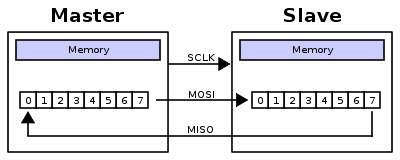
\includegraphics[width=0.5\textwidth]{SPI_8-bit_circular_transfer}
  	\caption{SPI Schieberegister Master-Slave}
  	\label{fig:SPI_Shift}
\end{figure}
Der Vorteil des \ac{spi} ist sein Vollduplex Modus, welcher durch Schieberegister in Slave und Master realisiert wird (siehe Abb. \ref{fig:SPI_Shift}). Für die Datenübertragung ergeben sich 4 verschiedene Modi, welche sich durch einstellen der \textit{Clock Polarity (CPOL)} und der \textit{Clock Phase (CPHA)} ergeben (siehe Tab. \ref{tab:spi_modes}). 
\begin{figure}[h!]
\centering
\begin{tikztimingtable}[timing/d/background/.style={fill=white},
   timing/lslope=0.2]
          CPOL=0 & LL 15{T} LL \\
          CPOL=1 & HH 15{T} HH \\
                 & H 17L H     \\
  \\
        Cycle \# & U     R 8{2Q} 2U    \\
            MISO & D{z}  R 8{2Q} 2D{z} \\
            MOSI & D{z}  R 8{2Q} 2D{z} \\
  \\
        Cycle \# & UU    R 8{2Q} U    \\
            MISO & D{z}U R 8{2Q} D{z} \\
            MOSI & D{z}U R 8{2Q} D{z} \\
\extracode
  % Add vertical lines in two colors
  \begin{pgfonlayer}{background}
    \begin{scope}[semitransparent,semithick]
      \vertlines[red]{2.1,4.1,...,17.1}
      \vertlines[blue]{3.1,5.1,...,17.1}
    \end{scope}
  \end{pgfonlayer}
  % Add big group labels
  \begin{scope}
    [font=\sffamily\Large,shift={(-6em,-0.5)},anchor=east]
    \node at (  0, 0) {SCK};    \node at (  0,-3 ) {CS};
    \node at (1ex,-9) {CPHA=0}; \node at (1ex,-17) {CPHA=1};
  \end{scope}
\end{tikztimingtable}
\caption{\ac{spi} Datenübertragung mit unterschiedlichen Einstellungen}
\end{figure}
\begin{table}[h!]
\centering
\caption{\ac{spi} Modi Einstellungen}
\label{tab:spi_modes}
\begin{tabular}{c|c|c}
\textbf{Mode} & \textbf{Clock Polarity} & \textbf{Clock Phase} \\
\cline{1-3}
0	& 0	& 0 \\ 
1	& 0	& 1 \\ 
2	& 1	& 0 \\ 
3	& 1	& 1 \\ 
\end{tabular}
\end{table}
%
%
%
\subsection{paralleles Dateninterface}\label{subsec:interface_parallel}
Für die Realisierung eines parallelen Dateninterfaces wird mindestens eine Datenleitung, welche die eigentliche Information des Bits enthält, sowie eine Taktleitung, welche den Schreibbefehl initialisiert, benötigt. Dabei kann die Anzahl an Datenleitungen variieren. In diesem Layout wurde sich für ein 8-bit breites Interface entschieden, da dieses mit einen Clock von 16 \ac{mhz} betrieben werden soll. Somit könnte eine theoretische Datenrate von 16 MB/s\footnote{$16\cdot 10^6$ Byte} realisiert werden, was zwar nicht die theoretischen 60 MB/s\footnote{480 mbit/s} der High-Speed \ac{usb} 2.0 Schnittstelle ausreizt, jedoch 160 32-Bit Werte bei einer \ac{prf} mit 12 \ac{khz} übertragen kann. Somit kann die Datenrate um 400 \% in Bezug auf die vorangestellte Arbeit gesteigert werden und bietet durch eine Busverbreitung auf 16 bit eine theoretische Datenrate von 32 MB/s.\\
%Serienwiderstände für die Reduzierung des Ringings wurden bei dieser Übertragungsfrequenz vernachlässigt.
Für die Synchronisierung der Daten wurde sich der Technik der PAL video Synchronisierung bedient. Dabei handelt es sich um ein zusätzliches Signal, welches den Spannungspegel bei Übertragung eines Pakets ändert. Mit dieser Technik können die übertragenen Werte einer \ac{prf} zugeordnet werden, was dem Empfänger die weitere Verarbeitung der Werte erleichtert. Somit entfällt eine sonst notwendige Nachbearbeitung durch Zuordnung von Start- und Stopbits des Transfers. Diese Erweiterung reduziert die \ac{mcu} Last des Empfängers, wodurch diesem mehr Zeit für andere Aufgaben \ac{resp} Berechnungen zu Verfügung stehen.
%
%
%
\newcounter{wavenum}

\setlength{\unitlength}{1cm}
% advance clock one cycle, not to be called directly
\newcommand*{\clki}{
  \draw (t_cur) -- ++(0,.3) -- ++(.5,0) -- ++(0,-.6) -- ++(.5,0) -- ++(0,.3)
    node[time] (t_cur) {};
}

\newcommand*{\bitvector}[3]{
  \draw[fill=#3] (t_cur) -- ++( .1, .3) -- ++(#2-.2,0) -- ++(.1, -.3)
                         -- ++(-.1,-.3) -- ++(.2-#2,0) -- cycle;
  \path (t_cur) -- node[anchor=mid] {#1} ++(#2,0) node[time] (t_cur) {};
}

% \known{val}{length}
\newcommand*{\known}[2]{
    \bitvector{#1}{#2}{white}
}

% \unknown{length}
\newcommand*{\unknown}[2][XXX]{
    \bitvector{#1}{#2}{black!20}
}

% \bit{1 or 0}{length}
\newcommand*{\bit}[2]{
  \draw (t_cur) -- ++(0,.6*#1-.3) -- ++(#2,0) -- ++(0,.3-.6*#1)
    node[time] (t_cur) {};
}

% \unknownbit{length}
\newcommand*{\unknownbit}[1]{
  \draw[ultra thick,black!50] (t_cur) -- ++(#1,0) node[time] (t_cur) {};
}

% \nextwave{name}
\newcommand{\nextwave}[1]{
  \path (0,\value{wavenum}) node[left] {#1} node[time] (t_cur) {};
  \addtocounter{wavenum}{-1}
}

% \clk{name}{period}
\newcommand{\clk}[2]{
    \nextwave{#1}
    \FPeval{\res}{(\wavewidth+1)/#2}
    \FPeval{\reshalf}{#2/2}
    \foreach \t in {1,2,...,\res}{
        \bit{\reshalf}{1}
        \bit{\reshalf}{0}
    }
}

% \begin{wave}[clkname]{num_waves}{clock_cycles}
\newenvironment{wave}[3][Dataclock]{
  \begin{tikzpicture}[draw=black, yscale=.7,xscale=1]
    \tikzstyle{time}=[coordinate]
    \setlength{\unitlength}{0.5cm}
    \def\wavewidth{#3}
    \setcounter{wavenum}{0}
    \nextwave{#1}
    \foreach \t in {0,1,...,\wavewidth}{
    %  \draw[dotted] (t_cur) +(0,.5) node[above] {t=\t} -- ++(0,.4-#2);
      \clki
    }
}{\end{tikzpicture}}


\begin{figure}[h!]
\centering
\begin{wave}{3}{5}
 \nextwave{Dataline[0\ldots 7]}	\bit{0}{0.5} \known{}{1}\known{}{1}\known{}{1}\known{}{1}\known{}{1} \bit{0}{0.5}
 \nextwave{Dataframe} 		\bit{0}{0.5} \bit{1}{5} \bit{0}{0.5}
\end{wave}
\caption{Datenübertragung eines Frames mit der parallelen Schnittstelle}
\end{figure}

%
%
%
\subsection{Fast Fourier Transformation}
Die \ac{fft} ist eine Methode, welche Daten aus dem Zeitbereich in den Frequenzbereich überführt.\newline
Diese Methode beruht auf einen Algorithmus, welcher die Eingangswerte vertauscht. Dabei wird in jedem Schritt das Abtastintervall zwischen zwei Werten verdoppelt. Dies wird solange wiederholt, bis alle Eingangswerte in 2-er Gruppen gespaltet sind. Dies hat zur Folge, dass für die \ac{fft} immer ein ganzzahliges vielfaches der Auflösungsfrequenz korrekt ermittelbar ist.\newline
Die \ac{dft} benötigt \textbf{$N^2$} und die \ac{fft} \textbf{$N*log_{2}(N)$} Berechnungen. Somit werden für einen Zeitbereich von \ac{zb} $10^9$ ns für die \ac{fft} $\approx 30$ s und die \ac{dft} $\approx 31.2$ Jahre benötigt. \newline
Aus der Anzahl $N$ der Punkte und der Abtastfrequenz $f_A$ ist der Linienabstand im Frequenzbereich mit $\dfrac{f_A}{N}$ berechenbar. Weiterhin ist zu beachten, dass die \ac{fft} spiegelsymmetrisch zur Mitte ist und somit nur die Frequenzen von $k=0$ bis $k=\frac{N}{2}$ betrachtet werden und die k-te Frequenz $f_k$ durch $f_k=f*\dfrac{f_A}{N}$ definiert ist.

\chapter{Systemdesign und Implementierung}
\section{Systemübersicht}
\begin{figure}[!h]
	\centering
   	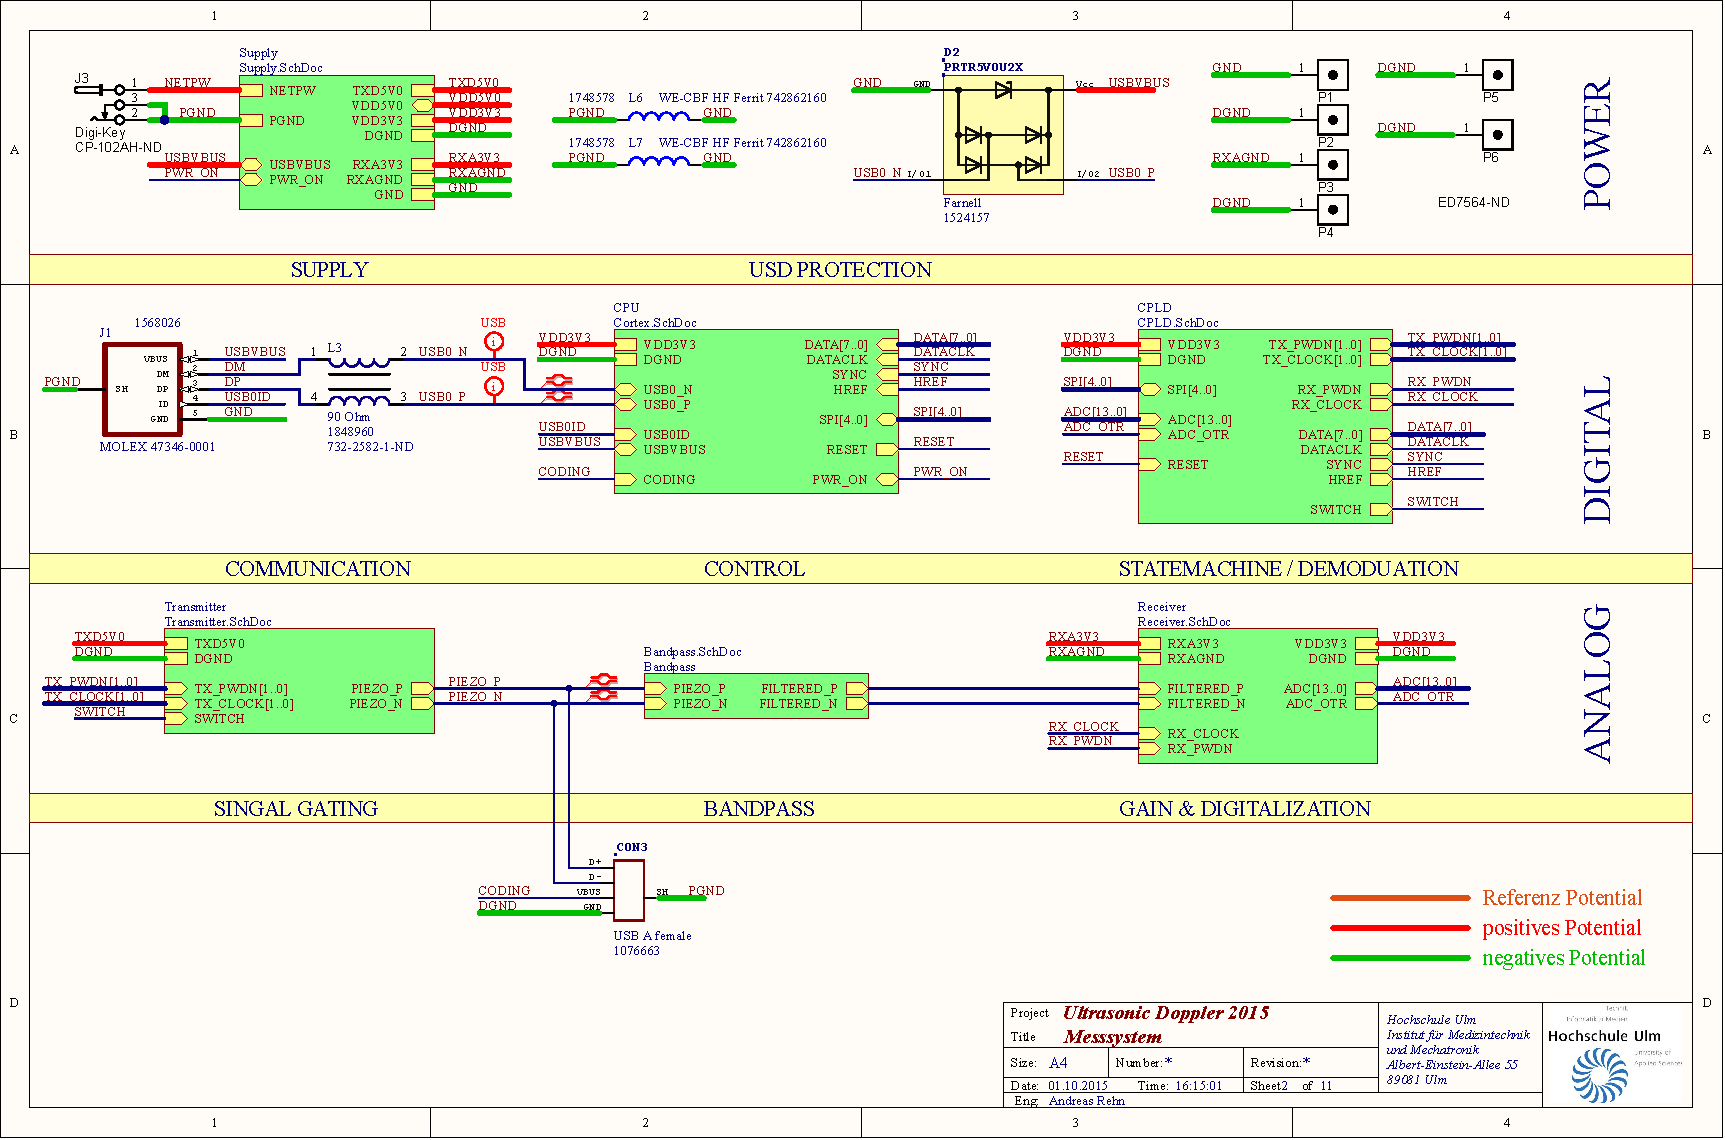
\includegraphics[page=1,width=1.0\textwidth, trim= 5mm 5mm 5mm 5mm, clip=true]{images/pcb/new.PDF}%docu
    \caption{Modulübersicht des Systems ohne mechanische und externe Komponenten}
    \label{fig:system}
\end{figure}
In diesem Kapitel wird das erstellte System und dessen Module näher beschrieben. Dabei wird das System in Analog, Digital, Power und mechanische Komponenten untergliedert.
\begin{itemize}
\item Um das System mit Energie zu versorgen wird eine Stromquelle benötigt, welche in \autoref{sec:supply} beschrieben wird. Da das System für die medizinische Anwendung konzipiert ist, wird zudem die Einspeisung des Systems und des \ac{pc}s des Benutzers beschrieben. Diese Beschreibung ist notwendig, da die Spannungsversorgung des Systems auf dem Verhalten der Einspeisung aufbaut.
\item Das Modul Analog beinhaltet dabei den Transmitter, welcher das zu emittierende Signal generiert, sowie den Receiver, welcher aus einen Bandpassfilter, einer \ac{lna} und einer Digitalisierung besteht.
\item Das Modul Digital beinhaltet hingegen die Ansteuerung des Transmitters und des Receivers sowie die Demodulierung und den Datentransfer zwischen dem System und den \ac{pc} des Nutzers.
\item Das Modul Gehäuse wurde aus der Übersicht entfernt, da dieses das gesamte Messsystem beinhaltet und nur die Schnittstellen für die Anbindung der Sonde, des \ac{pc}s sowie der Stromversorgung zur Verfügung stellt. Aus diesem Grund wurde das Gehäuse zwar vorgesehen, jedoch geht dieses in der aktuellen Entwicklungsphase nicht in die Implementierung des Systems ein.
\end{itemize}
Nachfolgend werden die genannten Module mit Spannungsversorgung, Kommunikation, Steuerung / Demodulierung, der Transmitter, der Receiver mit Bandpass sowie das Gehäuse näher betrachtet sowie erklärt. Zudem werden Aussagen über die Auslegung und die Realisierung dieser Module getroffen um den Leser ein besseres Verständnis des Systems und dessen Umsetzung zu geben.
\section{Spannungsversorgung}\label{sec:supply}
Damit das System arbeiten kann, benötigt das System elektrische Energie welche typischerweise von Außen zugeführt wird. Da der Fokus dieser Arbeit nicht auf der Energieversorgung des Dopplersystems liegt, wurde als Ausgangsbasis ein externes Schaltnetzteil der Firma SL Power Electronics verwendet, welches bei 230 V AC Netzspannung ein 19 V DC Ausgangsspannung mit 3,1 A liefert. Zudem ist das Netzteil GXM60-19A04 nach EN60601 geprüft und somit für medizinische Anwendungen zugelassen. Versionen für den internen Einbau sind dabei im Bereich von 5 bis 56 V DC beziehbar.\\%http://www.slpower.com/products/internal-medical-power-supplies/overview.html
Um elektromagnetische Störungen im System möglichst gering zuhalten, wurden Potentiale anhand der Arbeitsbereiche der elektronischen Komponenten bestimmt, festgelegt und gruppiert. Dabei ergab sich ein Potential für die digitale Signalverarbeitung, ein separiertes Potential für die analoge Signalverarbeitung sowie ein Potential für die Ansteuerung des Piezoelementes. Für die Potentiale wurden folgende Spannungen - 5 V DC \textit{TXD5V0} für die Piezoelementansteuerung, 3,3 V DC \textit{RXA3V3} für die analoge Signalverarbeitung und 3,3 V DC \textit{VDD3V3} für die digitale Signalverarbeitung - definiert.\\
Für die elektrische und mechanische Verbindung zwischen externen Schaltnetzteil und dem System wurde eine DC Power Jack Buchse gewählt, da das Netzteil geprüft ist und somit nicht veränderbar ist, ohne folgende Prüfungen und somit Kosten zu verursachen. Dabei ist bekannt, dass es zu Fehlbedienungen durch den Nutzer kommen kann, indem dieser Netzteile mit vertauschter Polung und oder Netzteile mit zu hohem Spannungsbereich nutzt. 
Für den Verpolungsschutz wurde ein kostengünstiger P-\ac{mosfet} genutzt, welcher nur durchschaltet, wenn das richtige Spannungspotenzial anliegt. Dieser limitiert gleichzeitig die minimale und maximale Spannung des Eingangs durch seinen Arbeitsbereich von \ac{ca} -0,55 V  bis -20 V DC. Dieser dient gleichzeitig als \textit{schwächstes} Bauelement, wenn der maximale Spannungsbereich überschritten wird, was die Fehlersuche beträchtlich einschränkt und folgende Komponenten schützt. Jedoch muss der \ac{mosfet} anschließend ausgetauscht werden.\\
Da das System auch über eine \ac{usb} Verbindung verfügt, kann das System theoretisch über eine \ac{usb} 2.0 Verbindung eine Spannung von 5 V DC mit einen maximalen Strom von 500 mA beziehen. Jedoch schwankt die unregulierte Spannungsversorgung je nach Quelle (\ac{zb}Laptop / \ac{pc}) von 4,75 V DC bis 5,5 V DC was für das Potential der Piezoelementansteuerung als nicht nutzbar erscheint. Zudem ist die erhöhte Stromaufnahme von 400 mA des Transmitters (\autoref{sec:transmitter}) nicht sichergestellt, wenn ein \ac{usb}-Hub oder mehrere Geräte an den \ac{pc} oder Laptop angeschlossen sind. Somit wurde eine Versorgung des Transmitters über \ac{usb} ausgeschlossen, jedoch können die analoge und die digitale Signalverarbeitung mit dieser Versorgung betrieben werden, was in dieser Phase der Entwicklung sinnvoll erscheint.
\subsection*{19 V DC zu 5 V DC}
Wie in \autoref{sec:transmitter} beschrieben, wird eine 5 Volt DC Spannung und ein 400 mA Strom für die Ansteuerung des Piezoelementes benötigt, damit ein Strom-Spannungswandler das zu emittierende Signal an die Amplitude des Piezoelementes anpassen kann. Um die benötigte Spannungspotential von 5 V DC zu genieren wurde der step-down (buck) Konvertierer MIC4680 der Firma MICREL genutzt, welcher einen maximalen Ausgangsstrom von 1,3 A liefern kann. Dieser arbeitet mit einer festen Frequenz von 200 \ac{khz} und besitzt einen Überstromschutz sowie eine automatische Abschaltung bei Übertemperatur.\\
Zudem wurde ein \ac{emi} Filter ausgelegt, welcher laut Simulation bei 75 \ac{khz} eine Dämpfung von -16 dB besitzt. Somit sollte eine ausreichende Dämpfung vorhanden sein, um die Oberwellen des Schaltreglers zu filtern und nicht in das Netz bzw. an das Netzteil einzukoppeln. Gleichzeitig kann durch dieses Filter eine Störfestigkeit gegen einstrahlende Frequenzen erreicht werden. % mit einer Dämpfung von -40 dB ab \ac{ca} 1 \ac{mhz}.
Da ein Schaltregler ein erhöhtes Rauschen aufweist, ist die Ausgangsspannung selbst durch Siebung und Glättung mit einen Kondensator nicht ideal für die Ansteuerung des Piezoelementes. Daher ist ein ADP7104 \ac{ldo} der Firma Analog Devices mit 550 mV dropout bei 500 mA vorgesehen, welcher ein Rauschen von 15 $\mu$V rms aufweist. Somit besteht die 5 Volt DC Generierung aus einen step-down, welcher die 19 V DC auf ein \ac{ca} 6,5 V DC Potenzial konvertiert mit einen nachgeschalteten \ac{ldo}. Somit kann eine Reduzierung der thermischen Belastung der Platine erreicht werden, was zudem auch den realen Leistungsbedarf senkt.\\
Parallel zu der Transmitterversorgung ist der analoge Leistungsschalter TPS2115A der Firma Texas Instruments verbaut, welcher automatisch die Stromversorgung der analogen und digitalen Signalverarbeitung von \ac{usb} auf das externe Netzteil schaltet, wenn Dieses angeschlossen ist. Somit kann sichergestellt werden, dass die \ac{pc} Software den aktuellen Stand des Systems an den Nutzer aufbereitet wiedergeben kann.
\subsection*{5 V DC zu 3,3 V DC analog}
Bei mixed-Signal \ac{pcb} Layouts muss auf Stromschleifen geachtet werden. Zudem wurde sich dafür entschieden, dass die Potenziale für die analoge und digitale Signalverarbeitung getrennt werden, was unterschiedliche Masseflächen mit Sternpunktverbindung zur Folge hat. Zudem war bei Erstellung des Layouts die maximale Taktfrequenz der analogen Komponenten durch die Digitalisierung mit 64 \ac{msps} limitiert.\\
Um die \ac{ic}s der analogen Signalverarbeitung zu stabilisieren sowie voneinander zu entkoppeln wurde jeweils ein Tiefpass 2. Ordnung vorgesehen. Dieser besitzt einen parallel geschalteten Pufferkondensator, welcher den Strom schnell an das Bauelement abgeben kann, und eine in Reihe geschaltete Spule, welche den Strom für die Aufladung des Kondensators begrenzt. Dadurch wird der \ac{ldo} weniger dynamisch belastet, wodurch ein stabiler Spannungspegel sichergestellt werden kann. Für die Generierung der 3,3 V DC Spannung wurde der \ac{ldo} ADP151 der Firma Analog Devices gewählt, da dieser 200 mA bei einen Spannungsripple von 9 $\mu$V rms liefern kann. Somit ist dieser ideal geeignet für die Versorgung der analogen Bauelemente.
%
%ref auf münzner
%
\subsection*{5 V DC zu 3,3 V DC digital}
Für die Versorgung des \ac{cpld}s und des ARM\SymbReg Cortex\SymbReg-M wurde der \ac{ldo} ADP7104 der Firma Analog Devices verwendet. Dieser liefert 500 mA bei einen Spannungsripple von 15 $\mu$V rms.
\newpage
\section{Transmitter}\label{sec:transmitter}
%scr0004 -> 10 Ohm Last
%scr0006 -> 8 Ohm Last
%scr0007 -> 6 Ohm Last
\newpage
\section{Entkopplung Transmitter Receiver}
Um das Verhalten von Transmitter und Receiver zu Entkoppeln wurden antiparallele Dioden (BAT64-04) verwendet. Die Durchbruchspannung dieser Dioden liegt bei 40 Volt, welche weder vom Trägersignal, noch vom empfangen Signal erreicht werden. Somit können die Dioden als Richtungsbegrenzer angesehen werden und das Verhalten kann für die Entkopplung genutzt werden. Ab 0,3 Volt Vorwärtsspannung hingegen werden diese leitend \ac{bzw} weisen diese ein niederohmiges Verhalten auf, woraufhin die Spannung durch die Anordnung der Dioden auf rund $\pm$ 0,3 Volt limitiert wird.\cite{bat64}
\begin{description}
\item[Senden des Signals:] Um den Receiver bei der Übertragung des Burstsignals durch die hohen Amplituden nicht zu zerstören wird das niederohmige Verhalten antiparalleler Dioden genutzt. Dabei sieht das Netzwerk einen niederohmigen Verbraucher, wodurch mögliche Ströme primär über die Dioden fließen und der Spannungspegel auf rund $\pm$ 0,3 Volt begrenzt wird. Je nach Positionierung im Netzwerk können Bauelemente und deren Verhalten verwendet oder terminiert werden. In dieser Arbeit wurden die antiparallelen Dioden nach den Induktivitäten des Bandpassfilters des Receiver Moduls positioniert, wodurch die Breitbandigkeit der Sonde gesteigert wird.
\item[Empfang des Signals:] In dieser Phase soll das Netzwerk nur den Receiver sehen. Da mit Empfangssignalen zu rechen ist, die kleiner $\pm$ 0,3 Volt sind, kann der Transmitter durch eine Serienschaltung der antiparallelen Dioden entkoppelt werden. Aus diesen Grund kann ein Widerstand zwischen Transmitter und den Dioden genutzt werden, um die Ausschwingzeit des Kristalls zu reduzieren, jedoch das Signal nicht beim Empfang belastet.
\end{description}
\begin{figure}[!h]
        \centering
        \begin{subfigure}[b]{0.48\textwidth}
        \centering
                \includegraphics[page=11, width=0.8\textwidth, trim =242mm 80mm 10mm 87mm, clip=true]{images/pcb/docu.pdf}
	    		\caption{im Ausgang der Transmitterschaltung}
	    		\label{fig:dioden_tx}
        \end{subfigure}%
        \hfil
        ~ %add desired spacing between images, e. g. ~, \quad, \qquad, \hfill etc.
          %(or a blank line to force the subfigure onto a new line)
        \begin{subfigure}[b]{0.48\textwidth}
                \includegraphics[page=3, width=\textwidth, trim=50mm 91mm 150mm 59mm, clip=true]{images/pcb/new.pdf}
		    \caption{im Bandpassfilter der Recieverschaltung}
		    \label{fig:dioden_rx}
        \end{subfigure}
        \caption{Anordnung der Dioden}\label{fig:filter_final}
\end{figure}
\newpage
\section{Receiver}\label{sec:receiver}
Der Receiver dient für den Empfang der \ac{rf} Signale sowie deren analogen Aufbereitung, damit diese Signale ideal digitalisiert werden können.\\
Dabei besteht das Receiver Modul des Systems aus einen differenziellen analogen Bandpass 2. Ordnung für die grundlegende Rauschminimierung der eingekoppelten und unerwünscht generierten Signale, einen Vorverstärker, welcher die gefilterten Signalamplituden an den Eingangsbereich des \ac{adc} Wandlers anpasst, sowie einen nachfolgenden \ac{adc} Wandler mit vorgeschalteter Impedanzanpassung.\\
In diesem Kapitel werden die einzelnen Abschnitte des Receiver Moduls näher beschrieben.
\subsection{Analoger Bandpass}
Wie in \autoref{sec:receiver} beschrieben, wird ein analoger Bandpass benötigt, um unerwünschte Signale zu dämpfen und somit das Rauschen zu minimieren. Dafür musste das Arbeitsfrequenzband definiert und der analoge Bandpass beschrieben werden.\\
Da das Arbeitsfrequenzband des Filter grundsätzlich beschreibt, werden die zu emittierenden Frequenzen (2, 4, 8 \ac{mhz}) in die Charakteristik einbezogen. Des weiteren soll der Dopplereffekt genutzt werden, welcher in \autoref{sec:dopplereffekt} auf Seite \pageref{sec:dopplereffekt} beschrieben ist. Dabei ist zu beachten, dass die Frequenz des emittierten Signales um bis zu \ac{ca} $\pm$ 10 \ldots 20 \ac{khz} verschoben werden kann. Außerdem muss beachtet werden, dass der Burst bei längerer Laufzeit einer erhöhten Dämpfung unterliegt. Somit muss das zeitliche Verhalten der emittierten Welle genauer betrachtet werden, da Reflektionen an Impedanzänderungen bzw. Dichteänderungen (Zellwände) auftreten und ein statisches Echo, also eine Reflektion ohne Frequenzänderung, zur Folge haben. Des weiteren unterliegt das Ein- und Ausschwingverhalten des Piezoelementes physikalischen Regeln, welche exponentiell sind\textbf{[REF!]}. Somit wird durch das Verhalten des Piezoelements das Trägersignal niederfrequent überlagert, was sich durch die \ac{prf} zyklisch wiederholt. Auch kann nicht ausgeschlossen werden, dass Oberwellen des Trägersignals gebildet und reflektiert werden. Da gerade Oberwellen durch den nachgestellten digitalen \ac{fir} Tiefpassfilter eliminiert werden können sind diese vernachlässigbar. Jedoch können ungerade Oberwellen ein summarischen Offset bei der Demodulierung erzeugen, welche die Messwerte verfälschen können. Dieses Verhalten gilt für alle Trägerfrequenzen.\\
Aus den oben genannten Fakten ist zu schlussfolgern, dass eine Hoch- und eine Tiefpass benötigt wird, um das Breitbandrauschen zu reduzieren und die Trägerfrequenzen mit dessen Dopplerschiebefrequenzen ungedämpft passieren zu lassen. Dabei sollte ein Hochpass für das Ausschwingverhalten des Piezoelementes und ein Tiefpass für die unerwünschten Oberwellen der Trägerfrequenzen dimensioniert werden.\\
Ein Bandpass zweiter Ordnung\footnote{40 dB/Dekade} wurde daher in Betracht gezogen, wobei die untere Grenzfrequenz $f_L$ auf 100 \ac{khz} und die obere Grenzfrequenz $f_H$ auf 8 \ac{mhz} festgelegt wurde. Zudem soll die minimale Dämpfung im Bereich von 2 \ac{mhz} liegen, da diese Trägerfrequenz die längste Laufzeit besitzt.
\subsection*{Implementierung}
Nachdem die Parameter des Filters definiert wurden, muss dieses mit realen Bauelementen umgesetzt werden. Dabei wurde eine Simulation der Schaltung mit der Software \nameref{sw:ltspice} durchgeführt, wodurch die Werte und somit die zu bestellenden \ac{smt} Bauteile bestimmt werden konnten.\\
Bei der Erstellung der Schaltung musste beachtet werden, dass das Signal differenziell eingespeist wird und der Eingangswiderstand des Vorverstärkers $R_{OAMP}=5\ k\Omega$ beträgt. Da der Innenwiderstand der 2, 4, 8 \ac{mhz} Sonden frequenzabhängig und nicht eindeutig deklariert ist, wurde dieser mit 50 $\Omega$ angenommen. Somit wurde die einfache Schaltung, welche in \autoref{fig:filter_half} deklariert ist erstellt.
\begin{figure}[!h]
	\centering
   	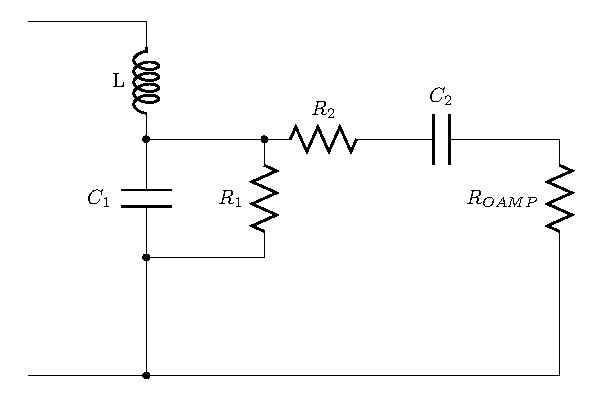
\includegraphics[width=0.48\textwidth]{images/Bandpass/half}
    \caption{vereinfachte Schaltung des Filters}
    \label{fig:filter_half}
\end{figure}\\
Dabei wurden für die Elemente L = 5.4 $\mu$H, $C_1$ = 47 pF, $R_1$ = 390 $\Omega$, $R_2$ = 24 $\Omega$ und $C_2$ = 235 pF bestimmt.
Diese Schaltung betrachtet jedoch nur eine Hälfte des Filters, wodurch die Werte für $L$ und $C_2$ der Schaltung wie folgt berechnet werden.
\begin{align*}
L=&\frac{L}{2}\\
C_2=&2\cdot C_2
\end{align*}
\clearpage
\begin{figure}[!h]
        \centering
        \begin{subfigure}[b]{0.48\textwidth}
                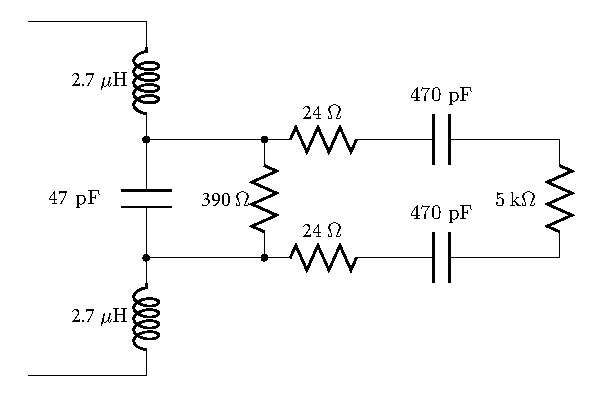
\includegraphics[width=\textwidth]{images/Bandpass/full}
	    		\caption{realisierbare Schaltung des Filters}
	    		\label{fig:filter_full}
        \end{subfigure}%
        ~ %add desired spacing between images, e. g. ~, \quad, \qquad, \hfill etc.
          %(or a blank line to force the subfigure onto a new line)
        \begin{subfigure}[b]{0.48\textwidth}
        	\includegraphics[width=\textwidth]{images/Bandpass/Bandpass}
		    \caption{Verhalten des Filters}
		    \label{fig:filter_verhalten}
        \end{subfigure}
        \caption{realisierbarer Filter}\label{fig:filter_final}
\end{figure}
Daraus ergibt sich die Schaltung aus \autoref{fig:filter_full}, welche mit beziehbaren Kaufteilen realisiert werden kann und dabei eine Filtercharakteristik nach \autoref{fig:filter_verhalten} aufweist. Dabei liegt die untere Grenzfrequenz $f_L$ bei 120 \ac{khz} und die obere Grenzfrequenz $f_H$ bei 13 \ac{mhz} wobei bei 1 \ac{mhz} die minimale Dämpfung von 0,1 dB vorherrscht.\\
Verstärkungen konnten jedoch im Bereich von 1,5 \ac{mhz} bis 10,5 \ac{mhz} erreicht werden.
\subsection{analoge Vorverstärkung}
Der Verstärkungsfaktor ist maßgeblich für das Signal-Rausch-Verhältnis und muss somit möglichst groß dimensioniert werden. Es wurde sich für einen differenziellen Verstärker von Analog Devices mit der Bezeichnung AD8351 entschieden\cite{ad8351}, bei dem die Verstärkung zwischen 0 und 26 dB justiert werden kann, was einen Spannungsverstärkung von 0 bis rund 20 mal dem Eingangssignal entspricht.\\
Damit der ideale Faktor bestimmt werden kann, wurde festgelegt, dass bei einen 50 $\Omega$ Eingangswiderstand ein Eingangssignal von 100 mVpp den gesamten Messbereich des 14-Bit \ac{adc}s abdeckt. Da der Eingangsbereich des \ac{adc}s auf 2 Vpp festgelegt ist, muss der Verstärkungsfaktor 20 betragen um den gesamten Bereich auszusteuern. Nach \autoref{fig:graph_gain} erkennt man, dass der differentielle Verstärker noch eine Dekade über der Nutzfrequenz konstant verstärkt. Daher muss der Lastwiederstand R$_L$ und der Verstärkungswiderstand R$_G$ näher betrachtet werden. Der \ac{adc} besitzt einen hochohmigen Eingang mit 7 k$\Omega$ wodurch ein Verstärkungswiderstand R$_G$ von 10 $\Omega$ oder kleiner benutzt werden sollte.
Da Bauelemente der E12 Reihe eine fertigungsbedingte absolute Toleranz von 5 $\%$ aufweisen, wurde sich für einen 8,2 $\Omega$ Widerstand für R$_G$ entschieden, um einen Verstärkungsfaktor von 20 zu erreichen.\\
Da jeder Verstärker ein Eigenrauschen aufweist und eine zu hohe Verstärkung das Signal-Rausch-Verhältnis verschlechtern kann, muss bei der Inbetriebnahme des gesamten Receiversmoduls der Verstärkungsfaktor für ein optimales Signal-Rausch-Verhältnis angepasst werden.
\begin{figure}[h!]
	\centering
	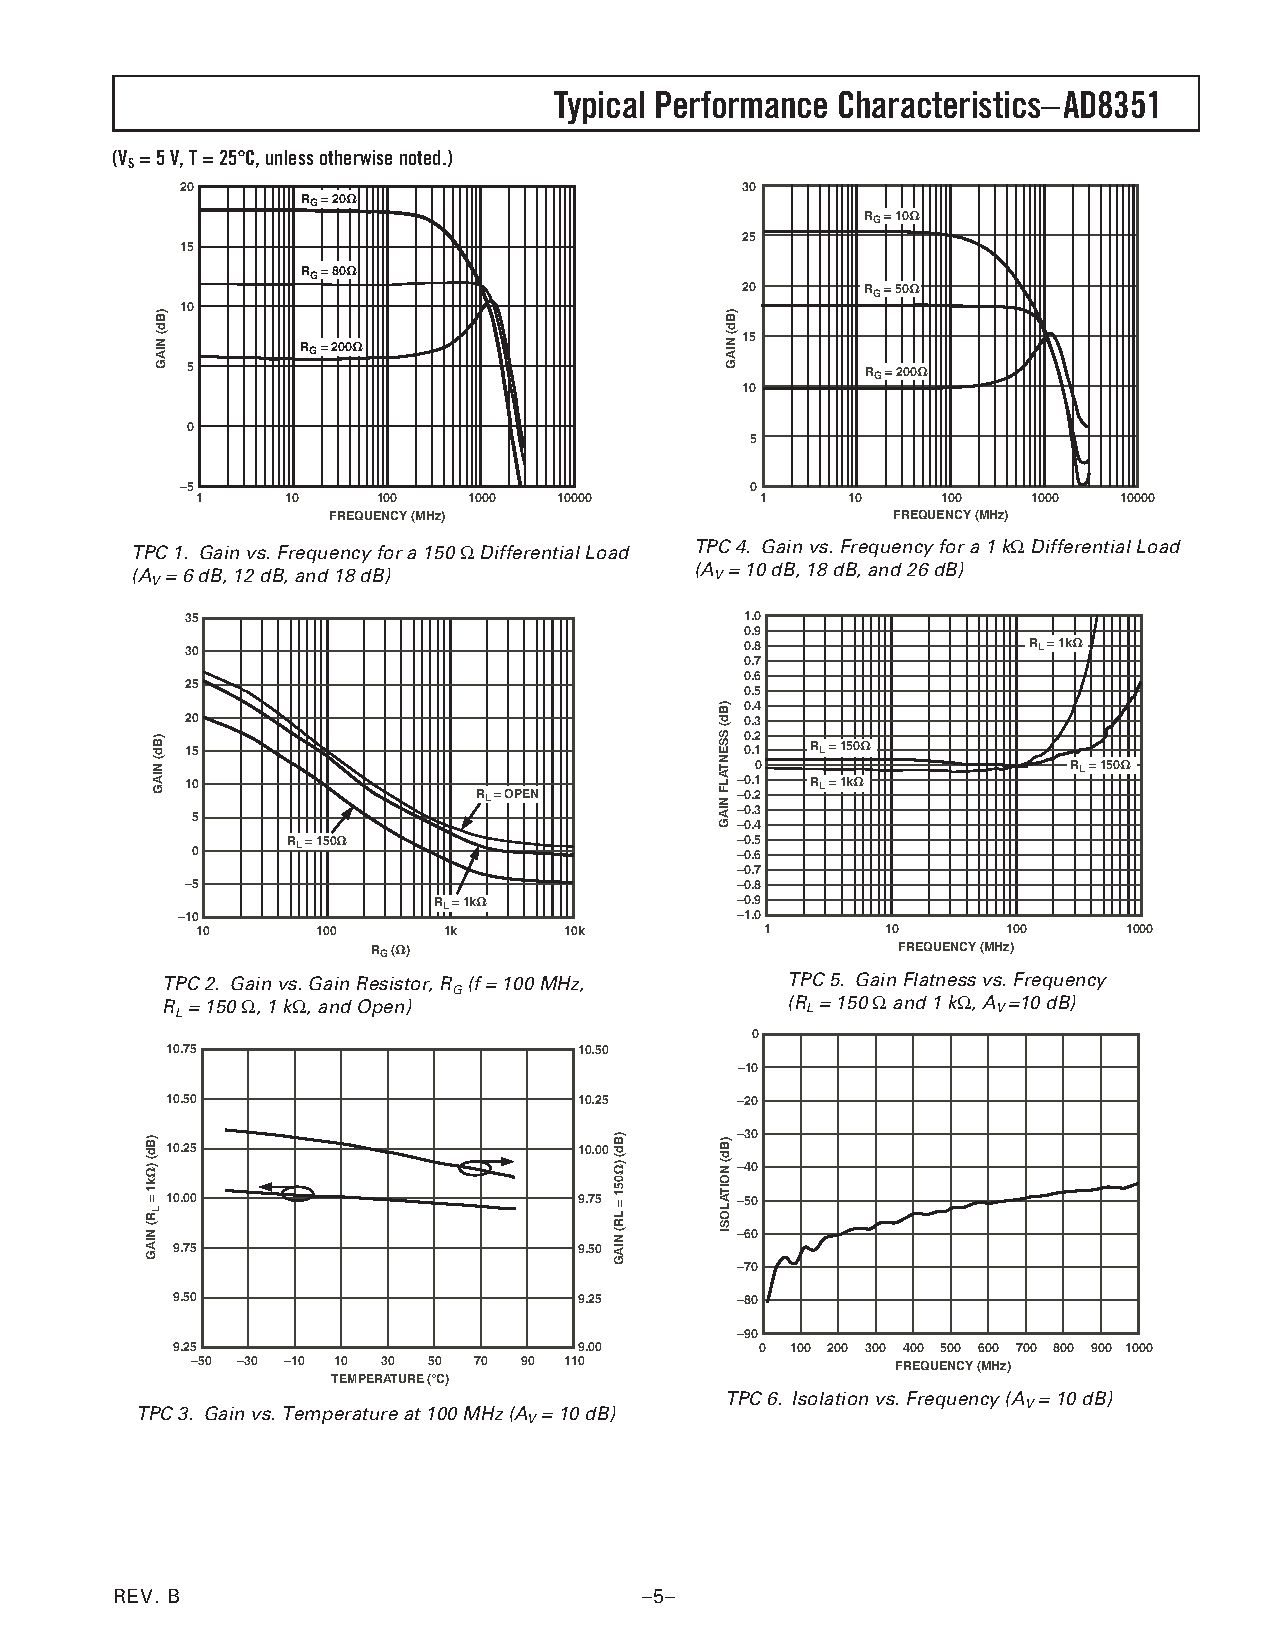
\includegraphics[width=1.0\textwidth, trim=20mm 180mm 15mm 30mm, clip=true]{images/Gain}
	\caption[Verstärkung in Abhängigkeit von Differenzieller Last, Frequenz und Verstärkungs-widerstand R$_G$]{Verstärkung in Abhängigkeit von Differenzieller Last, Frequenz und Verstärkungswiderstand R$_G$\cite[p. 7]{ad8351}}
	\label{fig:graph_gain}
\end{figure}
\newpage
\subsection{Digitalisierung}
Für die Diskretisierung des Signals und für dessen Weiterverarbeitung wird eine Analog-Digital-Wandlung benötigt. Da das Signal differenziell vorliegt, wurde der differenzielle \ac{adc} AD9245 der Firma Analog Devices verwendet, um die Vorteile des differenziellen Signals nicht zu verlieren.\cite{ad9245} \textbf{[REF! EMV / DIFF / SINGLE-ENDED]}\\
Dieser erzielte in den vorangegangen Arbeiten bereits ausreichende Messergebnisse. Dabei ist zu erwähnen das dieser 64 \ac{mhz} High-Speed \ac{adc} das Nyquistkriterium um ein 4-faches der maximalen Trägerfrequenz (8 \ac{mhz}) überschreitet. Dies wird wie in \textbf{[REF]} beschrieben für die Quadraturdemodulierung benötigt um eindeutige Aussagen über die Phase des Signals zu erhalten. Bei 4 Diskretisierungen pro Periode, also dem 2-fachen Nyquistkriterium, kann nicht garantiert werden, dass die maximale Auslenkung sowie die Nulldurchgänge digitalisiert werden, wodurch ein Quantisierungsfehler die Folge ist. Bei den Trägerfrequenzen von 2 und 4 \ac{mhz} kann zudem ein Oversampling mit 32 und 16 Diskretisierungen pro Periode erfolgen, wodurch für diese Frequenzen detailliertere Aussagen getroffen werden können.\\
Da auch in tieferen Blutgefäßen Aussagen über die Teilchengeschwindigkeiten getroffen werden müssen, wird eine hohe dynamic range benötigt, welche nur durch eine erhöhte Bitanzahl erzielt werden kann. Dabei wird folgende Formel mit der Bitanzahl N verwendet, um die Auflösung des \ac{adc}s zu erhalten, wobei positive sowie negative Amplituden digitalisiert werden sollen.\cite[p. 59]{lattice_adc}
\begin{equation}
V_{resolution} =\pm\frac{1}{2}\Delta V_{IN}/2^{N}\label{eq:adc_res}
\end{equation}
Nach \autoref{eq:adc_res} erreicht man theoretisch mit 14 Bit und einen Eingangsbereich von 1 Vpp eine Auflösung von 122 $\mu$V und bei 2 Vpp von 244 $\mu$V. Bei 12 Bit hingegen jedoch nur 488 $\mu$V bei 1 Vpp Range und 977 $\mu$V bei 2 Vpp. Somit ergeben 2 bit mehr eine 4-fach bessere Genauigkeit wodurch sich aus diesen Grund für einen 14 bit \ac{adc} entschieden wurde. Jedoch wird der AD9245 mit einen Eingangsbereich von 2 Vpp betrieben um das bestmögliche \ac{snr} zu erreichen.\cite[p. 18]{ad9245}\\
Um Störungen des analogen Bereiches zu vermeiden, wurde das Ringing \textbf{[REF RINGING]} der Busausgänge durch Serienterminierung reduziert, wodurch die Signalintegrität in diesen Bereich gesteigert wird. Zudem wurde ein Tiefpass 2. Ordnung für die Stromversorgung vorgesehen, um den \ac{adc} von anderen \ac{ic}s in diesem Stromkreis induktiv zu entkoppeln und periodische Stromspitzen in der Spannungsversorgung zu vermeiden.
%
%
%
\section{Steuerung und Demodulierung}
Für die Applikation der Emboliedetektion muss die Peripherie nach Bedarf parametriert und angesteuert werden, damit die zeitkritische digitale Demodulierung korrekt arbeiten kann. Dafür wird ein Zustandsautomat benötigt, welcher nach parametrierten Zeiten einen Burst, die Digitalisierung sowie Demodulierung für den parametrierten Zeitraum ansteuert. Zudem müssen die modulierten Daten zwischengespeichert werden, wobei sich ein \ac{ram} \ac{resp} ein \ac{fifo} eignet.\\
Für die benötigte Funktionalität wurde das \ac{cpld} MachXO2\SymbTM der Firma Lattice Semicondutors Corp. verwendet\cite{machxo2}, da in der vorangestellten Arbeit die logischen Verknüpfungen des \ac{cpld}s MachXO\SymbTM ausgeschöpft waren. Somit wurde als Konsequenz die größtmögliche Version vorgesehen, um die Entwicklungsphase nicht zu stören und Implementierungen wie einen digitalen Hochpass zu integrieren.
\begin{figure}[h!]
	\centering
	\includegraphics[page=11,width=1.0\textwidth, trim=28mm 89mm 38mm 35mm, clip=true]{images/pcb/new.PDF}
	\caption{Abstrahierung der Logik für die Steuerung und Demodulierung der Doppler-Kernapplikation}
	\label{fig:layer_cpld}
\end{figure}\\
Die Logik wurde in Module untergliedert um Änderungen sowie Modultests zu realisieren. Dabei wurde die Abstrahierung der Logik an einen Zustandsautomaten angelegt, welcher über Register parametriert ist. Um die Register zu schreiben und zu lesen wurde ein \ac{spi} vorgesehen, da dieser durch Schieberegister angenehm in Logik abgebildet werden kann. Um die demodulierten Daten möglichst schnell zu transferieren wurde sich für eine parallele Schnittstelle entschieden, welche in der Logikschicht Kommunikation abgebildet wurde. Um die einzelnen Schichten zu Testen wurde weiterhin für jede Schicht eine Testbench geschrieben, welche als Validierung der einzelnen Schichten dient. Somit konnten Fehler in der Logik schnell erkannt werden, was die Entwicklungszeit reduzierte.
Die nachgestellten Abschnitte beschreiben die Funktionalität der einzelnen Logikschichten genauer.
\subsection{Logikschicht Zustandsautomat}\label{subsec:fsm}
\begin{figure}[!h]
        \centering
        \begin{subfigure}[b]{0.48\textwidth}
                \includegraphics[page=11,width=\textwidth, trim=169mm 126mm 68mm 35mm, clip=true]{images/pcb/new.PDF}
				\caption{Abstrahierung}
	    		\label{fig:Layer_fsm}
        \end{subfigure}%
        ~ %add desired spacing between images, e. g. ~, \quad, \qquad, \hfill etc.
          %(or a blank line to force the subfigure onto a new line)
        \begin{subfigure}[b]{0.48\textwidth}
        \resizebox{1\textwidth}{!}{%
        	\begin{tikzpicture}[shorten >=1pt,node distance=4cm,on grid,auto] 
\tikzstyle{every lower node part}=[font=\footnotesize]
  \node[circle split,draw]					(q_0)						{$S4$ 	\nodepart{lower}0, 1, 0, 1};
  \node[circle split,draw]							[left =of q_0]		{$State$\nodepart{lower}TX, RX, D, R};
  \node[circle split,draw]					(q_2)	[above of=q_0]		{$S1$ 	\nodepart{lower}0, 1, 0, 0};
  \node[circle split,draw,initial,accepting](q_1)	[left =of q_2]		{$S0$ 	\nodepart{lower}1, 1, 0, 0};
  \node[circle split,draw]					(q_3)   [right=of q_2]		{$S2$ 	\nodepart{lower}0, 1, 1, 0};
  \node[circle split,draw]					(q_4)   [right=of q_0]		{$S3$ 	\nodepart{lower}0, 1, 0, 0};

	\path[->]
    (q_1) edge	[bend left]		node {$[Cnt==S0V]$}	(q_2)
    (q_2) edge	[bend left]		node {$[Cnt==S1V]$}	(q_3)
    (q_3) edge	[bend left]		node {$[Cnt==S2V]$}	(q_4)
    (q_4) edge	[bend left]		node {$[Cnt==SRV]$}	(q_0);
%    
%	(q_1) edge	[loop left]		node[text width=1.5cm, align=center] {$Cnt<V(S1)$}	(q_1)
%    (q_1) edge	[bend left]		node[text width=1.5cm, align=center] {$Cnt=V(S1)$}	(q_2)      
%	(q_2) edge	[loop above]	node {$Cnt<V(S2_0)$}(q_2)
%    (q_2) edge					node {\ldots}	(q_3)
%	(q_3) edge	[loop above]	node {$Cnt<V(S2_n-1)$}(q_3)
%    (q_3) edge	[bend left]		node[text width=1.5cm, align=center] {$Cnt=V(S2_n)$}	(q_4)
%    (q_4) edge	[loop right]	node[text width=1.5cm, align=center] {$Cnt<V(S3)$}	(q_4);%end path
%    (q_4) edge	[bend left]		node[text width=1.5cm, align=center] {$Cnt=V(S3)$}	(q_5)
%    (q_5) edge	[loop below]	node {$Cnt<V(S4)$}	(q_5)
%    (q_5) edge	node[text width=1.5cm, align=center] {$Cnt=V(S4)$}	(q_0); %end path

	\path[->]
    (q_0) edge	[bend left]		(q_1)
    (q_2) edge	[bend left]		node[pos=0.25,  above] {$\overline{EN}$} (q_1)
    (q_3) edge	[bend left]		node[pos=0.25,  above] {$\overline{EN}$} (q_1)
    (q_4) edge					node[pos=0.25,  above] {$\overline{EN}$} (q_1);
%    (q_5) edge	[bend right]	node {$\overline{E}$}(q_0);
    
%\draw[decorate,decoration={brace,raise=60pt}, thick] ($(q_2.north west)+(-0.5,0)$)--($(q_3.north east)+(0.5,0)$);

%\path ($(q_3.north west)+(-1.5,2.4)$) node[text width=7cm, align=center] {Anzahl n der Samplevolumes 1 \& 2};
    \end{tikzpicture}
    }
    \caption{Zustände und Weiterschaltbedingungen}
    \label{fig:fsm_function}
    \end{subfigure}
    \caption{Modul Zustandsautomat}
    \label{fig:fsm}
\end{figure}

Für die zeitlich wiederkehrende Ansteuerung der Peripherie wird ein Moore-Zustandsautomat genutzt, wodurch die Ausgabe durch den aktuellen Zustand definiert ist. Dabei handelt es sich prinzipiell um einen Automaten, welcher seine Parameter mit einen Zählwert eines aufwärts zählenden Zählers vergleicht. Wenn der Wert des Zählers dem Wert des Parameters entspricht, schaltet der Automat in den nächsten Zustand.\\
Somit kann eine Aktivierung der Peripherie wie in \autoref{sec:pw} beschrieben erreicht werden. Dabei ist zu beachten, dass die Werte des Zählers und die Parameterwerte der einzelnen Zustände mit der gleichen Frequenz arbeiten.
Als Beispiel soll hier die Erzeugung der \ac{prf} genannt werden. Diese benötigt bei einer Zählfrequenz von 64 \ac{mhz} 6400 Flanken um einen neuen Burst zu generieren. Bei einer Zählfrequenz von 32 \ac{mhz} hingegen nur 3200 Flanken. Aus diesen Verhalten sowie der erhöhten zeitlichen Auflösung des Zustandsautomaten wurde eine Automatenfrequenz von 64 \ac{mhz} definiert.\\
Der in dieser Arbeit implementierte Zustandsautomat besitzt 5 Zustände, welche durch 4 16-Bit Parameterwerte beschrieben werden. Nach \autoref{sec:pw} wird ein Wert für die Burstlänge, ein Wert für die Pause zwischen Burstende und Demodulierungsanfang sowie ein Wert für die Länge der Demodulierung und ein Wert für die Länge der \ac{prf} benötigt. Diese werden aus den Registern des nachfolgenden \autoref{subsec:cpld_register} den Zuständen zugewiesen, wodurch sich eine Änderung der Parameter sofort auf den Automaten auswirkt. Zudem steuert der Zustandsautomat sich selbst, wobei dieser jedoch durch ein Reset-Impuls in einen definierten Grundzustand versetzt wird und durch ein Enable Signal de- \ac{bzw} aktiviert.\\
Den definierten Zuständen werden Funktionen zugeordnet, wodurch ein Gating der Peripherie erreicht werden kann. Anhand dieser Zuordnung wird die funktionale Ansteuerung der Peripherie zu dieser Logikschicht hinzugefügt, was eine Abbildung der zeitliche Ansteuerung (Gating) und der funktionalen Ansteuerung der Peripherie in einer Schicht zur folge hat. Somit kann der Automat in Verbindung zur ausgegebenen Funktion betrieben und getestet werden, was die Komplexität reduziert und die Inbetriebnahme durch eine Testbench erleichtert.
Die funktionale Ansteuerung betrifft lediglich die Transmitter-, die Receiveransteuerung und die Aktivierung der Demodulierung. Dabei wird ein Frequenzteiler für Generierung der Träger- und Diskretisierungsfrequenz genutzt, welcher durch einen Wert aus einen Register der nachfolgenden Memorymap parametriert wird. Die Demodulierung wird durch ein High-Level aktiviert und durch ein Low-Level deaktiviert sowie resetet.
\subsection{Logikschicht Memorymap}\label{subsec:cpld_register}
\begin{figure}[!h]
	\centering
	\includegraphics[page=11,width=0.48\textwidth, trim=111mm 118mm 127mm 43mm, clip=true]{images/pcb/new.PDF}
	\caption{Modul MemoryMap}
	\label{fig:layer_map}
\end{figure}
Die 16-Bit Werte für die Zustände des Zustandsautomaten aus \autoref{subsec:fsm} müssen effizient geschrieben und gelesen werden. Zudem werden Einstellungen wie Trägerfrequenz, Transmitter an/aus, Receiver an/aus, Zustandsautomat an/aus und Anzahl der Bytes pro Frame benötigt, welche gesetzt und gelesen werden müssen. Aus diesen Sachverhalten ist ein 16-Bit breiter und 12 Byte tiefer Speicher erstellt wurden, welcher nachfolgend in \autoref{tab:map_address} und \autoref{tab:map_params} beschrieben ist. So kann durch Anwahl der Adresse das Register geschrieben oder gelesen werden.
\newpage
\begin{table}[h]
\centering
\caption{Bedeutung der Speicheradressen}
\label{tab:map_address}
\begin{tabular}{|c|l|}
\hline 
Adresse & Beschreibung\\  \hline
0x0000 & Endzählwert der Bursttiefe\\ \hline
0x0001 & Startzählwert der Demodulierung\\ \hline
0x0002 & Endzählwert der Demodulierung\\ \hline
0x0003 & Zählwert für Reinitalisierung der \ac{prf}\\ \hline
0x0004 & Einstellung für den Zustandsautomaten\\ \hline
0x0005 & Anzahl der Bytes pro Frame\\ \hline
\end{tabular} 
\end{table}

\begin{table}[h]
\centering
\caption{Bedeutung der Adressparameter}
\label{tab:map_params}
\newcommand{\celling}[2]	{\multirow{#2}{*}{\hfil #1}}
\begin{tabular}{|p{3cm}|c|p{4cm}|l|}
\hline 
Adresse  & Bit & Funktion & Wert \\  \hline
\celling{0x0000 bis 0x0003}{2} & \celling{[15:0]}{2} & Vergleichswert für Zustandsweiterschaltung & \celling{0 bis $2^{16}$}{2} \\ \hline
\celling{0x0004}{2} & \celling{[0]}{2} 		& \celling{TX de-/aktiviert}{2}	& 1 := aktiviert \\	&&&0 := deaktiviert\\ \hline
\celling{0x0004}{2} & \celling{[1]}{2} 		& \celling{RX de-/aktiviert}{2}	& 1 := aktiviert \\	&&&0 := deaktiviert\\ \hline
\celling{0x0004}{2} & \celling{[4]}{2}		& \celling{Zustandsautomat}{2}	& 1 := aktiviert \\	&&&0 := deaktiviert\\ \hline
%0x0004 & [7:5]		& GateDivider & 0 \ldots 7 \\ \hline
%0x0004 & [15:8]	& Sampevolume Länge & 0 \ldots 255 \\ \hline
\celling{0x0004}{3} & \celling{[15:14]}{3} 	& \celling{Trägerfrequenz}{3}			 & 11 := 8 MHz \\		&&& 10 := 4 MHz	\\	&&& 01 := 2 MHz\\ \hline
\celling{0x0005}{2} & \celling{[15:0]}{2} & Vergleichswert für Zustandsweiterschaltung & \celling{0 bis $2^{16}$}{2} \\ \hline
\end{tabular} 
\end{table}
\newpage
\subsection{Logikschicht Kommunikation}
\begin{figure}[h!]
	\centering
	\includegraphics[page=11,width=0.48\textwidth, trim=58mm 99mm 185mm 53mm, clip=true]{images/pcb/new.PDF}%28 links
	\caption{Modul Kommunikation}
	\label{fig:layer_com}
\end{figure}
Diese Schicht wurde erstellt, um die Komplexität der Kommunikation auf ein Minimum zu reduzieren. Dabei wurden die Information genutzt, dass die Parametrierung des Zustandsautomaten aus \autoref{subsec:fsm} mehrere Adressen benötigt und gelesen werden sollten um den Benutzer Informationen der aktuellen Einstellung zur Verfügung zu stellen. Die Datenübertragung der Parameter der Register wird über ein \ac{spi} realisiert, welche in \autoref{subsec:spi} nähe beschrieben wird. Durch den Vollduplexmodus der Schnittstelle wurde ein Burstmodus implementiert, wodurch ein sequenzielles Lesen und Schreiben mehrere Adressen ohne erneute Anwahl der nächsten Adresse ermöglicht wird.\\
Zudem wurde ein FlipFlop integriert, welches durch eine 16-Bit Übertragung gesetzt oder gelöscht werden kann. Dieses wird für die parallele Datenübertragung, welche in \autoref{subsec:interface_parallel} näher beschrieben ist, benötigt damit der ARM\SymbReg Cortex\SymbReg-M die Daten nach Bedarf Pullen\footnote{abholen von Paketen nach Bedarf} kann. Dieser FlipFolp wird nach Beendigung einer parallelen Datenübertragung gelöscht, wodurch ein erneuter Datentransfer blockiert wird. 
Bei jeder negativen Flanke des DATA\_CLK Signals wird zudem die Adresse der zu übertragenden Daten aus der Speicherschicht weiter geschaltet, wodurch ein Streaming der Daten ermöglicht wird.\\
Nachfolgend werden die Befehle mit möglichen Kombinationen der Datenübertragungen sowie deren sequenzieller Abläufe beschrieben.
\begin{longtable}{|l|c|c|c|c|}
\textbf{Operation} 	& \textbf{Befehl} & \textbf{Adressword} & \textbf{Dummyword} & \textbf{Datenword} \kill
\caption{\ac{spi} Befehle\label{tab:spiBefehle}}\\
\hline

\endfirsthead
\caption[]{(Fortsetzung \ac{spi} Befehle)}\\
\hline
\textbf{Operation} 	& \textbf{Befehl} & \textbf{Adressword} & \textbf{Dummyword} & \textbf{Datenword} \\\hline \endhead
\textbf{Operation} 	& \textbf{Befehl} & \textbf{Adressword} & \textbf{Dummyword} & \textbf{Datenword} \\\hline
Datentransfer an 	& 0x0006 & - & - & -\\\hline
Datentransfer aus	& 0x0004 & - & - & -\\\hline
Speicher schreiben	& 0x0002 & 1 & - & 1+\\\hline
Speicher lesen		& 0x0008 & 1 & 1 & 1+\\\hline
\end{longtable}

\begin{figure}[h!]
\centering
\begin{subfigure}[b]{0.48\textwidth}
	\centering
   \begin{tikztimingtable}[timing/d/background/.style={fill=white},
   timing/lslope=0.2]
	 		MOSI & U u 4D{0x0006} u U  \\
	 		MISO & U u 4D{ID} u U  \\
	 		CS 	 & H 5L H \\
\end{tikztimingtable}
	\caption{Datentransfer aktivieren}
   \label{fig:com_on}
\end{subfigure}
\begin{subfigure}[b]{0.48\textwidth}
	\centering
   \begin{tikztimingtable}[timing/d/background/.style={fill=white},
   timing/lslope=0.2]
	 		MOSI & U u 4D{0x0004} u U  \\
	 		MISO & U u 4D{ID} u U  \\
	 		CS 	 & H 5L H \\
\end{tikztimingtable}
	\caption{Datentransfer deaktivieren}
   \label{fig:com_off}
\end{subfigure}

\begin{subfigure}[b]{0.48\textwidth}
	\centering
   \begin{tikztimingtable}[timing/d/background/.style={fill=white},
   timing/lslope=0.2]
	 		MOSI & U u 4D{0x0002} 4D{Adresse} 4D{Daten}4D{...} u U  \\
	 		MISO & U u 4D{ID} 4Z 4D{Daten}4D{...} u U  \\
	 		CS 	 & H 17L H \\
\end{tikztimingtable}
	\caption{Speicher schreiben}
   \label{fig:com_read}
\end{subfigure}
\begin{subfigure}[b]{0.48\textwidth}
	\centering
   \begin{tikztimingtable}[timing/d/background/.style={fill=white},
   timing/lslope=0.2]
	 		MOSI & U u 4D{0x0008} 4D{Adresse} 4D{Dummy} 4D{Daten}4D{...} u U  \\
	 		MISO & U u 4D{ID} 8Z 4D{Daten}4D{...} u U  \\
	 		CS 	 & H 21L H \\
\end{tikztimingtable}
	\caption{Speicher lesen}
   \label{fig:com_read}
\end{subfigure}
\caption{\ac{spi} Datenübertragung}
\end{figure}

\subsection{Logikschicht Signalverarbeitung}
\begin{figure}[h!]
	\centering
	\includegraphics[page=11,width=0.48\textwidth, trim=169mm 96mm 66mm 74mm, clip=true]{images/pcb/new.PDF}%28 links
	\caption{Modul Signalverarbeitung}
	\label{fig:layer_demod}
\end{figure}
Um das diskretisierte Signal für die Applikation nutzen zu können wird zunächst der Offset durch einen Hochpass entfernt, welcher in \autoref{sec_digHP} näher beschrieben wird. Der Offset entsteht bei der Digitalisierung durch die integrierte switched-capacitor Schaltung des \ac{adc}s, sowie durch eine Phasenverschiebung des differenziellen Signals, welche die Folge von Toleranzen der \ac{smt} Bauelemente ist. Anschließend folgt die Quadraturdemodulierung, welche in \autoref{sec:demodulate} beschrieben wird. Dies beschreibt die grundsätzliche Funktionalität sowie den Signalfluss dieser Logikschicht.\\
Die Logik des Quadraturdemodulators benötigt eine Sinus-Cosinus Tabelle für die Multiplizierung des Signals. Dabei wurde sich für eine 8-Bit genaue Tabelle entschieden, welche mit der Trägerfrequenz rotiert. Darunter ist zu verstehen, dass bei 8 Diskretisierungen pro Periode des Signals die Tabelle genau 8 Werte für eine Periode beinhaltet. Zudem werden für die Multiplikation des diskretisierten Signals mit den Sinus- und Cosinuswerten zwei Multiplizierer benötigt. Da bei einer Multiplikation von 14-Bit und 8-Bit Werten ein 22-Bit Wert entsteht, muss nach der Multiplikation der Wert in einen 32-Bit Wert umgewandelt werden, damit bei der nachgestellten Addition des Tiefpasses mögliche Überläufe vermieden werden können.\\
Durch die Limitierung der Kernfrequenz des Systems auf die maximale Samplingfrequenz von 64 \ac{mhz} muss bei der weiteren Verarbeitung auf das Verhalten der Register geachtet werden. Diese Flip-Flops schalten jeweils bei positiver Flanke weiter, worauf hin zwei Addierer pro Quadratur- und Inphase benötigt werden, damit ein Datenverlust bei Reinitialisierung des Tiefpassfilters\footnote{Startwert der Addition muss auf 0 gesetzt werden, um einen Offset zu vermeiden} verhindert wird. 
\subsection{Logikschicht Storage}
\begin{figure}[h!]
	\centering
	\includegraphics[page=11,width=0.48\textwidth, trim=111mm 89mm 127mm 81mm, clip=true]{images/pcb/new.PDF}%28 links
	\caption{Modul Storage}
	\label{fig:layer_fifo}
\end{figure}
Diese Schicht wurde implementiert, damit die Speicherung der demodulierten Daten mit der dafür benötigten Ansteuerung und Flags vereinfacht wird. Für die Speicherung wird ein \ac{fifo} mit dualen Takt genutzt, welches von Lattice Semicondutors Corp. für den MachXO2\SymbTM implementiert wurde und als parametriertes Modul in der IPexpress Bibliothek von \nameref{subsub:diamond}\SymbTM bereitgestellt wird. Es wurde sich dabei für eine Implementierung mit den embedded RAM des \ac{cpld}s entschieden, da dieser Bereich in Hinblick auf \ac{lut}s zwar langsamer, jedoch aber Platzsparender ist. Zudem wurde die Speicherung der Daten an die des ARM\SymbReg Cortex\SymbReg-M auf Big Endian angepasst, um Fehler zu vermeiden. Die Eingangsdatenbreite wurde mit 64-Bit (2x32-Bit) und die Ausgangsdatenbreite mit 8-Bit definiert. Somit wird keine zusätzliche Logik für die Reduzierung der Datenbreite benötigt und durch die Aneinanderreihung der Daten erfolgt ein sequenzielles auslesen der In- und Quadraturphase Daten.\\
Durch den Ringspeicher mit separaten schreib und lese Takt wird eine Entkopplung der Demodulierung und des Datentransfers zu Verfügung gestellt, wodurch die Komplexität des Systems, Fehler und Datenverluste reduziert werden.
\vfill
\subsection{Logikschicht Testbench}

\newpage
\section{Kommunikation / Datenübertragung}
Dafür wurde in dieser Entwicklungsphase ein asymmetrischer Mehrkern ARM\SymbReg Cortex\SymbReg-M4 der Firma NXP Semiconductors als Schnittstelle zwischen Benutzerinterface und Peripherieansteuerung genutzt, da dieser eine High-Speed USB 2.0 Schnittstelle mit einer theoretischen Datenrate von 480 mbit/s zu Verfügung stellt.
\subsection{Hardware}
\subsection{Software}
\newpage
\section{Visualisierung}
\subsection{Algorithmus}
\newpage
\subsection{\ac{gui}-Beschreibung}
\newpage
\subsection{Programmablauf}
\newpage

\chapter{Test und Ergebnisse}
Das Testen ist Zentrales Element im Bereich \ac{rd}. Es ermöglicht die Sicherstellung der Funktionalität der Komponenten und des Systems. In Projekten mit mehreren Gruppenmitgliedern werden die Funktionen durch Teilprojekte gegliedert und Schnittstellen deklariert, wodurch das System modularisiert wird. Somit können für die einzelnen Funktionen und Module sogenannte Unit-Tests\footnote{Komponententest} durchgeführt werden. Nachdem alle Unit-Tests erfolgreich absolviert wurden kann ein Integrationstest\footnote{Systemtest, welcher die einzelnen Module und Funktionen miteinander verbindet} durchgeführt werden. Meist werden an den Systemschnittstellen unter Laborbedingungen definierte Signale angelegt, um die erwartete Reaktion des Systems zu bestätigen. Nach den Labortests erfolgt der Systemtest unter natürlichen Bedingungen in der Umgebung, in dem das System später eingesetzt werden soll, \ac{dh} an den Schnittstellen werden keine definierten Signale mehr angelegt.\\
Auf Grundlage der funktionalen Benutzer- und Systemanforderungen kann mit den Unit- und Integrationstests das System verifiziert werden. Der Unit-Test erlaubt die Überprüfung der funktionalen Software- und Hardwareanforderungen.
\begin{comment}
\newpage
\begin{landscape}
\newcommand{\defined}	[1]{& \cellcolor{orange!20}\multirow{#1}{*}{\hfil defined}}
\newcommand{\todo}		[1]{& \cellcolor{red!20}\multirow{#1}{*}{\hfil ToDo}}
\newcommand{\progress}	[1]{& \cellcolor{yellow!20}\multirow{#1}{*}{\hfil in progress}}
\newcommand{\done}		[1]{& \cellcolor{green!20}\multirow{#1}{*}{\hfil done}}
 %param = rows
\newcommand{\userstory}[6]{\cellcolor{orange!20}#1 & \cellcolor{orange!20}#2 & \multirow{#6}{*}{\hfil \cellcolor{orange!20}#3} & \multirow{#6}{*}{\hfil \cellcolor{orange!20}#4 h} & \multirow{#6}{*}{\hfil \cellcolor{orange!20}#5} & \cellcolor{orange!20}}
\newcommand{\task}[6]{ & #1 & \multirow{#6}{*}{\hfil #2} & \multirow{#6}{*}{\hfil #3 h} & \multirow{#6}{*}{\hfil #4} & \multirow{#6}{*}{\hfil #5}}
\newcommand{\test}[6]{\ac{uat} & #1 & \multirow{#6}{*}{\hfil #2} & \multirow{#6}{*}{\hfil #3 h} & \multirow{#6}{*}{\hfil #4} & \multirow{#6}{*}{\hfil #5}}
\
\begin{longtable}{|c|p{115mm}|c|r|c|c|c|}
Nr & Backlog / Task & Priorität & Zeit & Sprint & Bearbeiter & Status \kill
\caption{Produkt Backlog mit Tasks und \acl{uat}s für Hardware Komponenten\label{ProductBacklog_hw}}\\
\hline
\endfirsthead
\caption[]{(Fortsetzung Produkt Backlog mit Tasks und \acl{uat}s für Hardware Komponenten)}\\
\hline
Nr & Backlog / Task & Priorität & Zeit & Sprint & Bearbeiter & Status \\\hline \endhead
Nr & Backlog / Task & Priorität & Zeit & Sprint & Bearbeiter & Status \\\hline
%
%
%
\userstory{HW1}{Als User möchte ich eine Platine für die Ansteuerung meiner Sonde besitzen.}{XL}{352,1}{2}{2} \defined{2}\\
\task{Erstellung eines Schaltplans}{XXL}{170,0}{}{Rehn}{1} \done{1} \\
\task{Erstellung eines \ac{pcb}-Layouts}{XL}{170,0}{}{Rehn}{1} \done{1} \\
\task{\ac{pcb}-Layout an die Herstellmöglichkeiten anpassen}{L}{2,0}{}{Rehn}{1} \done{1} \\
\task{Platine bestellen}{M}{0,5}{}{Rehn, VSK}{1} \done{1} \\
\task{Bauelemente bestellen}{M}{1,5}{}{Rehn, VSK}{1} \done{1} \\
\task{Platine bestücken}{S}{8,0}{}{Rehn, VSK}{1} \progress{1} \\
\test{Die bestückte Platine in der Hand halten und begutachten.}{}{0,1}{}{}{1} \progress{1}\\
\hline
%
%
\userstory{HW2}{Überprüfung der Platine auf richtige Fertigung}{}{0,5}{2}{1} \defined{1}\\
\test{Sichtprüfung der Platine durch Betrachtung der Pinouts und Teardrops unter Hilfenahme eines Mikroskops.}{S}{0,1}{}{Rehn}{3} \done{3} \\
\cline{2-7}
\test{Durchgangsprüfung des Signals DGND an der USB-A Buchse (Designator CON3) auf Layer TOP und BOTTOM zu Signal DGND Einspeisung (Designator J9) auf Layer TOP mit einen Multimeter.}{S}{0,1}{}{Rehn}{3} \done{3} \\
%\cline{2-7}
%\test{Widerstandsmessung der Signale GND, DGND, RXAGND an den Massepins P1-P6 in Bezug zur jeweiligen Referenzeinspeisung mit einen zweipoligen Multimeter.}{S}{0,3}{}{Rehn}{3} \defined{3} \\
\hline
\newpage
%
%
\userstory{HW3}{Überprüfung des Transmitters}{}{x,x}{2}{1} \defined{1}\\
\cline{2-7}
\test{Bei ausgeschalteten Transmitter ein bidirektionales \ac{cpld} Ausgangssignal generieren und an den Messpunkten TX+, TX- und OUT+, OUT- mit Oszilloskop überprüfen, wobei der Trigger auf das Signal TX+ eingestellt wird. Für diesen Test wird der Transmitter durch einen low-Pegel an den \ac{cpld} Pin PT36C und PT36D ausgeschaltet. Ein positives sowie negatives Signal wird an den \ac{cpld} Pins PR2A und PR2B generiert.}{S}{x,x}{}{Rehn}{7} \defined{7} \\
\cline{2-7}
\test{Bei eingeschalteten Transmitter ein bidirektionales \ac{cpld} Ausgangssignal generieren und an den Messpunkten TX+, TX- und OUT+, OUT- mit Oszilloskop überprüfen, wobei der Trigger auf das Signal TX+ eingestellt wird. Für diesen Test wird der Transmitter durch einen high-Pegel an den \ac{cpld} Pin PT36C und PT36D eingeschaltet. Ein positives sowie negatives Signal wird an den \ac{cpld} Pins PR2A und PR2B generiert.}{S}{x,x}{}{Rehn}{7} \defined{7} \\
\cline{2-7}
\test{Bei ausgeschalteten Transmitter jeweils ein positives und ein negatives Signal an den \ac{cpld} Pin PR3A generieren lassen und mit einen Multimeter den additiven Widerstandswert an den Messpunkten OUT+ und OUT- messen. Wenn sich der Widerstandswert ändert, ist die Funktion des PhotoMOS Relays sichergestellt und der Transmitter sollte im Betrieb  mit 2 \ac{mhz} Transducern nicht einbrechen.}{S}{x,x}{}{Rehn}{7} \defined{7} \\
\cline{2-7}
\test{Dauerbelastung des Transmitters durch eine drei minütige Burstphase mit einen Tastverhältnis von 10 bis 50 \% und einer Trägerfrequenz von 2 MHz. Dabei wird besonders auf die Temperaturentwicklung der Leistungswiderstände und auf das Ausgangssignal an den Messpunkten OUT+ und OUT- geachtet.}{S}{x,x}{}{Rehn}{5} \defined{5} \\
\hline
%
%
\userstory{HW4}{Überprüfung des Receivers}{}{0,5}{2}{1} \defined{1}\\
\cline{2-7}
\test{Im spannungsfreien Zustand des Systems wird an den beiden Messpunkten IN/OUT ein Sinussignal von 100 \ac{khz} bis 10 \ac{mhz} in 0,5 \ac{mhz} schritten angelegt. Dabei ist die Amplitude $\geq$ 0,7 Volt einzustellen und es sollte an den Messpunkten BANDPASS mit einen Oszilloskop keine Amplitude gemessen werden.}{S}{x,x}{}{Rehn}{5} \defined{5} \\
\cline{2-7}
\test{Im spannungsfreien Zustand des Systems wird an den beiden Messpunkten IN/OUT ein Sinussignal von 100 \ac{khz} bis 10 \ac{mhz} in 0,5 \ac{mhz} schritten angelegt. Dabei ist die Amplitude $<$ 0,7 Volt einzustellen und es sollte an den Messpunkten BANDPASS mit einen Oszilloskop die Filtercharakteristik bestimmt werden.}{S}{x,x}{}{Rehn}{5} \defined{5} \\
\cline{2-7}
\test{Bei angelegter Spannung an das System wird an den beiden Messpunkten IN/OUT ein Sinussignal von 1 \ac{mhz} bis 10 \ac{mhz} in 0,5 \ac{mhz} schritten angelegt. Zudem ist der \ac{adc} aktiviert und wird mit einen 64 \ac{mhz} Signal betrieben. Dabei ist die Referenzspannung am Messpunkt 1V6 zu überwachen, wodurch die Qualität der analogen Spannungsversorgung ermittelt werden kann.}{S}{0,2}{}{Rehn}{6} \defined{6} \\
\cline{2-7}
\test{Bei angelegter Spannung an das System werden die beiden Messpunkten IN/OUT miteinander Verbunden und somit der differenzielle Eingang des Vorverstärkers kurzgeschlossen. An den Messpunkten GAIN sollten DC Signale anliegen, welche sich um die Referenzspannung 1V6 befinden und konstant bleiben.}{S}{0,3}{}{Rehn}{5} \defined{5} \\
\cline{2-7}
\test{Bei angelegter Spannung an das System wird an den beiden Messpunkten IN/OUT ein Sinussignal von 100 \ac{khz} bis 10 \ac{mhz} in 0,5 \ac{mhz} schritten angelegt. Dabei ist die Amplitude $<$ 0,7 Volt einzustellen und es sollte an den Messpunkten GAIN die gleiche Eingangsfrequenz mit verstärkter Amplitude um den Faktor 20 mit einen Oszilloskop gemessen werden können.}{S}{0,3}{}{Rehn}{7} \defined{7} \\
\cline{2-7}
\test{Bei angelegter Spannung an das System wird an den beiden Messpunkten GAIN miteinander Verbunden und somit der differenzielle Eingang des \ac{adc}s kurzgeschlossen. Mit diesen Test kann die Genauigkeit des \ac{adc}s bestimmt werden, indem an den Serienwiderständen R70 bis R83 des parallen 14-bit Busses \ac{adc}s die Pegeländerungen bei angelegter Messfrequenz von 64 \ac{mhz} bestimmt werden.\footnote{Flatternde Bits}}{S}{0,3}{}{Rehn}{5} \defined{5} \\
\hline
%
%

\end{longtable}
\newpage
%
% SOFTWARE
%
\begin{longtable}{|c|p{115mm}|c|r|c|c|c|}
Nr & Backlog / Task & Priorität & Zeit & Sprint & Bearbeiter & Status \kill
\caption{Produkt Backlog mit Tasks und \acl{uat}s für Software Module\label{ProductBacklog_sw}}\\
\hline
\endfirsthead
\caption[]{(Fortsetzung Produkt Backlog mit Tasks und \acl{uat}s für Software Module)}\\
\hline
Nr & Backlog / Task & Priorität & Zeit & Sprint & Bearbeiter & Status \\\hline \endhead
Nr & Backlog / Task & Priorität & Zeit & Sprint & Bearbeiter & Status \\\hline
%
%
%
\userstory{COM1}{Als User möchte ich mit meiner Platine über die \ac{usb} Schnittstelle kommunizieren.}{XL}{352,1}{2}{2} \defined{2}\\
\task{USB descriptor definieren}{XXL}{0,5}{}{Rehn}{1} \done{1} \\
\task{USB descriptor implementieren}{XXL}{7,5}{}{Rehn}{1} \done{1} \\
\test{Den \ac{usb}-Code auf den Cortex der bestückten Platine flashen und die Platine mit einen USB Kabel an einen \ac{pc} anschließen. Eine automatische Treiberinstallation\footnote{ab Microsoft Windows XP SP2 mit Administratorrechten} sollte automatisch angestoßen und der usb-descriptor mit UsbTreeView vollständig visualisiert werden.}{}{0,2}{}{}{4} \todo{4}\\
\cline{2-7}
%\test{Die \ac{led} an Pin P1_1 des ARM Cortex-M4 über einen Control-Transfer der \ac{usb}-Schnittstelle an- sowie ausschalten.}{}{0,1}{}{}{4} \todo{4}\\
\cline{2-7}
\test{einen 1024 großes 32bit Array im ARM Cortex-M4 anlegen und mit Counterwerten von 0 bis 1023 füllen. Anschließend einen Datenupload zum \ac{pc} über den Control-Transfer initialisieren und über einen Bulk-Transfer (Bulk-In) transferieren. Da die maximale Paketgröße bei \ac{usb} High-Speed 512 byte Pakete beträgt, müssen 8 Transfers übertragen werden. Mit diesen Test kann eine Reihe von Datenpaketen übertragen und somit ein Teil eines Streams simuliert werden, was für den späteren Anwendungsfall benötigt wird.}{}{x,x}{}{}{8} \todo{8}\\
\hline
%
%
\userstory{COM2}{Der ARM Cortex-M4 soll über die \ac{spi} Schnittstelle das \ac{cpld} parametrisieren und diese Parameter auslesen können.}{XL}{352,1}{2}{2} \defined{2}\\
\task{Adressen inklusive Befehle für \ac{cpld} deklarieren.}{XXL}{0,5}{}{Rehn}{1} \done{1} \\
\cline{2-7}
\test{Eine Erfolgreiche Implementierung des ARM Cortex-M4 }{}{0,2}{}{}{4} \todo{4}\\
\test{}{}{0,2}{}{}{4} \todo{4}\\
\test{}{}{0,2}{}{}{4} \todo{4}\\
\cline{2-7}

\end{longtable}
\end{landscape}
\end{comment}
\section{Komponententest (Unit-Test)}
\subsection{Sonden}
Dieser Test wird für die Impedanzermittlung der Piezoelemte verwendet. Dabei können Rückschlüsse auf das Kristall-Impedanz-Matching und eine Mögliche Verwendung der Sonde gezogen werden. Dieser Test wurde dabei bereits durchgeführt.
\subsubsection*{Testaufbau und -durchführung}
Die Sonden werden an einen Spektrumanalysator angeschlossen. Dabei wird unter definierten Anwendungsfällen das Impedanz-Frequenzdiagramm ermittelt.
\subsubsection*{Ergebnisse}
Die Diagramme sind für eine 2 und 2,25 \ac{mhz} Feroperm Sonde, sowie für eine 4 und 8 \ac{mhz} Hollerith Sonde unter \autoref{sec:sonden} dargestellt. Dabei hat die 2 \ac{mhz} Sonde einen minimalen Widerstand von 24 $\Omega$ und die 2,25 \ac{mhz} Sonde einen minimalen Widerstand von 13 $\Omega$. Die 4 \ac{mhz} Hollerith Sonde kann nicht reell betrieben werden, wodurch diese nicht verwendet werden kann. Die 8 \ac{mhz} Hollerith Sonde hingegen weist bei 8 \ac{mhz} einen Widerstand von 52 $\Omega$ auf. Somit können die Trägerfrequenzen 2 und 8 \ac{mhz} an einen Phantom getestet werden. Ein Funktionstest bei einer Trägerfrequenz von 4 \ac{mhz} kann durchgeführt werden, jedoch können die Ergebnisse nicht verwendet werden. Die 2,25 \ac{mhz} Feroperm Sonde wird bei 2 \ac{mhz} nicht einschwingen, wodurch diese für die Applikation entfällt.
\subsection{\acl{pcb}}\label{sec:test:pcb}
Dieser Test prüft die Qualität der Platine, da keine Erfahrungen mit dem Hersteller und dem übermittelten Gerberformat vorhanden waren. Dabei wurde die Platine bei \href{http://www.multi-circuit-boards.eu/}{Multi Circuit Boards Ltd.} gefertigt.
\subsubsection*{Testaufbau und -durchführung}
Es wird eine Sichtkontrolle der Leiterbahnen und Pads mit einen Mikroskop durchgeführt, indem die unbestückte Platine von beiden Seiten betrachtet wird. Dabei darf der Abstand zwischen zwei Leiterbahnen, sowie Leiterbahnen und Vias  nicht zu klein sein bzw. Leiterbahnenbreiten nicht übermäßig von der Vorlage abweichen. Eine Überprüfung der Platinenmaße wird mit einen digitalen Messschieber durchgeführt. Weiterhin wird eine einfache Durchgangsprüfung durchgeführt. Mit dieser Prüfung können Masse- und Powerplane Verbindungen und Durchkontaktierungen auf Kontakt betrachtet werden.
\subsubsection*{Ergebnisse}
Es ergab sich, dass Strukturen wie \ac{zb} Teardrops nicht zu 100 \% umgesetzt wurden, sowie die invertierte Bestückungsdruck durchgängig fehlerhaft ist. Die Maße der Platine wurden mit 100,2 x 70,1 mm mit einen kleinen Aufmaß eingehalten, welche in der allgemein Toleranz liegen. Es fehlen jedoch \ac{ca} 1 mm des Kupfers an den Seiten, welche bedingt durch die Fertigung entstanden sein können. Die Durchkontaktierung waren fehlerfrei und es wurden keine Brücken zwischen Masse- und Powerplanes erkannt.
\subsection{Erstinbetriebmahme}
Bei dem Reflow-Lötverfahren können Pins von Bauelementen durch zu viel Zinn miteinander verbunden werden. Da die bestückten Bauelementen mit diesem Verfahren mit der Platine verbunden wurden, müssen die Verbindungen auf mögliche Kurzschlüsse überprüft werden, bevor eine Spannung an das System angelegt werden kann. Anschließend kann die Platine mit Spannung versorgt werden, da keine gesonderte Inbetriebnahme der Module notwendig erscheint.
\subsubsection*{Testaufbau und -durchführung}
Hier erfolgt eine Sichtkontrolle mittels Mikroskop wie in \autoref{sec:test:pcb}. Hingegen werden die Pads auf mögliche Verbindungen untereinander gesichtet, welche bei Bedarf durch die Nutzung eines Lötkolbens von einander getrennt werden können. Da nicht alle Fehler ersichtlich sind, muss das \ac{qfn}-Package des \ac{adc}s durch eine Durchgangsprüfung auf Kurzschlüsse überprüft werden. Nach erfolgreicher Beseitigung möglicher Fehler wird das System mit Energie versorgt. Da sich die Komponenten des Systems im Hersteller-Zustand befinden, kann das System auf einen erhöhten Energiebedarf geprüft werden. Dieser äußert sich durch Rauchentwicklung, Verfärbung, drastische Erwärmung über einen längeren Zeitraum, hochfrequentes Pfeifen von Bauelementen \ac{usw}. Die automatische Umschaltung der Stromversorgung durch den \ac{ic} TPS2115A\cite{ti_tps2115a} wird getestet, indem die Spannung erst über die \ac{usb} Verbindung zu Verfügung gestellt wird und die \glqq BOOT\grqq{} LED leuchtet. Anschließend wird die externe Spannungsversorgung des GXM60-19A04 angesteckt und die Dopplerinstrumentierung von der \ac{usb} Versorgung getrennt.
\subsubsection*{Ergebnisse}
Der \ac{adc} musste durch aufbringen von Flussmittel und Nutzung eines Lötkolbens nachgelötet werden, da dieser scheinbar zu viel Lötzinn auf dem Thermal-Pad und den äußeren Pads hatte, wodurch ein Kurzschluss zwischen Masse und Versorgung entstand.\\
Da das System für eine Eingangsspannung von \ac{ca} 9 V DC entworfen wurde, erhitzte sich der ehemals geplante L78M05 nicht nur sich selbst, sondern auch die umgebende Platine sowie die Bauelemente, wenn das externe Netzteil GXM60-19A04\cite{slpower} mit 19 V DC Ausgangsspannung verwendet wurde. Da dieser Linearregler eine Spannungsdifferenz von 14 Volt DC bei einen maximalen Strom von 1,5 A - also 21 Watt - \glqq verheizen\grqq{} muss, wurde dieser durch den in \autoref{sec:supply} genannten step-down Konvertierer MIC4680 ersetzt, welcher auf einer Platine senkrecht zur Systemplatine montiert wurde.\\
Die Stromversorgung über \ac{usb} konnte erst nach einer Modifikation der Pinbelegung der micro-\ac{usb} Buchse verwendet werden, da die Pinbelegung vertauscht wurde. Eine direkte Kabelverbindung durch auflöten der Kabeladern wurde als kostengünstige Alternative angewandt. Die automatische Umschaltung der Stromversorgung wurde erfolgreich getestet und ein Spannungseinbruch nicht festgestellt werden.\\
Die \ac{ldo}s ADP151 und ADP7104 wurden durch ein Spannungsmessung mit dem Oszilloskop HMO3524 aus \autoref{sec:oszi} getestet. Dabei konnte wie erwartet keine Restwelligkeit verzeichnet werden und die Spannung blieb konstant bei 3,3 V DC.
\subsection{NXP LPC4337 und \acs{usb}}
Um mit dem ARM\SymbReg Cortex\SymbReg-M4/M0 sowie mit dem \ac{cpld} zu kommunizieren, wird zunächst der NXP LPC4337 in Betrieb genommen.
\subsubsection*{Testaufbau und -durchführung}
NXP bietet für seine Serien LPC18xx und LPC43xx eine Firmware und die dazugehörige \ac{pc} Software, welche mit Microsoft\SymbC .NET\SymbReg geschrieben ist, zum Testen der \ac{usb} Schnittstelle an\cite{nxpusblib}. Diese Kommuniziert über zwei Bulk-Piplines mit der \ac{mcu}. Dabei wird zunächst die Firmware über die JTAG Schnittstelle auf den LPC4337 geflasht und die Software auf den \ac{pc} gestartet. Anschließend wurde die Dopplerinstrumentierung an den \ac{pc} angeschlossen und der Lesetest durchgeführt. Dabei muss beachtet werden, dass die Dopplerinstrumentierung auch bei schlecht konfigurierten \ac{pc}s verwendet werden könnte und Diese \ac{zb} einen \ac{usb} Hub verwenden.\\
Nach erfolgreichen Abschluss dieses Tests wird die Kommunikation zwischen der QT Software und dem ARM\SymbReg Cortex\SymbReg-M4/M0 getestet, indem Befehle an die \ac{mcu} transferiert und Breakpoints an die zu erwarteten Aufrufe gesetzt werden.
\subsubsection*{Ergebnisse}
Zunächst wurde der LPC4337 und dessen \ac{usb} Device Firmware Upgrade (DFU) Implementierung erkannt. Anschließend konnte über den Debugger der \nameref{subsec:lpc} Evalkits die kompilierte Firmware in die \ac{mcu} geflasht werden. Dies funktionierte wie erwartet und das System wurde als \glqq LPC18xx BAND WIDTH TEST\grqq{} erkannt. Die Ergebnisse mit minimalen Datenraten bei verschiedenen Testkonfigurationen sind in \autoref{tab:usb_results} zusammengetragen und die \ac{mcu} konnte erfolgreich in Betrieb genommen werden.
\begin{table}[h!]
\centering
\caption{Geschwindigkeitsmessung der \acs{usb} Schnittstelle des LPC4337}
\label{tab:usb_results}
\begin{tabular}{l|c|c|c|l}
\textbf{Port} & \textbf{Hub} & \textbf{Maus} & \textbf{MBit/s} & \textbf{MB/s} \\
\cline{1-5}
USB 3.0 &  	&  	& 310 &	38,75	\\ 
USB 3.0 & X	&  	& 311 & 38,875	\\
USB 3.0 & X & X & 308 & 38,50	\\
\cline{1-5}
USB 2.0 &  	&  	& 274 & 34,25	\\
USB 2.0 & X &  	& 272 & 34,00	\\
USB 2.0 & X & X	& 263 & 32,875
\end{tabular}
\end{table}\\
Auf Basis dieser Ergebnisse konnte die Firmware für den LPC4337 entwickelt und die Kommunikation zwischen der QT Software und dem ARM\SymbReg Cortex\SymbReg-M4/M0 hergestellt werden. Der Ablauf und das Verhalten der \autoref{fig:Ablaufusb_vendor} wurde dabei verifiziert und die \ac{usb} Routine des LPC4337 erfolgreich in Betrieb genommen.
\subsection{\ac{cpld} mit Kommunikation und Peripherieansteuerung}
Um das \ac{cpld} in Betrieb zunehmen, wurden separate Testpunkte vorgesehen. Mit diesen können Funktionen wie die Datenkommunikation getestet werden, ohne die Peripherie zu beeinflussen oder diese durch undefinierte Pegel an den Ausgangspins zu zerstören. Mit diesen können auch bequem interne Signale oder Flags während des Betriebs erfasst werden. Zudem kann der Zustandsautomat separat durch eine Vorkonfigurierung der MemoryMap in Betrieb genommen werden.
\subsubsection*{Testaufbau und -durchführung}
Für die Durchführung des Tests wurde das Oszilloskop HMO3524 aus \autoref{sec:oszi} verwendet. Dabei wurden die Messspitzen zunächst an den Testpunkten TP14 bis TP17 angeschlossen, und das Taktsignal sowie deren Teilungen (32, 16 und 8 \ac{mhz} an den Testpins ausgegeben. Hierbei wurden alle anderen Ausgänge auf Masse und Eingänge als solche definiert und der Bitstream auf das \ac{cpld} geflasht. Anschließend werden zwei die Messspitzen an die Testpunkte TP10 und TP11 befestigt, wodurch das die Trägerfrequenz an dem xDSL Treiber gemessen werden kann. Dabei wird die MemoryMap so konfiguriert, dass diese eine \ac{prf} von 10 \ac{khz} sowie 5 Schwingungen bei 2 \ac{mhz} besitzt. Mit dieser Konfiguration wird der erstellte Bitstream auf das \ac{cpld} geflasht.\\
Wenn diese Tests erfolgreich durchgeführt wurden, kann soll die MemoryMap über das \ac{spi} konfiguriert werden, welches durch die Kommunikation des NXP LPC4337 mit dem MachXO2 geschieht. Dabei transferiert der NXP LPC4337 die Befehle der \autoref{tab:spiBefehle} und der jeweilige Zustand wird durch das Oszilloskop HMO3524 erfasst. Da nicht sichergestellt werden kann, dass die paralleler Datenschnittstelle im LPC4337 richtig implementiert ist, wird diese weiterhin mit dem Oszilloskop überprüft. Dabei wird ein Transfer über den LPC4337 angestoßen und die Signale an den Pins TP14 bis TP17 ermittelt. Somit kann die Anzahl der Takte und die Zeitliche Abfolge der Flanken kontrolliert werden. Dabei soll ein Zählwert transferiert werden, wodurch ein Flankenwechsel erkennbar ist.
\subsubsection*{Ergebnisse}
Der erste Flashvorgang konnte erfolgreich durchgeführt werden, wo durch eine grundsätzliche Kommunikation mit dem MachXO2 zu Verfügung steht. Die Signale 64, 32, 16 und 8 \ac{mhz} wurden erfolgreich auf den Oszilloskop HMO3524 visualisiert und als solche erkannt. Die \ac{prf} von 10 \ac{khz} konnte nach flashen des zweiten Tests erkannt, sowie durch das HMO3524 verifiziert werden. Das Burstsignal wurde nach einen Zoom detailliert dargestellt, wodurch 5 Schwingungen zu sehen und 2 \ac{mhz} von dem HMO3524 erkannt wurden.\\
Anschließend wurde die Kommunikation zwischen dem NXP LPC4337 und dem \ac{cpld} MachXO2 überprüft. Dabei wurde festgestellt, dass die (General Purpose Input Output) GPIO und Pinbelegung des NXP LPC4337 zu Verwechslungen geführt haben. Aus diesen Grund mussten die Verbindungen für das \ac{spi} und parallele Interface per Hand nachbearbeitet werden. Die Änderungen wurden in dem mitgelieferten Schaltplan ergänzt.\\
Anschließend wurden die Befehle aus \autoref{tab:spiBefehle} über das \ac{spi} transferiert. Bei der Transferirrung des Befehls 0x0006, werden die Signale wie in \autoref{subsec:interface_parallel} beschrieben ausgegeben. Anschließend erfolgte eine wiederholte Anpassung des \ac{dma} Transfers und der Statemaschine des NXP LPC4337, um die Daten ohne Verluste zu erhalten. Eine Reduzierung des Taktsignals von 32 auf 16 \ac{mhz} musste durchgeführt werden, da bei Taktfrequenzen über 20 \ac{mhz} Daten fehlerhaft digitalisiert wurden.
%Nachdem die Daten erfolgreich an den NXP LPC4337 übergeben wurden, wurde der Datentransfer für den High-Speed \ac{usb} Bulk-Transfer implementiert und getestet. Aus Zeitmangel wurde nur ein Buffer für die I/Q-Daten im NXP LPC4337 angelegt. Dieser funktioniert zwar, kann jedoch bei gleichzeitigen Schreiben und Lesen zu Verwirrungen und somit zu Fehlkalkulationen führen. %Dies sollte durch mehrere parallele Buffer kompensiert werden.
\subsection{Transmitter}
Die Transmitterschaltung arbeitete in den vorangestellten Arbeiten nicht korrekt. Dies beruht auf den Aussagen von Herrn Stempelwitz, welcher eine Anhebung des Pegels für nötig ansieht\cite[Seite 40]{stemp2012}, sowie der Arbeit von Herrn Rehn, welche diese Aussage in seiner Arbeit beachtet hat. In beiden Arbeiten konnte der Transmitter nicht erfolgreich in Betrieb genommen werden\cite[Seite 55]{rehn2014}. Daher muss dieser gesondert betrachtet werden, um mit dieser Arbeit eine endgültige Aussage über den xDSL Treiber AD8018 zu treffen.
\subsubsection*{Testaufbau und -durchführung}
Zunächst wird die Schaltung mit 2, 4 und 8 \ac{mhz} simuliert, da nachfolgende Änderungen auf der \ac{pcb} erschwert durchgeführt werden können. Anschließen wird das Verhalten bei gleichbleibenden Signalpegeln betrachtet, um ein grundlegendes Fehlverhalten des Leistungstreibers auszuschließen. 
Nachdem mögliche Fehler ausgeschlossen werden können, wird dieser in \ac{pw} Betrieb angesteuert. Dabei wird das Ausgangssignal an Testpunkt TP12 oder TP13 über die Trägerfrequenzen gemessen. Das transformierte Signal muss potenzialfrei an den Testpunkten TP1 und TP3 gemessen werden. Dafür kann das Oszilloskop HMO3524 über einen Trenntransformator oder das System über einen Laptop und dessen Akku betrieben werden.
\subsubsection*{Ergebnisse}
Bei der Simulation wurde das selbe Verhalten mit und ohne Pegelanpassung festgestellt, was ein Test der Hardware bestätigte. Eine thermische Belastung entsteht, wenn die Eingangssignale über einen längeren Zeitraum (nach dem Burst) nicht den selben Pegel aufweisen. Dadurch steuert der AD8018 durch, und ein Strom von bis zu 647 mA fließt über die Leistungswiderstände bei \ac{ca} 4,48 V. Somit werden bis zu 2,9 W verheizt. Dies können die geplanten  Leistungswiderstände nur bedingt aushalten. Daraufhin wurde die implementierte Ansteuerung überarbeitet und weißt nun eine 0-Pegel in Ruhephase bei beiden Signalen auf. Nach dieser Modifikation wurde keine erhöhte thermische Belastung festgestellt.\\
Weiterhin wurden die Signale an den Testpunkt TP13 und nach den Transformatoren an TP1 und TP3 bei Trägerfrequenzen von 2, 4 und 8 \ac{mhz} aufgenommen, welche in \autoref{fig:tx_measure} visualisiert sind.
\begin{figure}[h!]
\centering
	\begin{subfigure}[t]{0.31\textwidth}
    \centering
    	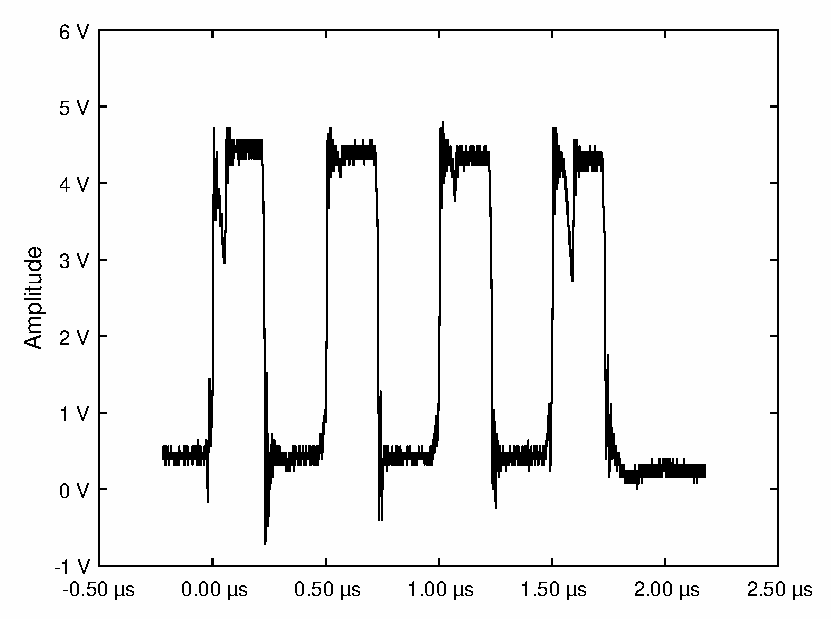
\includegraphics[width=\textwidth, trim= 0mm 0mm 0mm 0mm, clip=true]{images/tests/tx/2MHz-TX.eps}%docu
    	\caption{negatives xDSL Signal mit 2 MHz Ansteuerung}
	    \label{fig:tx2s}
	\end{subfigure}%
    \hfil %add desired spacing between images, e. g. ~, \quad, \qquad, \hfill etc.
    %(or a blank line to force the subfigure onto a new line)
    \begin{subfigure}[t]{0.31\textwidth}
    	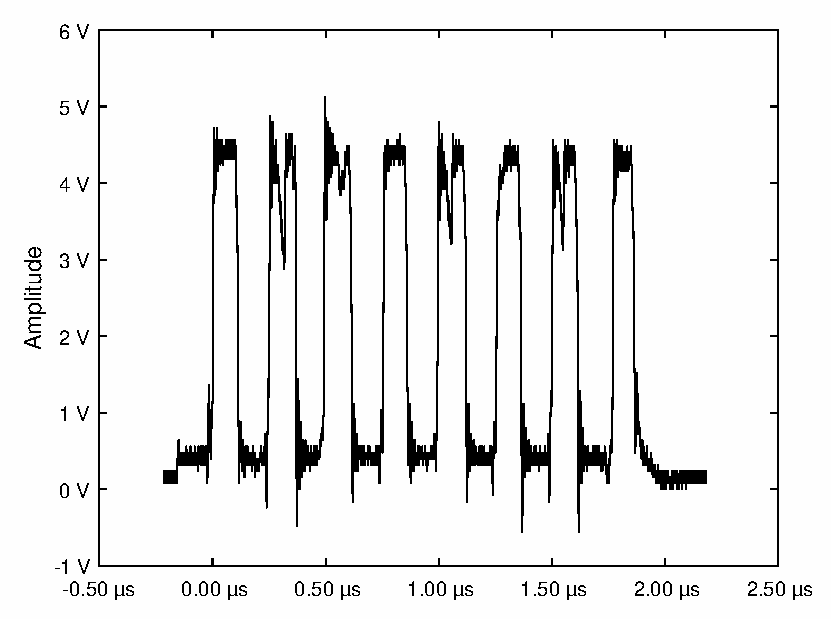
\includegraphics[width=\textwidth, trim= 0mm 0mm 0mm 0mm, clip=true]{images/tests/tx/4MHz-TX.eps}%docu
    	\caption{negatives xDSL Signal mit 4 MHz Ansteuerung}
	    \label{fig:tx4s}
    \end{subfigure}
    \hfil %add desired spacing between images, e. g. ~, \quad, \qquad, \hfill etc.
    %(or a blank line to force the subfigure onto a new line)
    \begin{subfigure}[t]{0.31\textwidth}
    	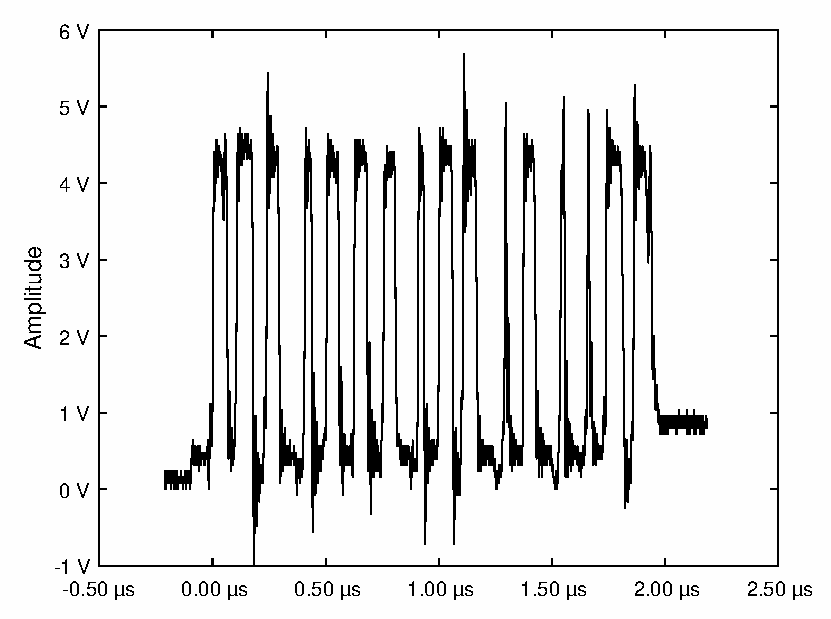
\includegraphics[width=\textwidth, trim= 0mm 0mm 0mm 0mm, clip=true]{images/tests/tx/8MHz-TX.eps}%docu
    	\caption{negatives xDSL Signal mit 8 MHz Ansteuerung}
	    \label{fig:tx8s}
    \end{subfigure}
    \hfil
    \begin{subfigure}[t]{0.31\textwidth}
    \centering
    	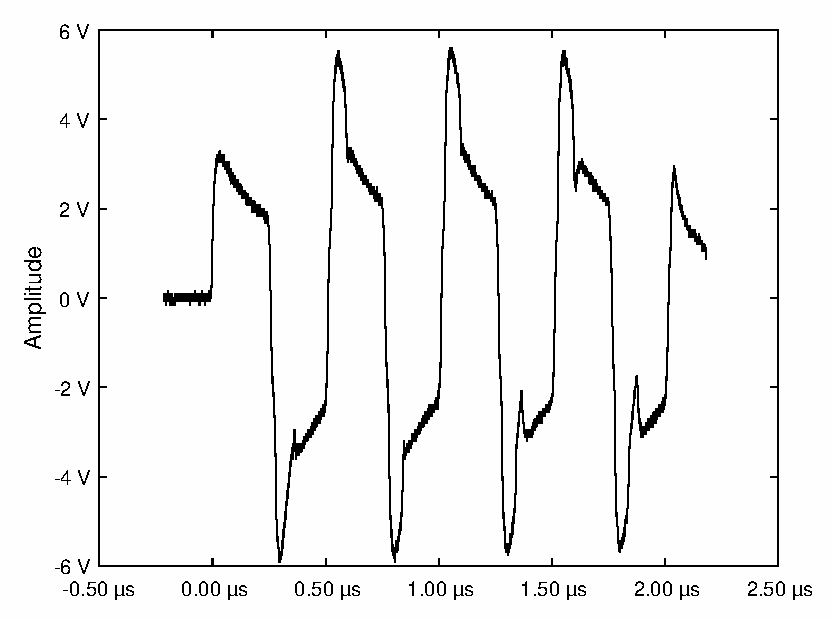
\includegraphics[width=\textwidth, trim= 0mm 0mm 0mm 0mm, clip=true]{images/tests/tx/2MHz-in.eps}%docu
    	\caption{2 MHz Burst}
	    \label{fig:tx2in}
	\end{subfigure}%
    \hfil %add desired spacing between images, e. g. ~, \quad, \qquad, \hfill etc.
    %(or a blank line to force the subfigure onto a new line)
    \begin{subfigure}[t]{0.31\textwidth}
    	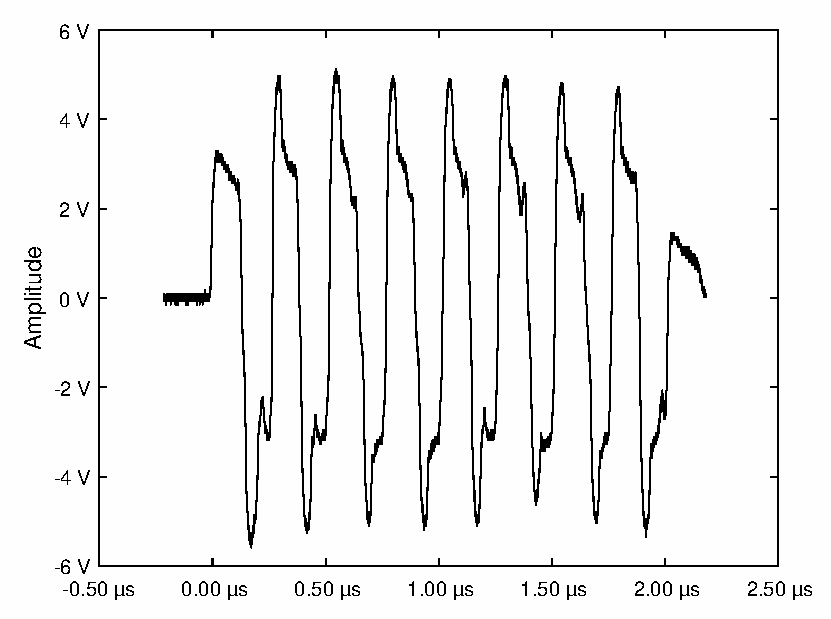
\includegraphics[width=\textwidth, trim= 0mm 0mm 0mm 0mm, clip=true]{images/tests/tx/4MHz-in.eps}%docu
    	\caption{4 MHz Burst}
	    \label{fig:tx4in}
    \end{subfigure}
    \hfil %add desired spacing between images, e. g. ~, \quad, \qquad, \hfill etc.
    %(or a blank line to force the subfigure onto a new line)
    \begin{subfigure}[t]{0.31\textwidth}
    	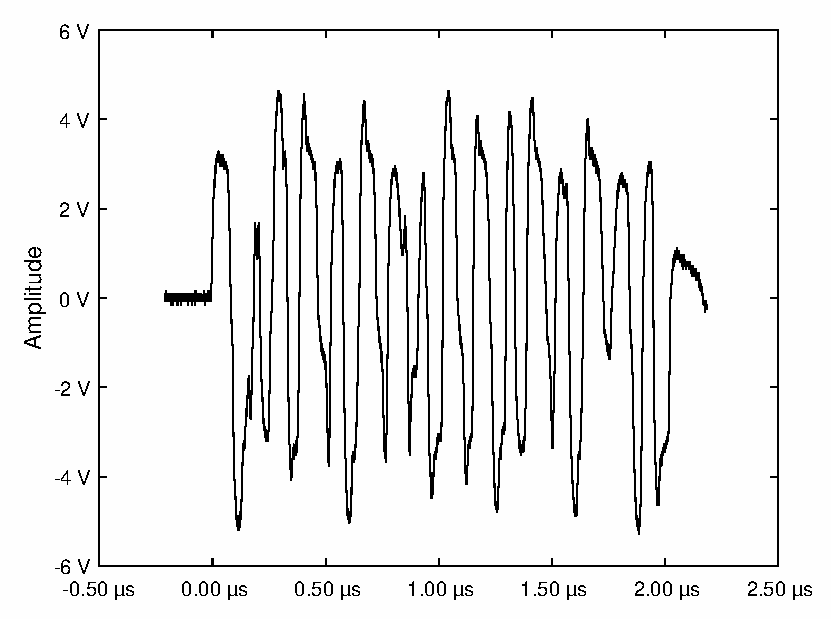
\includegraphics[width=\textwidth, trim= 0mm 0mm 0mm 0mm, clip=true]{images/tests/tx/8MHz-in.eps}%docu
    	\caption{8 MHz Burst}
	    \label{fig:tx8in}
    \end{subfigure}
	\caption{Transmitter Signale vor und nach Wandler}
	\label{fig:tx_measure}
\end{figure}\\
Da Überschwinger in den Ausgangssignalen erkennbar sind, wurde eine nachträgliche Reduzierung des Ringing-Effekts durch 100 $\Omega$ Serienwiderstände an den Eingangssignalen durchgeführt. Dies beeinflusste das Ausgangssignal des xDSL Treibers jedoch nicht. Einbrüche sind an den Ausgangssignalen in \autoref{fig:tx2s}, \autoref{fig:tx4s} und \autoref{fig:tx8s} zu erkennen, was auf eine zu große Last schließen lässt. Die Amplituden der Burst Signale nach dem Transformator brechen je nach Last ein. Zudem sehen diese nicht wie Rechtecksignale oder wie durch die Trägheit der Transformatoren gedacht wie Sinussignale aus, wie in \autoref{fig:tx2in}, \autoref{fig:tx4in} und \autoref{fig:tx8in} ersichtlich wird. Dies deutet auf eine Sättigung der Transformatoren hin, wodurch die maximale Amplitude nicht erreicht werden kann. Die Signalform wird durch die Dominanz der Induktivitäten des Bandpasses verändert, was bei der Simulation nicht berücksichtigt wurde.\\
Ohne weitere Modifikationen ist der Transmitter für die Applikation ungeeignet und sollte daher separat betrachtet werden.
\subsection{Receiver}
Der Receiver wurde als letzte Peripheriekomponente in Betrieb genommen. Dieser ist zentrales Element der Instrumentierung und muss während der Entwicklung angepasst werden, um eine bestmögliche Digitalisierung zu gewährleisten. Auch wenn die Baugruppen separat entwickelt wurden, wird nachfolgend die analoge Signalverarbeitung und die Digitalisierung zusammen betrachtet um die Testzeit zu reduzieren. Zudem zählt das Ergebnis des \ac{snr}s, welches die Genauigkeit des Receivers beschreibt.
\subsubsection*{Testaufbau und -durchführung}
Zunächst wird ein Zähler anstelle der \ac{adc}s in die Logik des \ac{cpld}s implementiert, um softwarebedingte Visualisierungsprobleme zu erkennen und zu beheben. Anschließend wird der PM5139, welcher in \autoref{sec:funktionsgen} beschrieben wird, für die Erzeugung eines Sinussignal genutzt, welches anstelle der Zählwerte visualisiert werden soll. Nachfolgend werden an diesem das Signal in Form, Amplitude und Frequenz geändert, um einen groben Überblick über das Verhalten des Receivers zu erhalten.\\
Nachdem wird zunächst der \ac{snr} bestimmt und optimiert, indem bei einer Trägerfrequenz die Amplitude soweit erhöht wird, bis der maximale Wertebereich des \ac{adc}s ($2^{14}=\pm 8191$) erreicht ist. Dabei wird das Signal über 4096 Messwerte bei 64 \ac{msps} digitalisiert und auf den \ac{pc} gespeichert, woraufhin der \ac{snr} bestimmt wird. Anschließend wird dies für diverse Verstärkungen wiederholt, um Aussagen über das Rauschen des Vorverstärkers zu treffen. Dabei wird der Widerstand $R_G$ des Vorverstärkers nach Bedarf getauscht.\\
Nachdem der \ac{snr} im Verhältnis zur Verstärkung gewählt wurde, wird die Verstärkung über den Frequenzbereich 0,5 bis 10 \ac{mhz} in 500 \ac{khz} Schritten bestimmt. Dabei wird die Amplitude des Signals soweit erhöht, bis der \ac{adc} ausgesteuert wird.
\subsubsection*{Ergebnisse}
Die Zählwerte konnten nach Anpassung der Datentypen der QT-Software visualisiert werden. Für das Sinussignal hingegen musste die Verilog Syntax genauer betrachtet werden. Dabei ergab sich, dass die geplante Biterweiterung von 14 auf 16 Bit fehlerhaft war. Dies konnte durch den Befehl $\$signed()$ kompensiert und das RF-Signal erfolgreich visualisiert werden.\\
Da der \ac{snr} nur 59,55 \ac{db} betrug, wurde der Verstärkungsfaktor über den Widerstand $R_G$ angepasst. Die Ergebnisse werden in \autoref{tab:snr_results} auf Seite \pageref{tab:snr_results} zusammengefasst. Zudem wurden die Eingänge des \ac{adc}s kurzgeschlossen und das \ac{snr} durch die maximal mögliche Auflösung ermittelt. Dabei stellte sich ein Wert von 74,45 \ac{db} heraus, welcher als mögliches Limit des \ac{adc}s zu Verfügung steht. Es wurde sich für eine Verstärkung von 13,3 dB bei einer Trägerfrequenz von 2 \ac{mhz} entschieden, da diese einen \ac{snr} 69,87 dB bieten kann. Der Widerstand $R_G$ wurde folglich auf 100 $\Omega$ erhöht, die Samplingfrequenz angepasst und der \ac{snr} bestimmt. Dabei ergab sich eine Abweichung von 0,1 \ac{db}, welche durch Messungenauigkeiten entstehen kann.
\begin{figure}[h!]
\centering
	\begin{subfigure}[t]{0.48\textwidth}
    \centering
    	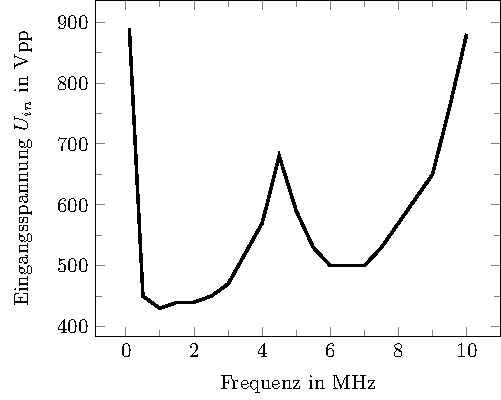
\includegraphics[width=\textwidth, trim= 0mm 0mm 0mm 0mm, clip=true]{images/tests/bandpassUin}%docu
    	\caption{benötigte Eingangsspannung des Receivers für die maximale Aussteuerung des \ac{adc}-Eingangs}
	    \label{fig:pcb_top}
	\end{subfigure}%
    \hfil %add desired spacing between images, e. g. ~, \quad, \qquad, \hfill etc.
    %(or a blank line to force the subfigure onto a new line)
    \begin{subfigure}[t]{0.48\textwidth}
    	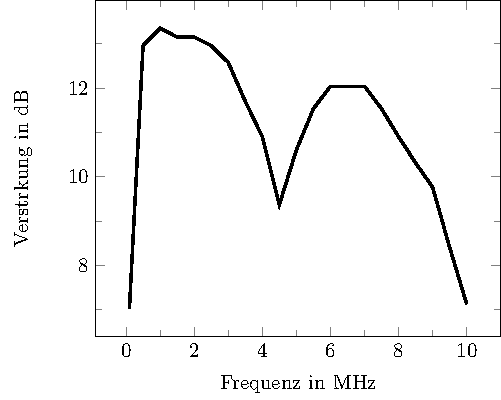
\includegraphics[width=\textwidth, trim= 0mm 0mm 0mm 0mm, clip=true]{images/tests/bandpassDB}%docu
    	\caption{Verstärkung der gesamten Receivermoduls}
	    \label{fig:pcb_bottom}
    \end{subfigure}
	\caption{Filtercharakteristik des Receivermoduls}
	\label{fig:bp_filter}
\end{figure}\\
Der Bandpass wurde nach Bestimmung des \ac{snr} erfasst, indem die Eingangsfrequenz von 0,5 \ac{mhz} bis 10 \ac{mhz} in 0,5 \ac{mhz} Schritten verändert wurde. Daraus ergaben sich die Graphen in \autoref{fig:bp_filter}. Es ist zu erkennen, dass das Filterverhalten von dem gewollten Verhalten abweicht. Jedoch verstärkt der Receiver Signale um 2 \ac{mhz} um rund 13 \ac{db}, Singale um 4 \ac{mhz} um rund 11 \ac{db} und Singale um 8 \ac{mhz} um rund 11 \ac{db}, was einen Verstärkungsfaktor von 4,4 und 3,5 entspricht.
\begin{table}[h!]
\centering
\caption{\acs{snr} in Abhängigkeit der Verstärkung und Widerstand $R_G$}
\label{tab:snr_results}
\begin{tabular}{r|>{\centering}p{2.6cm}|>{\centering}p{2.3cm}|>{\centering}p{2.3cm}|>{\centering}p{2.3cm}|c}
\textbf{$R_G$} & \textbf{Verstärkungs-faktor} & \textbf{Verstärkung} & \textbf{Eingangs-amplitude} & \textbf{Sampling-frequenz} & \textbf{\ac{snr}} \\
\cline{1-6}
8,6 $\Omega$	& 20,00 & 26,0 \ac{db} & 100 mV\ac{pp} & 64 \ac{msps} & 59,96 \ac{db} \\ 
39 $\Omega$ 	& 9,09	& 19,2 \ac{db} & 220 mV\ac{pp} & 64 \ac{msps} & 66,61 \ac{db} \\
82 $\Omega$ 	& 5,60	& 14,9 \ac{db} & 357 mV\ac{pp} & 64 \ac{msps} & 68,96 \ac{db} \\
100 $\Omega$ 	& 4,62	& 13,3 \ac{db} & 433 mV\ac{pp} & 64 \ac{msps} & 69,87 \ac{db} \\
150 $\Omega$ 	& 3,45	& 10,7 \ac{db} & 580 mV\ac{pp} & 64 \ac{msps} & 71,30 \ac{db} \\
220 $\Omega$ 	& 2,06	& 6,3  \ac{db} & 970 mV\ac{pp} & 64 \ac{msps} & 71,86 \ac{db}
\end{tabular}
\end{table}
\subsection{Signalintegrität und Kopplungen}
Um die induktive Entkopplung der analogen Komponenten und somit die Stabilität der Spannungsversorgung im Betrieb sicherzustellen muss dieser Test durchgeführt werden. Gleichzeit kann mit diesem das Nachschwingverhalten von digitalen Signalen überprüft werden. Das Ringing stellte eine zusätzlich Belastung der Spannungsversorgung dar und führt zur Entstehung von Störsignalen, welche abgestrahlt werden können. Daher werden diese detektiert um eine Optimierung der Instrumentierung zu ermöglichen.
\subsubsection*{Testaufbau und -durchführung}
Zunächst wird mit dem Oszilloskop HMO3524 die Welligkeit aller Spannungsversorgungen im Betrieb gemessen und untersucht. Dabei kann das Spektrum untersucht werden um Rückschlüsse auf die Störquellen zu erhalten. Wenn Frequenzen um 64 \ac{mhz} oder einem vielfachen davon im Spektrum sichtbar sind, wird eine Nahfeldsonde benötigt, um Rückschlüsse über den Entstehungsort zu erhalten. Zudem kann eine Strommesszange in Verbindung mit einen Spektrum-Analysator verwendet werden, um Frequenzen auf der Zuleitung und dem Anschluss zur Sonde zu erkennen. Dabei wird ein \ac{usb} Kabel durch die Strommesszange geführt und das Spektrum visualisiert.
\subsubsection*{Ergebnisse}
Die \ac{fft} Funktion des Oszilloskop HMO3524 zeigte einen deutlichen Anstieg des 64 \ac{mhz} Signals und der zweiten Oberwelle bei 192 \ac{mhz}. Daher wurde eine Nafeldsonde an den Testpunkten wie in der \autoref{fig:measurepoints} positioniert und das Spektrum von einen bis 640 \ac{mhz} mit dem Spectrum Analyzer FSL3 aus \autoref{sec:analyzer} aufgenommen. Die Ergebnisse sind in \autoref{fig:signal_int} aufgeführt.
\begin{figure}[h!]
	\centering
	\begin{subfigure}[t]{0.42\textwidth}
    \centering
\begin{annotatedFigure}
	{\includegraphics[page=4,width=1\textwidth, trim= 0mm 0mm 0mm 0mm, clip=true]{images/pcb/Job2.PDF}}
	\draw[line width=1.0mm] (0.2838,0.048) -- (0.3324,0.048) node[fill=black,thick,shape=circle,inner sep=2pt,font=\sffamily,text=white] {a};
	\draw[line width=1.0mm] (0.1627,0.082) -- (0.2101,0.044) node[fill=black,thick,shape=circle,inner sep=2pt,font=\sffamily,text=white] {b};
	\draw[line width=1.0mm] (0.3721,0.162) -- (0.4214,0.1974) node[fill=black,thick,shape=circle,inner sep=2pt,font=\sffamily,text=white] {c};
	\draw[line width=1.0mm] (0.1655,0.458) -- (0.1655,0.406) node[fill=black,thick,shape=circle,inner sep=2pt,font=\sffamily,text=white] {d};
	\draw[line width=1.0mm] (0.0543,0.486) -- (0.0543,0.432) node[fill=black,thick,shape=circle,inner sep=2pt,font=\sffamily,text=white] {e};
	\draw[line width=1.0mm] (-0.0037,0.404) -- (0.0543,0.404) node[fill=black,thick,shape=circle,inner sep=2pt,font=\sffamily,text=white] {f};
	\draw[line width=1.0mm] (0.4125,0.534) -- (0.4742,0.534) node[fill=black,thick,shape=circle,inner sep=2pt,font=\sffamily,text=white] {g};
	\draw[line width=1.0mm] (0.2345,0.466) -- (0.2962,0.466) node[fill=black,thick,shape=circle,inner sep=2pt,font=\sffamily,text=white] {h};
	\draw[line width=1.0mm] (0.122,0.217) -- (0.122,0.174) node[fill=black,thick,shape=circle,inner sep=2pt,font=\sffamily,text=white] {i};
	\draw[line width=1.0mm] (0.122,0.221) -- (0.122,0.274) node[fill=black,thick,shape=circle,inner sep=2pt,font=\sffamily,text=white] {j};
	\draw[line width=1.0mm] (0.1889,0.124) -- (0.1306,0.124) node[fill=black,thick,shape=circle,inner sep=2pt,font=\sffamily,text=white] {k};
	\draw[line width=1.0mm] (0.2099,0.124) -- (0.2099,0.092) node[fill=black,thick,shape=circle,inner sep=2pt,font=\sffamily,text=white] {l};
	\draw[line width=1.0mm] (0.1789,0.144) -- (0.2406,0.144) node[fill=black,thick,shape=circle,inner sep=2pt,font=\sffamily,text=white] {m};
	\draw[line width=1.0mm] (0.2862,0.144) -- (0.3434,0.144) node[fill=black,thick,shape=circle,inner sep=2pt,font=\sffamily,text=white] {n};
	\draw[line width=1.0mm] (0.1705,0.2456) -- (0.2122,0.2236) node[fill=black,thick,shape=circle,inner sep=2pt,font=\sffamily,text=white] {o};
\end{annotatedFigure}
    \caption{Ground Plane und Komponenten auf der Platinenoberseite - Richtung der Nahfeldsonde}
    \label{fig:system_layout}
    \end{subfigure}%
    \hfil
    \begin{subfigure}[t]{0.42\textwidth}
    \centering
    \begin{annotatedFigure}
	{\includegraphics[page=5,width=1\textwidth, trim= 0mm 0mm 0mm 0mm, clip=true]{images/pcb/Job2.PDF}}
	\draw[line width=1.0mm] (0.1505,0.2456) -- (0.1922,0.2236) node[fill=black,thick,shape=circle,inner sep=2pt,font=\sffamily,text=white] {p};
	\draw[line width=1.0mm] (0.5074,0.206) -- (0.4768,0.178) node[fill=black,thick,shape=circle,inner sep=2pt,font=\sffamily,text=white] {q};
	\draw[line width=1.0mm] (0.226,0.1296) -- (0.276,0.1296) node[fill=black,thick,shape=circle,inner sep=2pt,font=\sffamily,text=white] {r};

	\draw[line width=1.0mm] (0.2037,0.534) -- (0.256,0.534) node[fill=black,thick,shape=circle,inner sep=2pt,font=\sffamily,text=white] {s};
\end{annotatedFigure}
	\caption{Power Plane und Komponenten auf Platinenunterseite - Richtung der Nahfeldsonde}
    \end{subfigure}
    \caption{Messpunkte der Nahfeldsonde für die Signalintegrität in \autoref{sec:signal_db}}
    \label{fig:measurepoints}
\end{figure}\\
Nach Betrachtung der Ergebnisse ergab sich, dass die Oberwellen eine höhere Amplitude als das 64 \ac{mhz} Signal aufweisen. Daher wird vermutet, dass das Filter zwar wirkt, jedoch durch eine schlechte Impedanz an Wirkung verliert. Die Vermutung wurde durch eine Spektralanalyse mit einer Strommesszange an dem nicht geschirmten \ac{usb} Kabel bestätigt, da 64 \ac{mhz} und dessen Oberwellen auf der Versorgungsleitung erkennbar sind (\autoref{fig:strom_spannung}). Weiterhin wurde die Signalleitung zur Sonde (\autoref{fig:strom_sonde}) mit der Strommesszange gemessen und das Spektrum wies die gleichen Amplituden auf. Dies lässt den eindeutig Schluss zu, dass ein Ground-bouncing vorherrscht. Somit wurde die Anordnung der Bypass-Kondensatoren des \ac{adc}s näher betrachtet. Der Abstand zwischen dem digitalen Versorgungspin und dem Bypass beträgt rund 2 mm, wischen den analogen Versorgungspins und den Bypass Kondensatoren 3 und 4,4 mm. Die Faustformel besagt, dass 1 mm Leiterbahnweg einen 1 nH entspricht. Somit ergibt sich die \autoref{tab:imp_caps}. Die Traget-Impedanz sollte bei 0,01 $\Omega$ liegen, damit die Filtercharakteristik auch bei den Oberwellen bis 6,4 \ac{ghz} wirken kann.
\newcolumntype{L}[1]{>{\RaggedRight\hspace{0pt}}p{#1}}
\newcolumntype{R}[1]{>{\RaggedLeft\hspace{0pt}}p{#1}}
\begin{table}[h!]
\centering
\caption{Impedanz in Abhängigkeit von der Frequenz und dem Abstand}
\label{tab:imp_caps}
\begin{tabular}{r|R{2,4cm}|R{2,4cm}|R{2,4cm}|R{2,4cm}}
\textbf{Frequenz} & \textbf{Impedanz bei 0,2 mm} & \textbf{Impedanz bei 2 mm} & \textbf{Impedanz bei 3 mm} & \textbf{Impedanz bei 4,4 mm}\\
\cline{1-5}
64 \ac{mhz} & 0,08 $\Omega$ & 0,8 $\Omega$ & 1,2  $\Omega$ & 1,77  $\Omega$ \\
128 \ac{mhz} & 0,16 $\Omega$ & 1,6 $\Omega$ & 2,41  $\Omega$ & 3,54  $\Omega$ \\
192 \ac{mhz} & 0,24 $\Omega$ & 2,41 $\Omega$ & 3,62  $\Omega$ & 5,31  $\Omega$ \\
256 \ac{mhz} & 0,32 $\Omega$ & 3,21 $\Omega$ & 4,83  $\Omega$ & 7,07  $\Omega$ \\
320 \ac{mhz} & 0,40 $\Omega$ & 4,02 $\Omega$ & 6,03  $\Omega$ & 8,85  $\Omega$ \\
512 \ac{mhz} & 0,64 $\Omega$ & 6,43 $\Omega$ & 9,65 $\Omega$ & 14,15  $\Omega$ \\
1024 \ac{mhz} & 1,28 $\Omega$ & 12,86 $\Omega$ & 19,30 $\Omega$ & 28,31  $\Omega$
\end{tabular}
\end{table}\\
Aus \autoref{tab:imp_caps} ist ersichtlich, dass die Traget-Impedanz von 0,01 $\Omega$ nicht erreicht wurde. Daher ist eine Kompensation des Ground-bouncing Effekts ohne ein Redesign nicht realisierbar.
\subsection{Demodulierung}\label{sec:demodulation_results}
Aus Zeitgründen konnte die Logik der Demodulierung nicht mit der aktuellen Hardware getestet werden. Jedoch wurde diese in der Bachelor Thesis von Herrn A. Rehn 2014 deklariert und ausführlich getestet, wodurch diese nachträglich implementiert werden muss.
\clearpage
\section{Integrationstest}\label{sec:inttest}%(Integration-Test)
\begin{figure}[h!]
\centering
	\begin{subfigure}[b]{0.499\textwidth}
    \centering
    	\includegraphics[page=3,width=\textwidth, trim= 65mm 5mm 65mm 0mm, clip=true]{images/pcb/Job2.PDF}%docu
    	\caption{Oberseite der Dopplerinstrumentierung}
	    \label{fig:pcb_top}
	\end{subfigure}%
    \hfil %add desired spacing between images, e. g. ~, \quad, \qquad, \hfill etc.
    %(or a blank line to force the subfigure onto a new line)
    \begin{subfigure}[b]{0.499\textwidth}
    	\includegraphics[page=2, width=\textwidth, trim= 65mm 5mm 65mm 0mm, clip=true]{images/pcb/Job2.PDF}%docu
    	\caption{Unterseite der Dopplerinstrumentierung}
	    \label{fig:pcb_bottom}
    \end{subfigure}
    \hfil
    ~
    \begin{subfigure}[b]{1\textwidth}
    	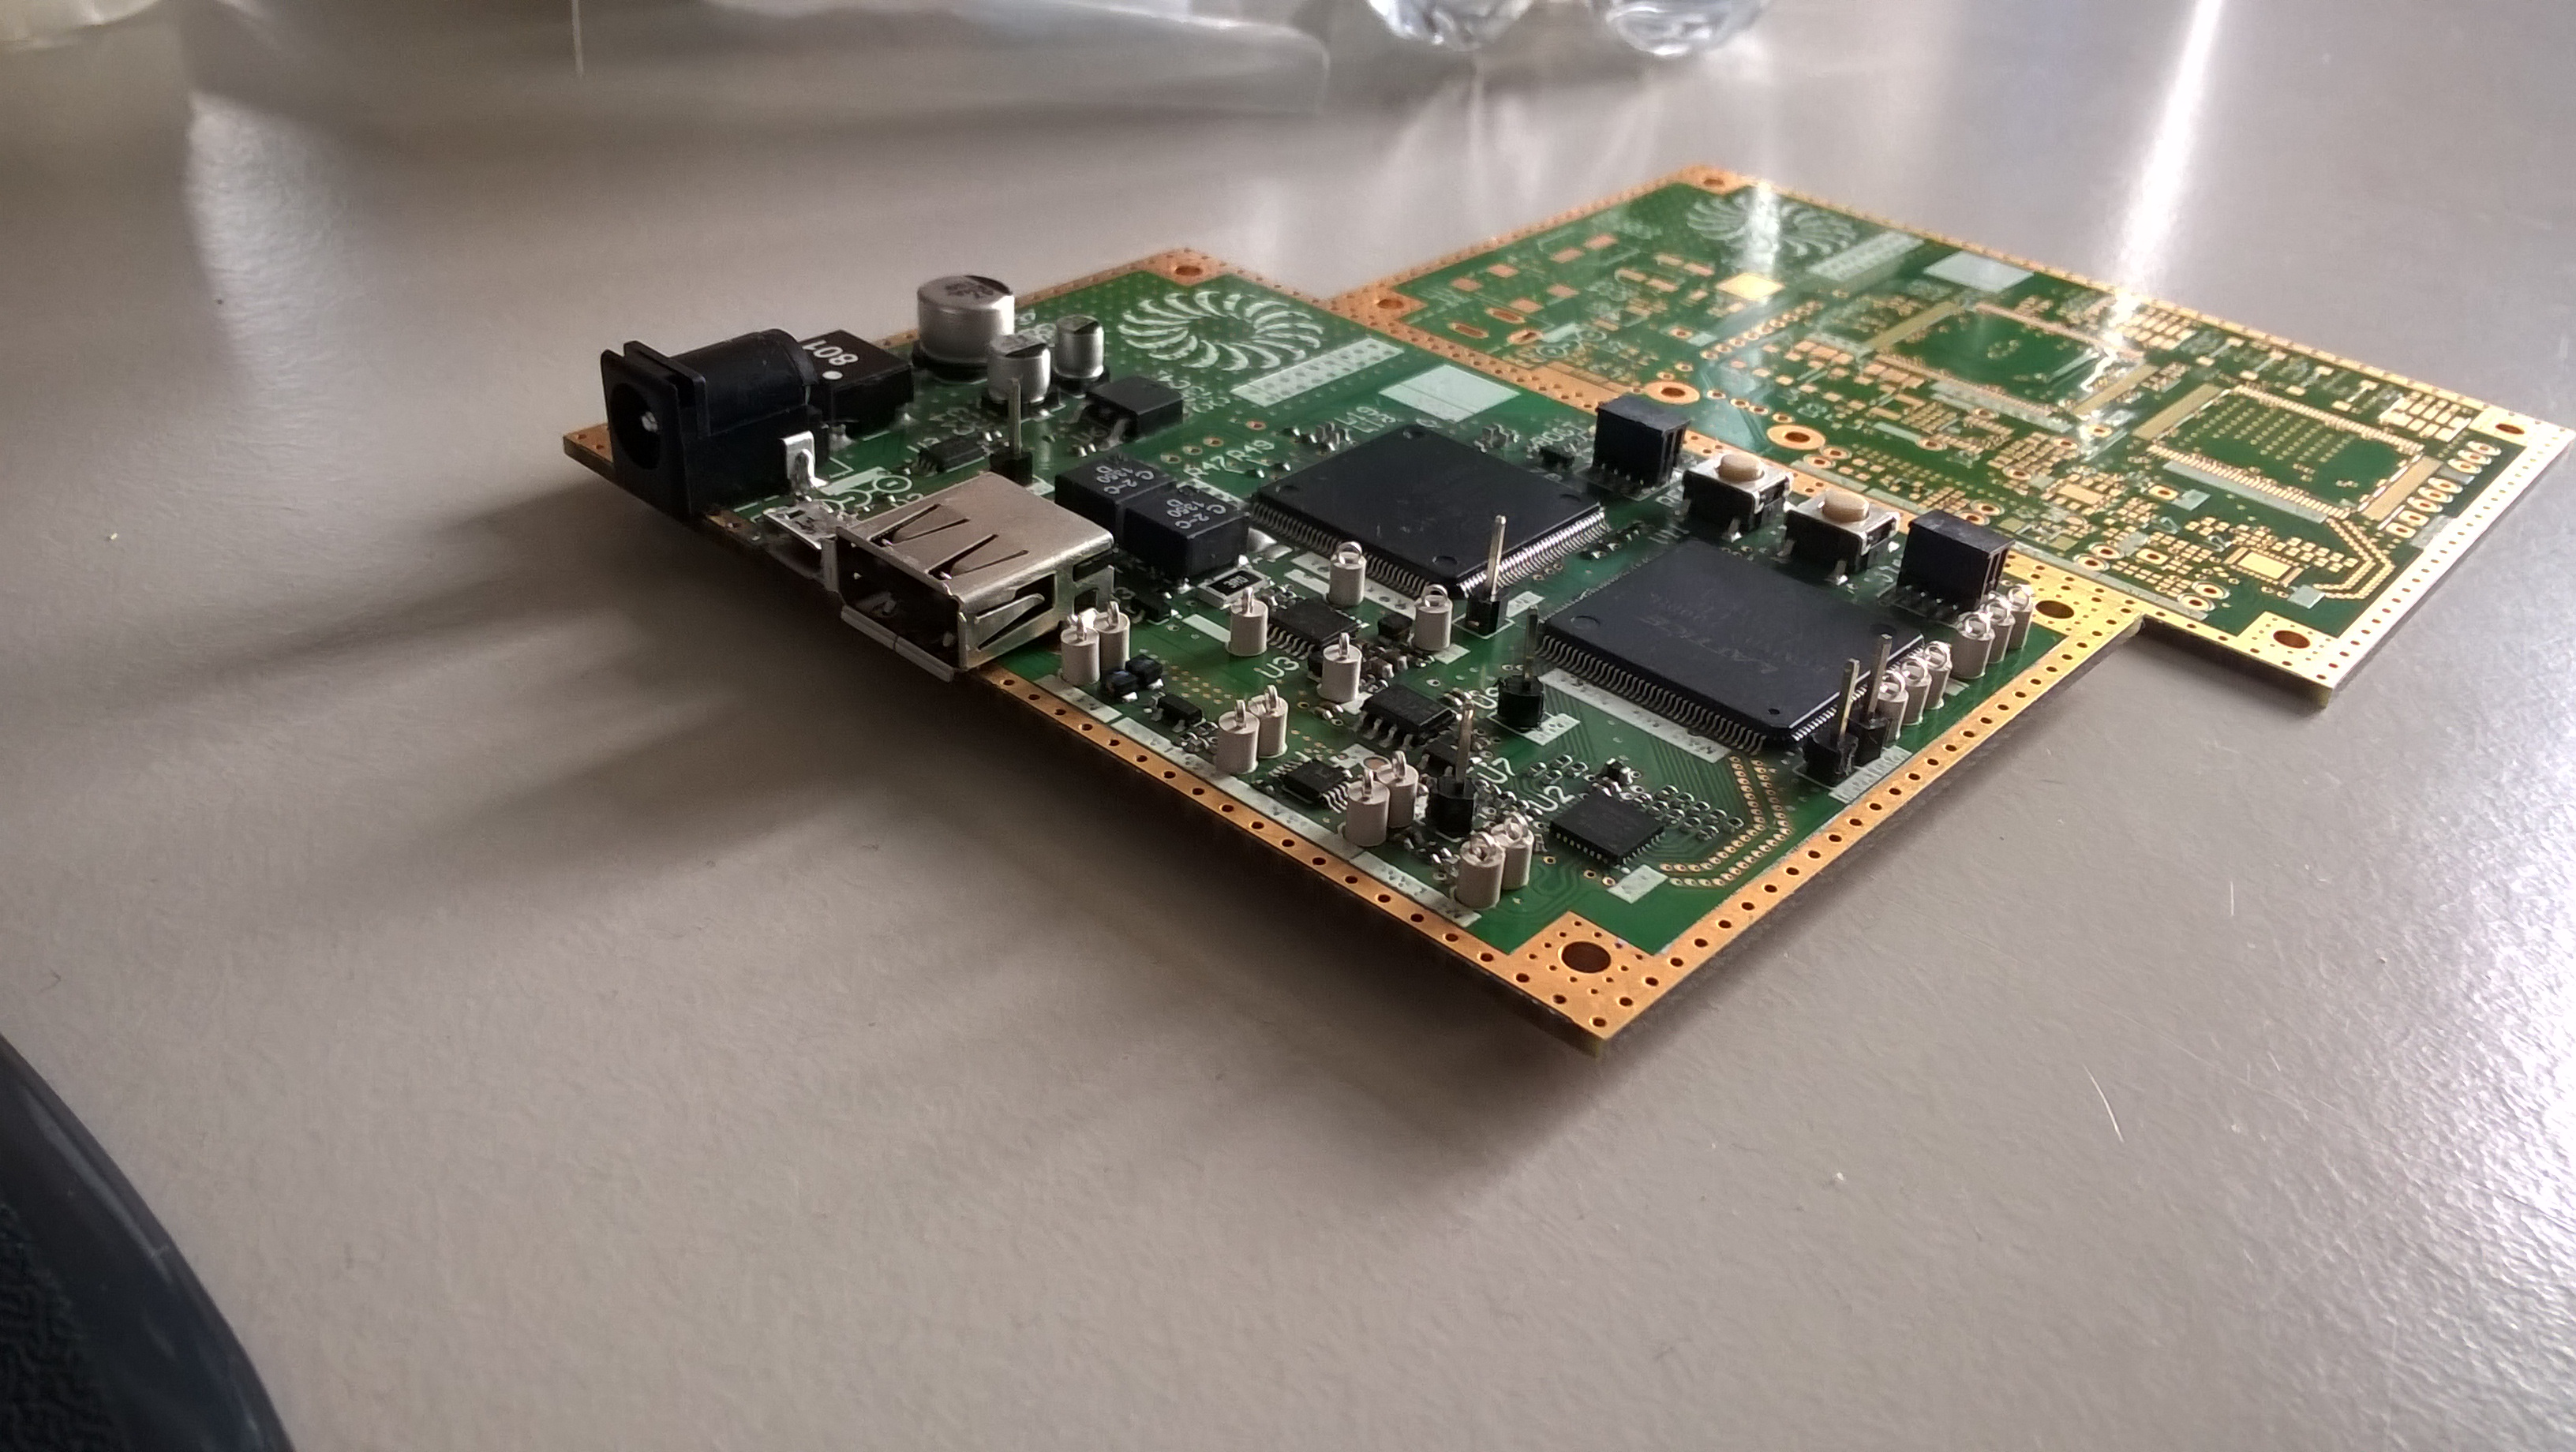
\includegraphics[width=\textwidth, trim= 230mm 155mm 0mm 65mm, clip=true]{images/pcb/WP_20150709_002}
    	\caption{\ac{pcb} der Dopplerinstrumentierung (vorne bestückt, hinten nicht bestückt)}
		\label{fig:3Dpcb}
    \end{subfigure}
	\caption{Ergebniss des \acs{pcb}-Layouts}\label{fig:pcb}
\end{figure}
Nachdem die grundlegenden Funktionalitäten verifiziert wurden, konnte das System in Betrieb genommen werden. Wie in \autoref{sec:demodulation_results} beschrieben erfolgt keine Demodulierung des RF-Signals. Hingegen werden 14-Bit RF-Signale durch die geschriebene QT-Software erfolgreich dargestellt. Die OnTheFly Änderung von Parametern über die QT-Software funktioniert nur bei der Starttiefe der \ac{roi}. Dies deutet auf ein Problem der Logik des \ac{cpld}s hin, da der \ac{spi} Datentransfer wie erwartet arbeitet und aktuell alle Parameter transferiert werden.\\
Durch die mangelnde Funktionalität des Transmitters, konnte kein Transducer erfolgreich in Betrieb genommen werden. Jedoch können die Signale des Transmitters durch den Receiver digitalisiert und mit der QT-Software dargestellt werden.\\
Durch die verspätete Lieferung des Gehäuses konnten keine Aussparungen für das Frontblech des Gehäuses durchgeführt werden. Dies beeinträchtigt die Funktionalität der Applikation jedoch nicht, wodurch dies nachträglich durchgeführt werden kann. Zudem sind die vorgesehen Montagelöcher für gängige Schrauben und Abstandshalter zu klein, wodurch eine Montage erschwert wird.\\
Das realisierte System läuft grundsätzlich über einen Testzeitraum von 10 Minuten stabil. Dabei treten Darstellungsfehler auf, welche auf ein fehlendes Byte während eines Frames hindeuten. Dies wird ersichtlich, wenn das \ac{fifo} des \ac{cpld}s nicht genügend Samples zu Verfügung stellen kann. Durch das fehlende Byte wird der 16-Bit Wert geshiftet, was einen Offset und ein Skalierungsproblem zur Folge hat.\\
Eine Synchronisierung wischen \ac{pc} und LPC4337 wurde nicht realisiert, da der Fokus auf der Umsetzung der grundlegenden Funktion lag. Daher benötigt der Test-\ac{pc} 18,8 MB Arbeitspeicher und rund 23 bis 48 \% der Intel I5 Rechenleistung.
\chapter{Diskussion und Ausblick}
In diesem Kapitel wird das Erreichte zunächst in \autoref{sec:discussion_results} zusammengefasst. Aufkommende Fragen während der Testdurchführung und der Testergebnisse werden anschließend in \autoref{sec:discussion_testresults} analysiert und ein Fazit durch Schlussfolgerungen dargestellt. Weiterhin wird die Realisierung der Anforderungen in \autoref{sec:discuss_all} und deren Umsetzung in \autoref{sec:discuss_tasks} analysiert und objektiv bewertet. Abgeschlossen wird das Kapitel, indem in \autoref{sec:futurework} Verbesserungspotentiale aufgezeigt und mögliche Weiterentwicklungen des Systems und dessen Module erbracht werden.
\section{Zusammenfassung der Ergebnisse}\label{sec:discussion_results}
Im Rahmen der vorliegenden Arbeit wurde eine Dopplerinstrumentierung entwickelt, welche das Messen von Ultraschall Dopplerschiebefrequenzen bedingt erlaubt. Die aus dem Messverfahren resultierenden M-Mode und Doppler Spektrogramm Darstellungen zu realisieren gelang in den zur Verfügung stehenden Zeitraum nicht. Dafür konnten die grundlegenden Funktionen für die Realisierung des Messverfahrens, sowie der Visualisierung umgesetzt werden. Eine Echtzeitvisualisierung der RF-Daten konnte erfolgreich auf dem \ac{pc} dargestellt werden, was die Grundlage für die Visualisierung der Graphen bildet und die Möglichkeiten des Systems zeigt. Durch die Nutzung eines Embedded Systems kann die analoge durch eine digitale Demodulierung ersetzt werden, was nicht nur kosteneffizienter ist, sondern mehr Informationen pro Hardware Channel und Digitalisierung bietet. Die entwickelte Instrumentierung    kann somit als Alternative für die Erkennung von Embolien dienen, wenn die erkannten Probleme behoben und die Software komplettiert ist.
\section{Diskussion der Testergebnisse und der Testdurchführung}\label{sec:discussion_testresults}
\subsubsection*{Transmitter}
Der Transmitter erfüllt die Anforderungen nicht, da er die zu nutzenden Frequenzen nicht konstant und 8 \ac{mhz} gar nicht treiben kann. Die Hardware weicht soweit von der Simulation ab, dass es in der zu Verfügung stehenden Zeit unmöglich war, einen plausiblen Grund für das Versagen des xDSL Treibers zu finden. Aus wirtschaftlichen und zeitlich Gründen sollten daher Alternativen bevorzugt werden. Weiterhin muss der Transmitter während der Brustphase von dem Receiver entkoppelt werden, da die Induktivitäten des Bandpassfilters die zu sendende Signalform beeinflussen. Dies könnte \ac{zb} durch einen SPDT Schalter erfolgen.
\section{Diskussion zur Einhaltung aller Anforderungen}\label{sec:discuss_all}
\subsubsection*{Software- und Hardwareanforderungen}
Die Anforderungen an die Energieversorgung sind nach einer Anpassung der ersten Spannungsreduzierung erfolgreich umgesetzt wurden. Der integrierte Verpolschutz schützt das System erfolgreich bei verpolten Eingängen und sollte beibehalten werden. Die genierten Spannungen unterliegen keinen Einbrüchen. Der Abstand der Bypasskondensatoren zu den \ac{ic}s ist zu groß für die bei dieser Applikation vorkommenden Frequenzen und deren Oberwellen. Somit ist das Filterverhalten und die induktive Entkopplung nur bei geringeren Frequenzen gewährleistet. Dies macht sich durch Brummspannung von $\pm$ 5 bis 10 mV der Spannung bemerkbar, wodurch das \ac{snr} reduziert wird. Es ist davon auszugehen, dass ein Ground-bouncing mit der Taktfrequenz des \ac{adc} \ac{ic}s verursacht wird, da das Filterverhalten mangelhaft ist. Eine Kompensation des Problems kann dabei den möglichen \ac{snr} erhöhen wodurch Amplituden im $\mu$V Bereich unterschieden werden können. Die Software- und Hardwareanforderungen wurden teilweise realisiert. Dabei konnten die \ac{emi} Richtlinien durch das vorkommende Nachschwingverhalten der Spannungsversorgung nicht eingehalten werden und eine Visualisierung des aktuell angeschlossenen Transducers nicht realisiert. 
\subsubsection*{Systemanforderungen}
Das Netzteil GXM60-19A04 ist nach EN60601 zugelassen, wodurch dieses in medizinischen Bereichen genutzt werden kann. Weiterhin besitzt die Platine einen NXP LPC4337, welcher als Kern einen asymmetrischen ARM\SymbReg Cortex\SymbReg-M4/M0 besitzt und ausreichend Reserven für nachträgliche Implementierungen bietet. Die \ac{usb}-micro Buchse wurde vorgesehen, ist jedoch durch einen Layoutfehler nicht nutzbar und wurde durch eine direkte Anbindung eines \ac{usb}-Kabels ersetzt. Bei der Montage der \ac{usb}-micro Buchse muss beanstandet werden, dass diese sehr schwer zu positionieren ist. Ein alternatives Package der Buchse könnte die Montage drastisch vereinfachen.
\subsubsection*{Benutzeranforderungen}
Eine Umsetzung der Benutzeranforderungen erfolgte zielstrebig. Das System besteht aus einer Platine, welche über eine QT-Software angesteuert wird. Dabei ist die QT-Plattform unter Linux Distributionen und Microsoft\SymbC Windows\SymbReg lauffähig. Jedoch können durch die verringerte Funktionsfähigkeit des Transmitters keine Transducer im Frequenzbereich von 2, 4 und 8 \ac{mhz} betrieben werden. Außerdem konnte durch Zeitmangel keine Demodulierung implementiert werden, wodurch keine I/Q-, sondern RF-Werte übertragen werden. Die implementierten Schnittstellen erlauben 96 I/Q-Werte pro \ac{prf} zu übertragen, wodurch die Anforderung der Datenübertragung teilweise realisiert werden konnte.

\section{Diskussion der Ergebnisse bzgl. der Aufgabenstellung}\label{sec:discuss_tasks}
Durch die Nutzung neuer \ac{ic}s, welche für weitere Entwicklungen Reserven bieten müssen, verlagerte sich der Schwerpunkt der Arbeit von der Applikation hin zur Hardware und deren Inbetriebnahme. Aus diesem Grund bietet diese Arbeit keinen implementierten Algorithmus zur eindeutigen Emboliedetektion und spricht diese Thematik nicht an. Mit der Inbetriebnahme der neuen \acs{ic}s und deren Logik, welche die realisierte Software und Schnittstellen beinhaltet, wurde der Grundstein für eine möglichst detailliere Emboliedetektion gelegt, indem die Möglichkeiten des Systems in dieser Arbeit dargestellt sind. Eine Ansteuerung der Transducer konnte durch die mangelhafte Transmitterschaltung nicht realisiert werden, wodurch keine Erfassung von Ultraschallsignalen möglich ist. Die Datenrate für die Übertragung der I/Q-Signale konnte drastisch erhöht und eine \ac{gui}-Implementierung ohne M-Mode und Spektrogramm Algorithmen erarbeitet werden.\\
Das entwickelte System kann als Grundlage für die Weiterentwicklung der Applikation verwendet werden, wenn die Erkenntnisse der Arbeit umgesetzt werden.
\section{Verbesserungspotentiale und Ausblick}\label{sec:futurework}
\subsubsection{Spannungsversorgung}

\subsubsection{Receiver}
\subsubsection{Steuerung und Demodulierung}
\subsubsection{Kommunikation und Datenübertragung}
\subsubsection{Visualisierung}
%
%
%

\subsubsection{Layout und Hardware}
\subsubsection{Logik und Software}

\subsubsection{Kostenreduzierung}
Da im Rahmen dieser Arbeit eine Basis für eine Dopplerinstrumentierung entwickelt wurde, und die nötigten Implementierungen der Hard- und Software schwer Abzuschätzen waren, wurde sich für das größte \ac{cpld} und einen der größten asymmetrischen ARM\SymbReg Cortex\SymbReg-M4/M0 \ac{mcu}s entschieden. Diese können nach Bedarf durch kleinere Chips ersetzt werden. So stehen \ac{zb} für den NXP LPC4337 pinkompatible Alternativen mit ARM\SymbReg Cortex\SymbReg-M3 Kern (LPC1800 Serie) oder kleinere (LPC4300 Serie) zu Verfügung. Die \ac{lut} Anzahl des \ac{cpld}s hingen ist pinabhängig, wodurch ein Redesign nötig ist. 

\chapter*{Schlusswort}
\addcontentsline{toc}{chapter}{Schlusswort}
Ich möchte mich bei allen bedanken, die zu dieser Arbeit beigetragen haben. Besonders möchte ich mich bei meinen betreuenden Professor Herr \gutachterA \ für die Betreuung und die Überlassung des Themas bedanken. Zudem Herrn \gutachterB, welcher mir selbstlos in den Themengebieten \ac{emi} und Signalintegrität zur Seite stand. Des weiteren Herrn Dr.-Ing. Gert Schönfelder für Inspirationen zur Realisierung der Hardware, sowie {\href{mailto:schilling@hs-ulm.de}{Herrn Schilling-Kästle} für die schnelle Umsetzung des \ac{pcb} Layouts, der Bestellung der \ac{bom} und seiner beispiellosen Unterstützung. Hiermit möchte ich mich auch bei meinen Eltern, meiner Schwester und meiner Freundin Nadine für Ihre Unterstützung sowie das Korrekturlesen der Arbeit bedanken.


%\phantomsection
\addcontentsline{toc}{chapter}{Literaturverzeichnis}
\bibliographystyle{IEEEtran}
\bibliography{literatur}
\appendix
%\begin{landscape}
\chapter{Testergebnisse}
\section{\ac{snr}}
%\lstinputlisting[caption=Matlab \ac{snr} Test Skript, escapechar=, label=lst:matlab_snr, style=Matlab]{sourcecode/Test_SNR.m}
\begin{figure}[ht!]
	\centering
	\begin{subfigure}[t!]{0.82\textwidth}
		\centering
  		\includegraphics[page=1,width=\textwidth, trim= 31mm 178mm 36mm 22mm, clip=true]{attachment/Impedanzen_Sonden.pdf}% \\[.5cm]
 		\caption{Gel + Hand}
 		\label{fig:2_sig}
  	\end{subfigure}
  	\begin{subfigure}[t!]{0.82\textwidth}
	  	\centering
  		\includegraphics[page=1,width=\textwidth, trim= 26mm 40mm 36mm 160mm, clip=true]{attachment/Impedanzen_Sonden.pdf} %\\[.5cm]
  		\caption{Luft}
 		\label{fig:snr_2_script}
  	\end{subfigure}
  	\caption{2 \ac{mhz} Feroperm Kupferhülse + Uhu-tinse (page 1)}
\end{figure}
\clearpage

\begin{figure}[ht!]
	\centering
	\begin{subfigure}[t!]{0.82\textwidth}
	  	\centering
  		\includegraphics[page=3,width=\textwidth, trim= 27mm 63mm 37mm 137mm, clip=true]{attachment/Impedanzen_Sonden.pdf} %\\[.5cm]
  		\caption{normal page 3}
 		\label{fig:snr_2_script}
  	\end{subfigure}
  	\begin{subfigure}[t!]{0.82\textwidth}
	  	\centering
  		\includegraphics[page=5,width=\textwidth, trim= 26mm 64mm 37mm 137mm, clip=true]{attachment/Impedanzen_Sonden.pdf} %\\[.5cm]
  		\caption{im Kupferring page 5}
 		\label{fig:snr_2_script}
  	\end{subfigure}
  	\caption{2 \ac{mhz} Kristall (Luft) }
\end{figure}
\clearpage

\begin{figure}[ht!]
	\centering
	\begin{subfigure}[t!]{0.82\textwidth}
	  	\centering
  		\includegraphics[page=6,width=\textwidth, trim= 28mm 178mm 39mm 22mm, clip=true]{attachment/Impedanzen_Sonden.pdf} %\\[.5cm]
  		\caption{Gel + Hand}
 		\label{fig:snr_2_script}
  	\end{subfigure}
  	\begin{subfigure}[t!]{0.82\textwidth}
	  	\centering
  		\includegraphics[page=6,width=\textwidth, trim= 32mm 42mm 39mm 158mm, clip=true]{attachment/Impedanzen_Sonden.pdf} %\\[.5cm]
  		\caption{in Luft}
 		\label{fig:snr_2_script}
  	\end{subfigure}
  	\caption{2,25 \ac{mhz} Feroperm in Kupferhülse + Uhu-tinse (page 6)}
\end{figure}
\clearpage

\begin{figure}[ht!]
	\centering
	\begin{subfigure}[t!]{0.82\textwidth}
	  	\centering
  		\includegraphics[page=8,width=\textwidth, trim= 26mm 170mm 47mm 30mm, clip=true]{attachment/Impedanzen_Sonden.pdf} %\\[.5cm]
  		\caption{schwarz}
 		\label{fig:snr_2_script}
  	\end{subfigure}
  	\begin{subfigure}[t!]{0.82\textwidth}
	  	\centering
  		\includegraphics[page=8,width=\textwidth, trim= 38mm 55mm 47mm 144mm, clip=true]{attachment/Impedanzen_Sonden.pdf} %\\[.5cm]
  		\caption{weiß}
 		\label{fig:snr_2_script}
  	\end{subfigure}
  	\caption{4 \ac{mhz} Sonde (Hollerith?) (page 8)}
\end{figure}
\clearpage


\begin{figure}[ht!]
	\centering
	\begin{subfigure}[t!]{0.82\textwidth}
	  	\centering
  		\includegraphics[page=10,width=\textwidth, trim= 39mm 64mm 47mm 136mm, clip=true]{attachment/Impedanzen_Sonden.pdf} %\\[.5cm]
  		\caption{schwarz}
 		\label{fig:snr_2_script}
  	\end{subfigure}
  	\begin{subfigure}[t!]{0.82\textwidth}
	  	\centering
  		\includegraphics[page=10,width=\textwidth, trim= 39mm 178mm 47mm 22mm, clip=true]{attachment/Impedanzen_Sonden.pdf} %\\[.5cm]
  		\caption{weiß}
 		\label{fig:snr_2_script}
  	\end{subfigure}
  	\caption{8 \ac{mhz} Sonde (Hollerith?) (page 10)}
\end{figure}
\clearpage
%\end{landscape}

\chapter{Dokumente}
\begin{center}
\begin{tabular}{|p{12cm}|c|}
\hline 
Beschreibung & Link zu Anhang \\ 
\hline 
%Datenblatt Rail-to-Rail xDSL Verstärker AD8018 & \attachfile[icon=Paperclip]{attachment/Datenblaetter/AD8018.pdf}  \\
%Datenblatt differenzieller Operationsverstärker AD8351 & \attachfile[icon=Paperclip]{attachment/Datenblaetter/AD8351.pdf}  \\
%Datenblatt \ac{adc} AD9245 & \attachfile[icon=Paperclip]{attachment/Datenblaetter/AD9245.pdf}  \\
%Datenblatt MachXO & \attachfile[icon=Paperclip]{attachment/Datenblaetter/MachXO.pdf}  \\
%LT-Spice Bandpass & \attachfile[icon=Paperclip]{attachment/LTSpice_Eingangsfilter.asc}  \\
%Thesis - Stempelwitz Sebastian & \attachfile[icon=Paperclip]{attachment/Thesis-Stemplewitz.pdf}  \\
%Thesis - Rehn, Andreas & \attachfile[icon=Paperclip]{attachment/Thesis-Rehn.pdf}  \\
\hline 
%2 \ac{mhz} Signal bei 320 mV Eingangssignal gemessen mit 64 \ac{mhz} & \attachfile[icon=Paperclip]{attachment/SNR/64-2-0.32.txt}  \\
%4 \ac{mhz} Signal bei 320 mV Eingangssignal gemessen mit 64 \ac{mhz} & \attachfile[icon=Paperclip]{attachment/SNR/64-4-0.32.txt}  \\
%6 \ac{mhz} Signal bei 320 mV Eingangssignal gemessen mit 64 \ac{mhz} & \attachfile[icon=Paperclip]{attachment/SNR/64-6-0.32.txt}  \\
%8 \ac{mhz} Signal bei 320 mV Eingangssignal gemessen mit 64 \ac{mhz} & \attachfile[icon=Paperclip]{attachment/SNR/64-8-0.32.txt}  \\
%Matlab - digitaler Hochpass Filter Fixed Point (Skript) & \attachfile[icon=Paperclip]{attachment/SNR/perfect.m}  \\
%Matlab - Kalkulation mit Visualisierung der gemessenen Signale (Skript) & \attachfile[icon=Paperclip]{attachment/SNR/Test_SNR.m}  \\
\hline 
\end{tabular}
\end{center}

\end{document}